\hypertarget{earlyexiting}{%
	\chapter{Early Exiting}\label{ch:earlyexit}}
%\thispagestyle{fancy}

In this chapter, we study the accuracy-latency trade-off of the early exiting \gls{dnn}s. We experiment with exit thresholds and delay thresholds. We show that early exits are a useful tool to reduce the average runtime given a score threshold. Additionally, the flexibility of the early exit model makes it more convenient to comply with stringent delay thresholds compared to conventional \gls{dnn}s. The chapter is structured as follows; Section \ref{sec:ee-branchy-vs-cascaded} presents the early exit proposals \gls{branchynet} and Cascaded \gls{dnn}, and section \ref{sec:ee-msdnet} describes the \gls{msdnet}. Section \ref{sec:ee-metrics} defines the analytical model. Section \ref{sec:ee-implementation} describes the implementation details of our early exiting models B-\gls{resnet} and B-\gls{densenet}. Section \ref{sec:ee-exp-setup} describes our experimental setup. Section \ref{sec:ee-results} presents the results of training the models and experimenting with the fast inference framework using the score threshold and delay threshold. In Section \ref{sec:ee-summary}, the chapter is summarized.

Early exiting relies on the assumption that the majority of samples are easy to classify, and that \gls{dnn}s only have to become deeper to classify the more difficult samples accurately. 

\begin{figure}
	\captionsetup[subfigure]{justification=centering}
	\centering
	\subfloat[bluetick\label{fig:easyvsharddog}]{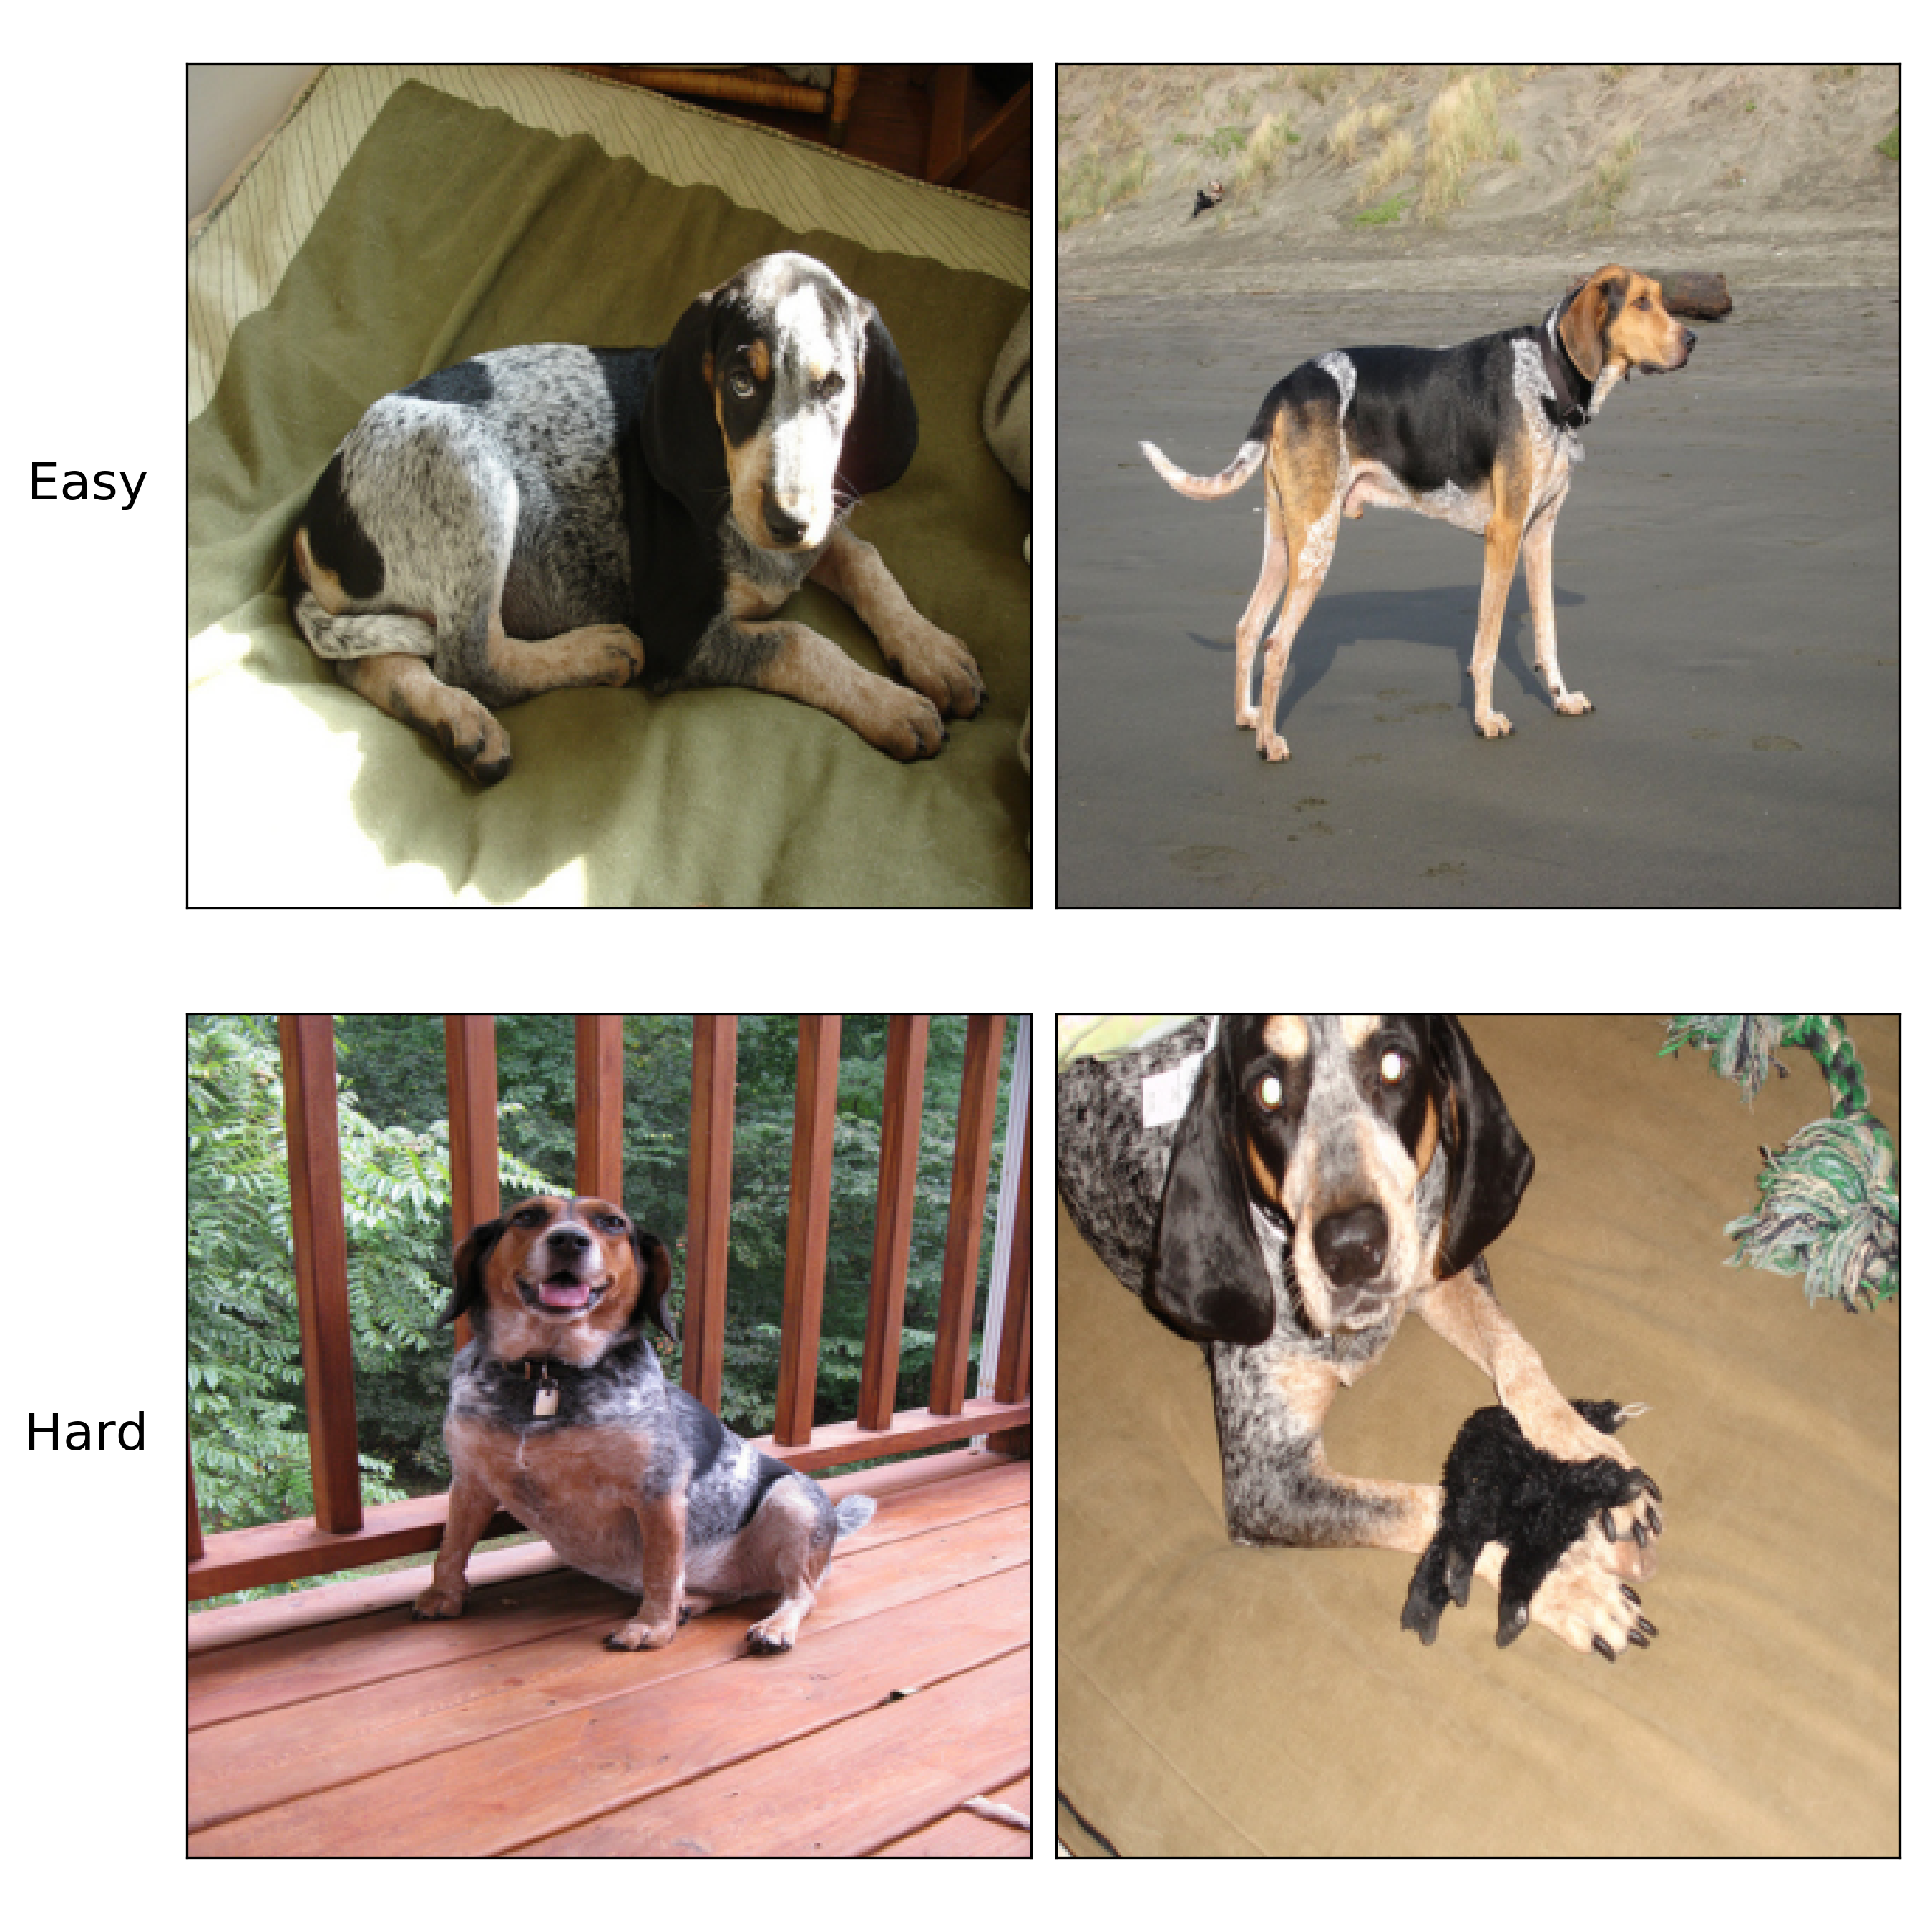
\includegraphics[width=0.45\linewidth]{figures/illustrations/hard_vs_easy_dog}}
	\hfill
	\subfloat[flamingo\label{fig:easyvshardflamingo}]{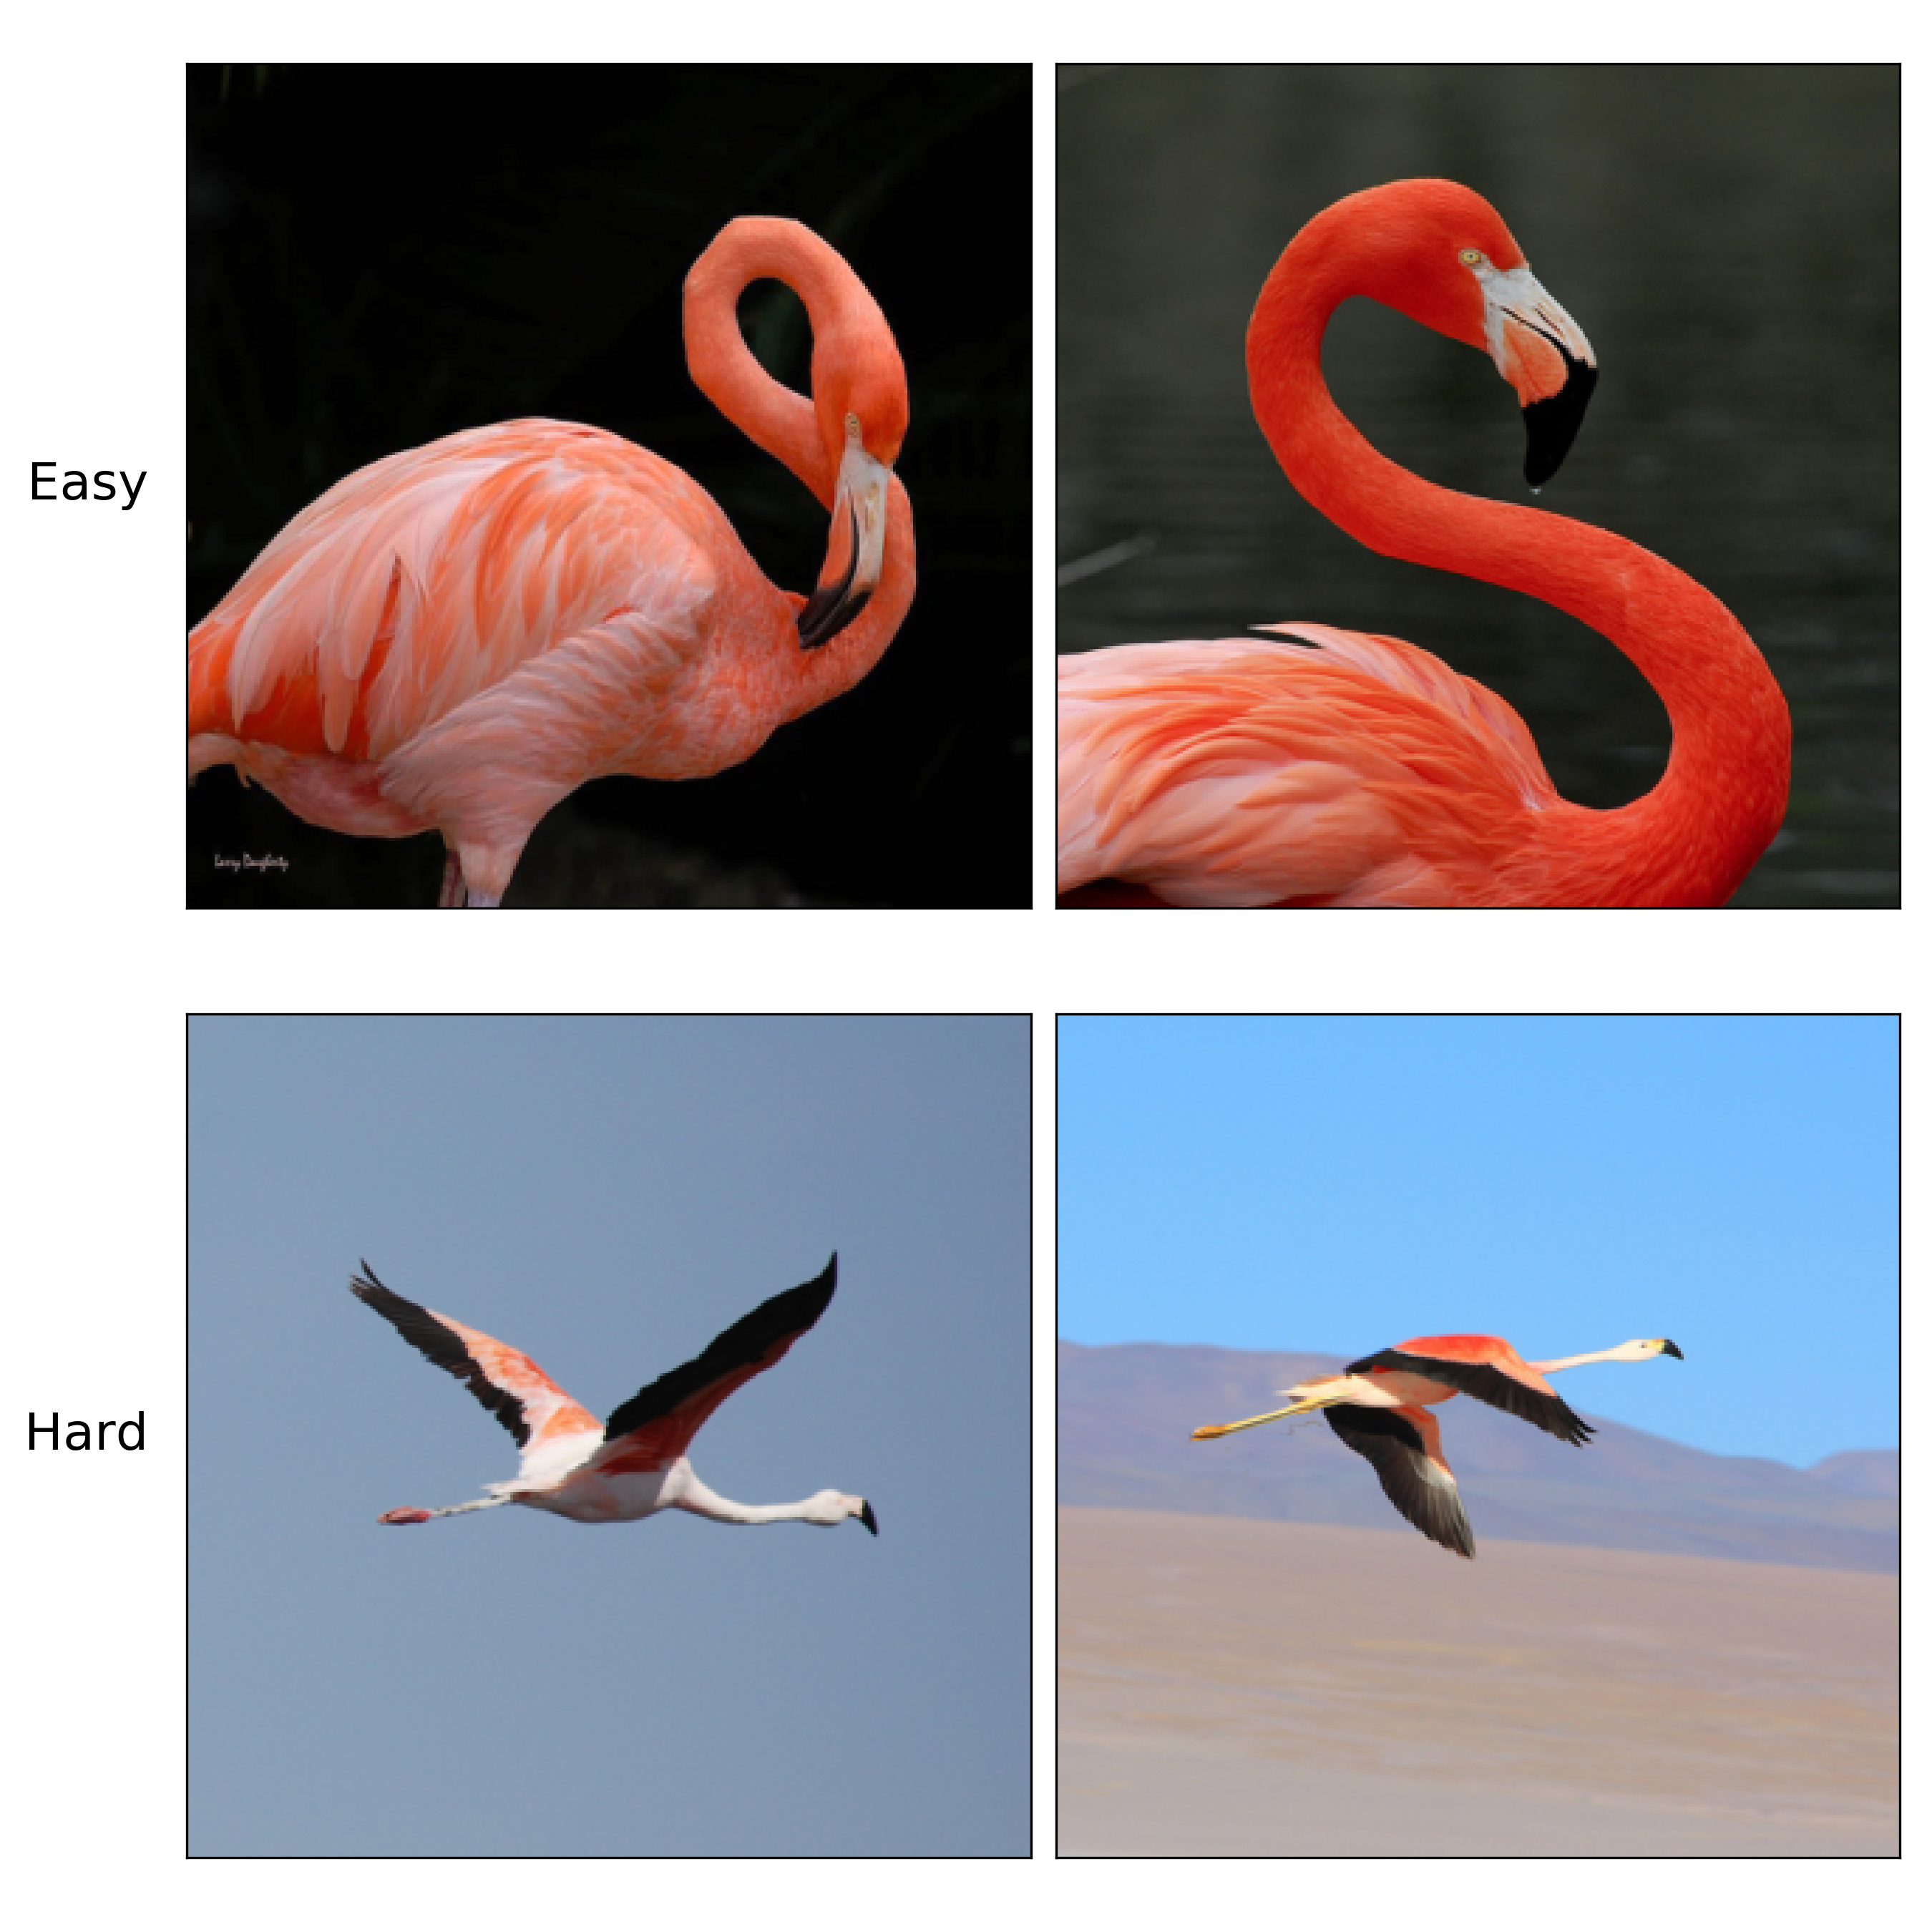
\includegraphics[width=0.45\linewidth]{figures/illustrations/hard_vs_easy_flamingo}}
	\caption[Easy vs. hard samples]{Easy vs. hard samples: The top rows show samples easily classified, and the bottom rows show samples that are more difficult to classify. }
	\label{fig:hardvseasy}
\end{figure}

Figure \ref{fig:hardvseasy} exemplifies samples, where the object is easily separated from the background and is not occluded, are more easily classified. These samples have been found by running an early exit model. The samples are regarded as difficult if the \gls{dnn}s failed to classify or could only correctly classify using the last exit. Samples regarded as easy have been identified by finding samples that could be correctly classified with high confidence by the first exit.

\section{BranchyNet vs. Cascaded DNN} \label{sec:ee-branchy-vs-cascaded}

Both \gls{branchynet} \cite{teerapittayanon_branchynet:_2016} and cascaded \gls{dnn} \cite{leroux_resource-constrained_2015} were published around the same time (\citeyear{teerapittayanon_branchynet:_2016,leroux_resource-constrained_2015}). The cascaded \gls{dnn} adds intermediate classifiers after a layer, or a block of layers in a \gls{dnn}, whereas \gls{branchynet} constructs early exit branches with additional convolution layers, see figure \ref{fig:cascaded-vs-branchy}.

\begin{figure}
	\centering
	\subfloat[Branchy AlexNet, Source \citetitle{teerapittayanon_branchynet:_2016} \cite{teerapittayanon_branchynet:_2016}\label{fig:cascaded-vs-branchy-branchy}]{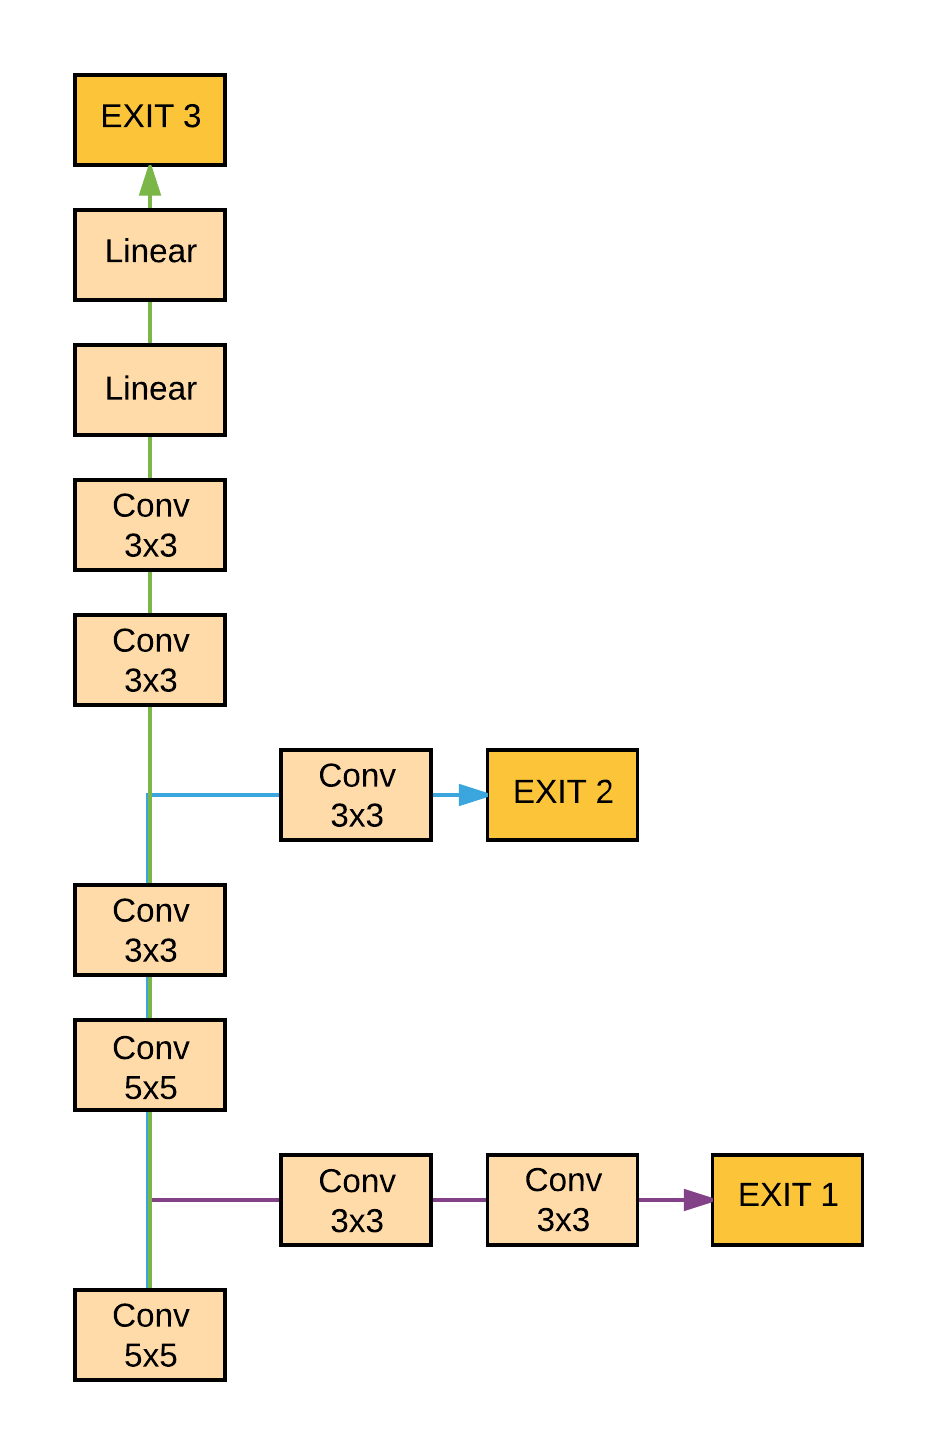
\includegraphics[height=.3\textheight]{figures/articles/branchynet}}
	\hspace{2em}
	\subfloat[Cascaded \gls{dnn}, Source \citetitle{leroux_resource-constrained_2015}\cite{leroux_resource-constrained_2015}\label{fig:cascaded-vs-branchy-cascaded}]{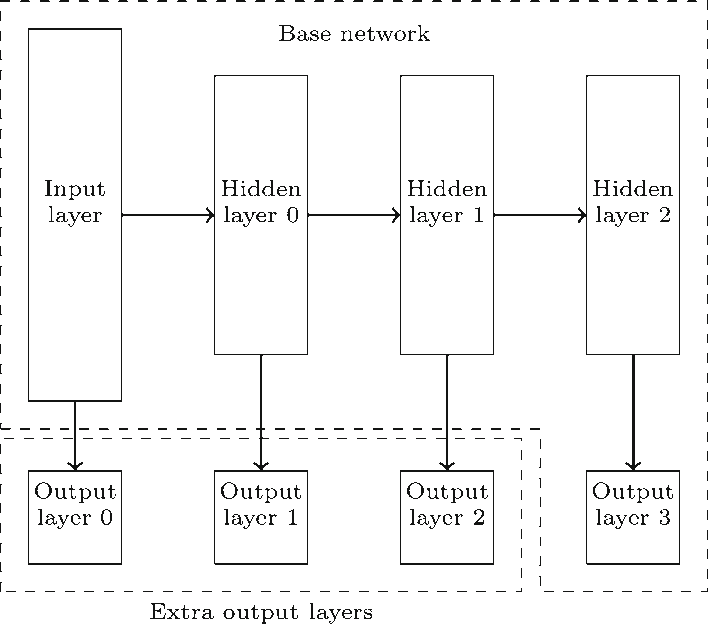
\includegraphics[height=.3\textheight]{figures/articles/cascade_dnn}}
	\caption[\gls{branchynet} vs. Cascaded \gls{dnn}]{\gls{branchynet} vs. Cascaded \gls{dnn}: \protect\subref{fig:cascaded-vs-branchy-branchy} \gls{branchynet} has additional convolution layers in each exit branch, whereas \protect\subref{fig:cascaded-vs-branchy-cascaded} Cascaded \gls{dnn} adds output layers to the layers of the \gls{dnn}.}
	\label{fig:cascaded-vs-branchy}
\end{figure}

Early exiting has shown promising results in other works, e.g., \cite{kaya_shallow-deep_nodate, berestizshevsky_sacrificing_2019,panda_conditional_2016}. In \cite{berestizshevsky_sacrificing_2019}, they suggest removing convolutional layers of branches in \gls{branchynet} to reduce the amount of branch computation. They show a 2 $ \times $ speed-up at only the cost of 1 \% accuracy using two fully-connected layers in exits.
In \cite{kaya_shallow-deep_nodate},  a phenomenon named \emph{overthinking} is studied. Overthinking is an early exit correctly classifying an input, which a later exit would classify incorrectly. In \cite{kaya_shallow-deep_nodate}, they propose to use information from all exits and select the highest scoring prediction to cope with overthinking. We observe the same phenomena for our proposed inference scheme, \gls{aee}, in chapter \ref{ch:edgeoffloading}.

\subsection{Fast Inference Framework} 

The inference framework for the two proposals \gls{branchynet} and Cascaded \gls{dnn}, are almost identical. Samples are inferred to the model, and when reaching an exit, it is decided to terminate or to continue to the next exit based on an exit criterion. 

The algorithm for fast inference using early exit is shown in listing \ref{lst:inference}. 

\begin{minipage}{\linewidth}
	\begin{lstlisting}[language = {}, mathescape=true, caption={Early Exit Fast Inference }, label={lst:inference}]
	procedure $\textsc{EarlyExitFastInference}(i, \gamma)$
	for $n = 1\dots N$ do
	$\bm{z} = f_{exit_n}(i)$
	$ \bm{\hat{y}} = softmax(z) $
	if $\max \bm{\hat{y}} > \gamma$ then
	return $\arg \max \bm{\hat{y}}$
	return $\arg \max \bm{\hat{y}}$ 
	\end{lstlisting}
\end{minipage}

Where $ i $ is the input image, $ \bm{z} $ is the output vector from the last linear layer of an exit, and $ \bm{\hat{y}} $ is the output vector from the softmax function. $ N $ is the number of exits, and $ \gamma $ is the threshold. The softmax function is defined as
\begin{align}
\bm{\hat{y}} = \frac{e^{z}}{\sum_{j=1}^{C}e^{z_c}}
\end{align}

The only inference frameworks are the choice of exit criteria. Cascaded \gls{dnn} uses the softmax score of the prediction. If the score is is higher than a selected threshold, the inference is exited. \gls{branchynet} determines the entropy $ e $ defined by
\begin{align}
e = -\sum_{j=1}^{C} y_c \log \hat{y}_c
\end{align}
and evaluates if the entropy is less than a selected threshold. Note listing \ref{lst:inference} uses the softmax output to evaluate against the threshold.

\subsection{Training Framework} 

In \cite{leroux_resource-constrained_2015}, when training cascaded \gls{dnn}, it is proposed to train a network using a single end-classifier. Once the model has converged, the intermediate classifiers are attached. The entire network is then further trained for one single epoch before freezing the network weights and training only the classifiers, which is equivalent to use a pre-trained model and convert it to a cascaded model. The approach was tested and gave unsatisfactory results, see figure \ref{fig:frozen-b-resnet-miniimagenet-100}. In \cite{leroux_cascading_2017}, they train a frozen base network on the ImageNet dataset but do not achieve better performance than we do when using the same approach.  

The \gls{branchynet} approach is remarkably similar. In \cite{teerapittayanon_branchynet:_2016}, they define the \gls{branchynet} loss function as an extension of the widely used softmax cross-entropy loss function.
\begin{align}
L\left(\bm{y},\hat{\bm{y}}\right) = - \frac{1}{C} \sum_{j =1}^{C} y_c \log \hat{y}_c
\end{align}
Where $ \bm{y} $ is a one-hot encoded ground truth vector, $ \bm{\hat{y}} $ is the output score vector of the softmax classifier and $ C $ is the number of classes and $ c \in \left\{1, 2,  \dots, C\right\} $ is the class labels.
The \gls{branchynet} loss function is defined as the weighted sum of the softmax cross-entropy loss of each branch-prediction. 
\begin{align}
L_{\mathrm{BranchyNet}}(\hat{\bm{y}},\bm{y};\theta) = \sum_{n=1}^{N} w_n L \left(\hat{\bm{y}}_{n},\bm{y};\theta\right)
\end{align}
Where $ \bm{\hat{y}}_n $ is the output score vector of exit $ n $, $ w_n $ is the weight for exit $ n $, and $ \theta $ represents the parameters of the layers from an entry point to the exit point $ n $.

In \cite{teerapittayanon_branchynet:_2016}, they claim that the joint-optimization of multiple exits provide a regularization effect, which improves test accuracy. Additionally, it also mitigates the vanishing gradient problem due to additional gradient signals from the early exits.  In \gls{googlenet} \cite{szegedy_going_2015}, auxiliary classifiers are likewise placed in the middle of the network to counter vanishing gradients. That is also the only purpose of the auxiliary classifiers, as they are only used when training the network. Thus, no samples can exit the inference process. 

In \gls{branchynet}, they have found that higher accuracy can be obtained, and training time can be reduced using a pre-trained conventional \gls{dnn}, and then attach the intermediate classifiers. They do not suggest freezing the model base. To promote more discriminative features in early layers, they train the entire model. We have tried both freezing and unfreezing the network base and have found that training the entire model is by far the most superior approach, which is proved in section \ref{sec:ee-results-training}.

\section{Multi-Scale Dense Network} \label{sec:ee-msdnet}

\gls{msdnet} \cite{huang_densely_2016} addresses two main problems concerning early exit models. The first problem is the lack of coarse-level features in early classifiers, which results in unsatisfactory high error-rates for early exits. Traditional \gls{dnn}s stack layers of convolutions to obtain coarse level features, which the classifiers in shallow layers lack. Multi-scale feature maps preserve high-resolution information and allow the model to construct coarse-level features for all classifiers in the network. 

The second problem is that early classifiers interfere with later classifiers. The early classifiers might cause early features to be optimized for the short-term by collapsing information prematurely, thus harming the later and final classifiers. The \gls{msdnet} \cite{huang_multi-scale_2017} study reveals that densely connected layers suffer less from intermediate classifiers than residual layers. The densely connected layer is connected to all previous layers and is, which enables it to recover collapsed information. The residual and densely connected layers are elaborated upon in section \ref{sec:ee-implementation}.

The combination of multi-scale feature maps for coarse-level features and information preservation from densely connected layers are shown to be important for early exit models. Figure \ref{fig:msdnet} from \cite{huang_multi-scale_2017} shows the model design. On the vertical axis, it shows multi-scale paths that downscale the input images. On the horizontal axis, it shows the stacked densely connected layers. Notice that the concatenation of features (circled c) is done using features from higher scales and from earlier in the same scale-path. Also, note that each block of the \gls{msdnet} contains a classifier.
\begin{figure}
	\centering
	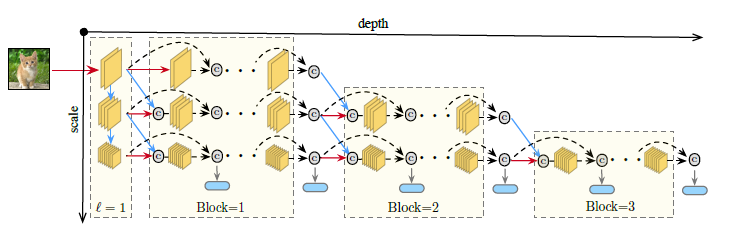
\includegraphics[width=\linewidth]{figures/models/msdnet}
	\caption[\gls{msdnet} Architecture]{\gls{msdnet} Architecture, Source: \citetitle{huang_multi-scale_2017} \cite{huang_multi-scale_2017}}
	\label{fig:msdnet}
\end{figure}

\newpage\section{Analytical Model} \label{sec:ee-metrics}

In this section, we define the analytical model used for our experiments. We compare the conventional models with the early exiting models. Most \gls{dnn}s are built of blocks of convolution and pooling layers. We adapt the same notation for the early exiting inference model and the conventional inference model with a single exit at the end of the \gls{dnn}, see figure \ref{fig:inference_models}.
\begin{figure}
	\centering
	\captionsetup[subfigure]{justification=centering, farskip=1pt,captionskip=1pt}
	\subfloat[Conventional Inference Model]{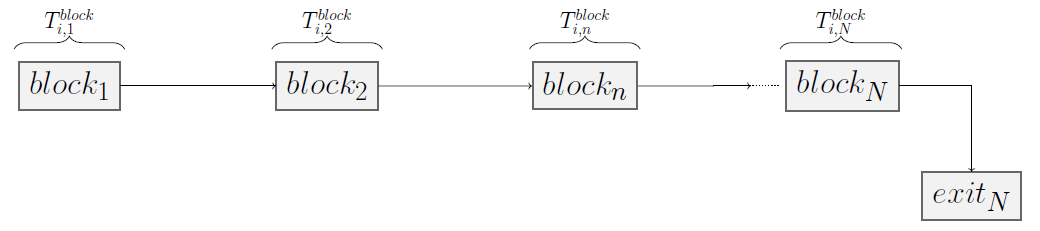
\includegraphics[width=.7\linewidth]{figures/models/conv_math}}
	\hfill
	\subfloat[Early Exit Inference Model]{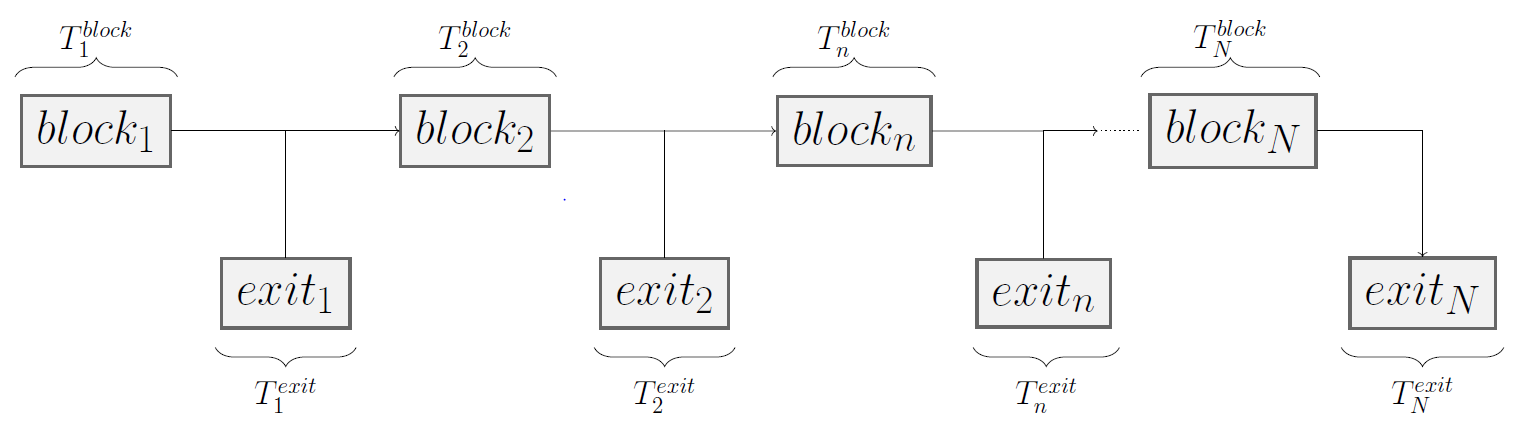
\includegraphics[width=.7\linewidth]{figures/models/exit_math}}
	\caption[\gls{dnn} structure]{\gls{dnn} inference models: A \gls{dnn} is constructed by stacking layers of non-linear function on top of each other to form a \gls{dag}. The layers are typically grouped into blocks, and a classification layer is attached at the end of the network.}
	\label{fig:inference_models}
\end{figure}	
We define the inference latency for both models. We also define classification accuracy, early exit condition and the problem as defined in 5). 

Assume $ C $ denotes the number of image classes, $ N $ denotes the number of the exit points in a DNN, and $ I $ denotes the number of images.

\begin{enumdescript}
	\item[Inference Latency] is defined as the response time for a \gls{dnn} to provide a prediction, i.e., the time from input to output. 
	
	Assume:
	\begin{itemize}
		\item $T_{i,n}^{block}$ denotes the runtime of inferring the image $ i $ in the $ n $th block of the \gls{dnn} for $ \left(1\leq n \leq N, 1 \leq i \leq I\right) $
		\item $T_{i,n}^{exit}$ denotes the runtime of the exit $ n $  to process the image $i$ for $ \left(1\leq n \leq N, 1 \leq i \leq I\right) $
	\end{itemize}
	\begin{enumdescript}
		\item[Inference Latency in Conventional Model] The conventional inference model has a single exit at block $ N $, hence all $ N $ blocks of the \gls{dnn} must have processed the image $ i $ before a classification is reached at exit $ N $. Thus the runtime to classify the image $ i $ using a conventional model is described as
		\begin{align}
		T^{ci}_{i}= \sum_{j=1}^{N} T_{i,n}^{block} + T_{i,N}^{exit}
		\end{align}
		\item[Inference Latency in Early Exit Model] The early exit inference model is adaptive. The inference of the image $ i $ can terminate at any exit $ n $. If the classification exits from exit point $ n $, then the latency model for early exit inference model is presented as
		\begin{align}
		T_{i,n}^{ee}=\sum_{j=1}^{n} \left(T_{i,n}^{block} + T_{i,n}^{exit} \right) 
		\end{align}
		The additional classifiers of the early exit inference model add a small delay overhead compared to the conventional inference model. However, it may not be required to run all $ n $ blocks and classifiers of the early exit inference model. 
	\end{enumdescript}
	
	\item[Classification Accuracy] is the defined as the fraction of correctly classified samples out of all inferred samples. The inference accuracy can be expressed as
	\begin{align}
	\bar{A}=1-\frac{1}{I} \sum_{i=1}^{I} \mathbb{I}\left(\left|\hat{c}_{i}-c_{i}\right|\right) \label{eq:accuracy}
	\end{align}
	%We can express the ground truth as a one-hot encoded vector $ \bm{y}_i $
	where $ \mathbb{I(\cdot)}  $ is an indicating function defined by
	\begin{align}
	\mathbb{I}(a)= \begin{cases}
	0, & \mathrm{if\:} a \leq 0, \\
	1, & \mathrm{otherwise}
	\end{cases} \label{eq:indicator}
	\end{align}
	and $ c_i \in \left\{1, 2, \dots, C \right\} $ is the ground truth class label of the image $ i $, and $  \hat{c}_i \in \{\hat{c}^*_{i,1} , \hat{c}^*_{i,2}, \dots, \hat{c}^*_{i,N} \} $ is the predicted class for the image $ i $. 
	
	It means the prediction of any exit point can be used as the output of DNN. Each element $ \hat{c}^*_{i,n} $ in the set denotes the predicted class of exit point $ n $, which is the class with the maximum confident score, i.e.,
	\begin{align}
	\hat{c}^*_{i,n} = \arg \underset{c}{\max}\: \bm{\hat{y}}_{i,n}
	\end{align}
	where $ \bm{\hat{y}}_{1,n} $ is the confidence score vector output from the softmax classifier of exit point $ n $, i.e.,
	\begin{align}
	\bm{\hat{y}}_{i,n} = \left[\begin{array}{ccccc}\hat{y}_{i,n,1} & \hat{y}_{i,n,2} & \hat{y}_{i,n,c} & \dots & \hat{y}_{i,n,C}\end{array}\right]
	\end{align}
	Each element $ \hat{y}_{i,n,c} \in \bm{\hat{y}}_{i,n} $ represents the score of class $ c $ from exit point $ n $ by processing the image $ i $.
	
	Note the accuracy for each exit can be expressed as
	\begin{align}
	\bar{A}_n=1-\frac{1}{I} \sum_{i=1}^{I} \mathbb{I}\left(\left|\hat{c}^*_{i,n}-c_{i}\right|\right)
	\end{align}
	
	\item[Early Exit Condition] we define the early exit condition based on the output of our scoring function $ f_\phi(\bm{\hat{y}}_{i,n}) $. The function takes the score vector $ \bm{\hat{y}}_{i,n} $ for the image $ i $ at exit point $ n $ as input. The image $ i $ is allowed to exit the model at exit point $ n $ if a score threshold $ \gamma $ is surpassed. 
	
	All scores of  $ \bm{\hat{y}}_{i,n} $ sum to 1 hence we assume $	\gamma \in \left[0,1\right] $. Note that although the score threshold could be different for each exit point since we are concerned with latency, we use the same threshold in our experiments. Selecting a high threshold value at an early exit will cause fewer samples to exit and promote the use of later exits, which will cause additional inference delay. It is seen in \cite{teerapittayanon_finding_2018}, that finding different threshold values for the exits can improve the accuracy.
	
	We express the probability of early exit at exit $ n $		\begin{align}
	\overline{F}^{exit}_n = \frac{1}{I}\sum_{i=1}^{I} \mathbb{I} \left(\gamma-f_{\phi}\left(\bm{\hat{y}}_{i,n}\right) \right)
	\end{align}
	where $ f_\phi\left(\bm{\hat{y}}_{i,n}\right) $ is a scoring function, and for notation simplicity, we write 
	\begin{align}
	f_{\phi}\left(\bm{\hat{y}}_{i,n}\right) = \begin{cases}
	f_{max}\left(\bm{\hat{y}}_{i,n}\right)\\
	f_{margin}\left(\bm{\hat{y}}_{i,n}\right)
	\end{cases}
	\end{align}
	which means we can choose to use either one. Next, we define two different score functions.
	
	\begin{enumdescript}
		\item[Score-Max] the score-max function $ f_{max}(\cdot)$ also used in \cite{leroux_resource-constrained_2015}, takes the score vector $ \bm{\hat{y}}_{i,n} $ of the image $ i $ at exit $ n $ as input and outputs the maximum value of the vector. It is expressed as
		\begin{align}
		f_{max}\left(\bm{\hat{y}}_{i,n}\right) = \underset{c}{\max} \bm{\hat{y}}_{i,n}
		\end{align}
		\item[Score-Margin] the score-margin function $ f_{margin}(\cdot)$, is defined and used in \cite{park_big/little_2015}. The function also takes the score vector $ \bm{\hat{y}}_{i,n} $ as input and returns the difference between the two largest elements. It is expressed as
		\begin{align}
		f_{margin}\left(\bm{\hat{y}}_{i,n}\right) = \hat{y}_{i,n}^{1st} - \hat{y}_{i,n}^{2nd} \label{eq:f_margin}
		\end{align}
		where $ \hat{y}_{i,k}^{1st} $ denotes the largest element and $ \hat{y}_{i,n}^{2nd} $ the second largest element of $ \bm{\hat{y}}_{i,n} $.
		
	\end{enumdescript}
	
	\item[Reliability] Our primary concern is time-critical application; hence we define the reliability as the obtainable accuracy before a deadline $ \delta $. 	
	\begin{align}
	R= \bar{A} \cdot (1-\overline{F}^{to})
	\end{align}
	
	We formulate the timeout probability $ \overline{F}^{to} $ as the number of samples not able to meet the deadline out of all samples in the set.
	\begin{align}
	\overline{F}^{to}=\frac{1}{I}\sum_{i=1}^{I} \mathbb{I}\left(T_{i}^{cmp}-\delta\right)
	\end{align}
	Where $ T_{i}^{cmp} $ denotes the runtime to process the image $i$. We can choose between a conventional model or an early exit model 
	\begin{align}
	T^{cmp}_i = \begin{cases}
	T^{ci}_i \\
	T^{ee}_i
	\end{cases} \label{eq:t_ci-and-t_ee}
	\end{align}
	We only have a delay violation if $ T_i^{cmp} \leq \delta $, i.e., the model has not provided prediction from any exit within the time frame. Thus, if no exit of the model can meet the delay requirements for the image $i$ it is treated as a misclassification. 
	
	\item[Problem formulation] We aim to maximize the reliability for each image by selecting the best possible exit
	\begin{maxi}
		{\bm{n}}{R}
		{}{}
	\end{maxi}
	where $ \bm{n} = \left[ n_1, n_2, \dots, n_I \right]$ is a vector to denote which exit point would be used for prediction of the image $ i $ for available exit point $ n_i \in \left\{1,2, \dots, N\right\} $.
	
	To solve this problem, instead of deciding exit for the image, we use the best effort, i.e., feed each exit results back and let the user decide the prediction. For three reasons:
	\begin{enumerate}
		\item latency uncertainty makes it hard to decide in advance
		\item algorithm to make the decision may take time
		\item going through the classifier of each exit point would not take a too long time.
	\end{enumerate}
	
\end{enumdescript}

\section{Implementation} \label{sec:ee-implementation}

In this section, we describe our implementation of early exit models. We have implemented \gls{bresnet} and \gls{bdensenet} based on existing \gls{resnet}101 and \gls{densenet}-121 respectively. We reused those architectures to avoid training models from scratch due to the project's time constraint. Reusing enabled us to initialize the models with publicly available weights trained on the entire ImageNet dataset.

\subsection{Branchy-ResNet} 

Residual Networks or \gls{resnet}s \cite{he_deep_2015} have, for long, been state-of-the-art and won ILSVRC15 using 152 layers. The residual layers are the building blocks of the residual networks. The residual layers have made it possible to train extremely deep networks. The depth of \gls{dnn}s is of paramount importance to extract increasingly richer features from images to obtain highly accurate classification models. Training plain \gls{vgg} networks \cite{simonyan_very_2015} with more than ten layers to convergence is not easy due to vanishing/exploding gradients. To mitigate this problem, the \gls{resnet} adds a shortcut connection, which skips a layer or a block of layers. Information from earlier layers is preserved by the skip connection, which diminishes the vanishing gradient problem. Thus, this type of network has proved to be easier to train compared to plain networks and obtains far superior accuracy. The skip connection adds the identity of the input to the output of the layer or block, see figure \ref{fig:residualblock}

\begin{figure}
	\centering
	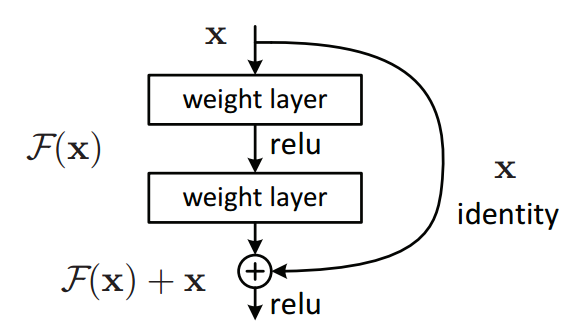
\includegraphics[width=.5\linewidth]{figures/models/residualblock}
	\caption[Residual Block]{Residual Block: A residual block adds the identity, i.e., the input to the layer or block of layers to the output of the block. Source: \citetitle{he_deep_2015} \cite{he_deep_2015}}
	\label{fig:residualblock}
\end{figure}

The residual networks proposed in \cite{he_deep_2015} are grouped into four resolution blocks, each of which downsamples the input data. The networks are designed with a different number of layers $ \left\{18, 34, 50, 101, 152\right\} $, exemplifying the ability to train extremely deep networks. Table \ref{tbl:resnet101} describes the blocks and layers of the \gls{resnet}101 architecture. \gls{pytorch} provides implementations in different types of networks. These models can be trained from scratch or initialized with downloadable pre-trained weights based on ImageNet. The weight is available trough a \gls{pytorch} API. \gls{resnet}101 has been chosen for this project as it has comparable depth to the smallest available \gls{pytorch} \gls{densenet}-121 implementation and also have similar inference latency on a Titan Xp (8.90ms vs. 8.93ms) \cite{bianco_benchmark_2018}.

\small
\begin{center}
	
	\begin{minipage}[c]{\linewidth}
		\begin{longtabu}{>{\bfseries}X|X[c]|X[2c]}
			\caption[\gls{resnet}101 description]{The table describes the blocks of \gls{resnet}101, the size of the block, and the layers of the block. Note, a pooling layer is placed at the end of each resolution block to downsample the data size.} \label{tbl:resnet101} \\
			\toprule
			\rowfont{\bfseries}
			Resolution block & Output size & Layer description \tabularnewline
			\hline
			\endfirsthead
			\multicolumn{3}{@{}l}{\textbf{\textcolor{black}{Table \ref{tbl:resnet50}:}} continued}\\
			\toprule
			\rowfont{\bfseries}
			Conv block & Output size & Layer description \tabularnewline
			\hline
			\endhead % all the lines above this will be repeated on every page
			\hline
			\multicolumn{3}{@{}l}{continued \ldots}\\
			\endfoot
			\hline
			\endlastfoot
			conv1 & $112\times 112$& $7\times 7, 64, \:\mathrm{stride}\: 2$ \tabularnewline \hline
			
			\multirow{5}{*}{conv2\_x} 	& \multirow{5}{*}{$56 \times 56$} 	& $3 \times 3 \:\mathrm{maxpool, stride}\: 2 $ \\ \tabucline{3-3} & & \multirow{4}{*}{
				$\begin{bmatrix}
				1 \times 1, 64 \\ 3 \times 3, 64 \\1 \times 1, 256
				\end{bmatrix} \times 3$ }		\tabularnewline										
			& & 	\tabularnewline
			& & 	\tabularnewline
			& & 	\tabularnewline
			\hline
			
			\multirow{4}{*}{conv3\_x} 	& \multirow{4}{*}{$28\times 28$} & \multirow{4}{*}{
				$\begin{bmatrix}
				1 \times 1, 128 \\ 3 \times 3, 128 \\1 \times 1, 512
				\end{bmatrix} \times 4$ }		\tabularnewline										
			& & 	\tabularnewline
			& & 	\tabularnewline
			& & 	\tabularnewline
			\hline
			
			\multirow{4}{*}{conv4\_x} 	& \multirow{4}{*}{$14\times 14$} & \multirow{4}{*}{
				$\begin{bmatrix}
				1 \times 1, 256 \\ 3 \times 3, 256 \\1 \times 1, 1024
				\end{bmatrix} \times 23$}		\tabularnewline										
			& & 	\tabularnewline
			& & 	\tabularnewline
			& & 	\tabularnewline
			\hline
			
			\multirow{4}{*}{conv5\_x} 	& \multirow{4}{*}{$7\times 7$} & \multirow{4}{*}{
				$\begin{bmatrix}
				1 \times 1, 512 \\ 3 \times 3, 512 \\1 \times 1, 2048
				\end{bmatrix} \times 3$}		\tabularnewline										
			& & 	\tabularnewline
			& & 	\tabularnewline
			& & 	\tabularnewline
			\hline
			
			Classifier & \multicolumn2{c}{$\mathrm{Avg.\: Pool,\:} 1000d\: \mathrm{fc,\: Softmax}$} \tabularnewline
			\bottomrule
		\end{longtabu}
		\color{caption-color}{\textit{Source: \citetitle{he_deep_2015}, by \citeauthor{he_deep_2015} \cite{he_deep_2015}, describes a full list of Residual Networks (\gls{resnet}18, \gls{resnet}34, \gls{resnet}50, \gls{resnet}101, and \gls{resnet}152)}}\color{main-color}
	\end{minipage}
\end{center}
\normalsize
To construct the early exits model, a pooling-layer followed by a fully-connected linear with the softmax classifier is added. Figure \ref{fig:b-resnet} illustrates the early exiting model \gls{bresnet}.
\begin{figure}
	\centering
	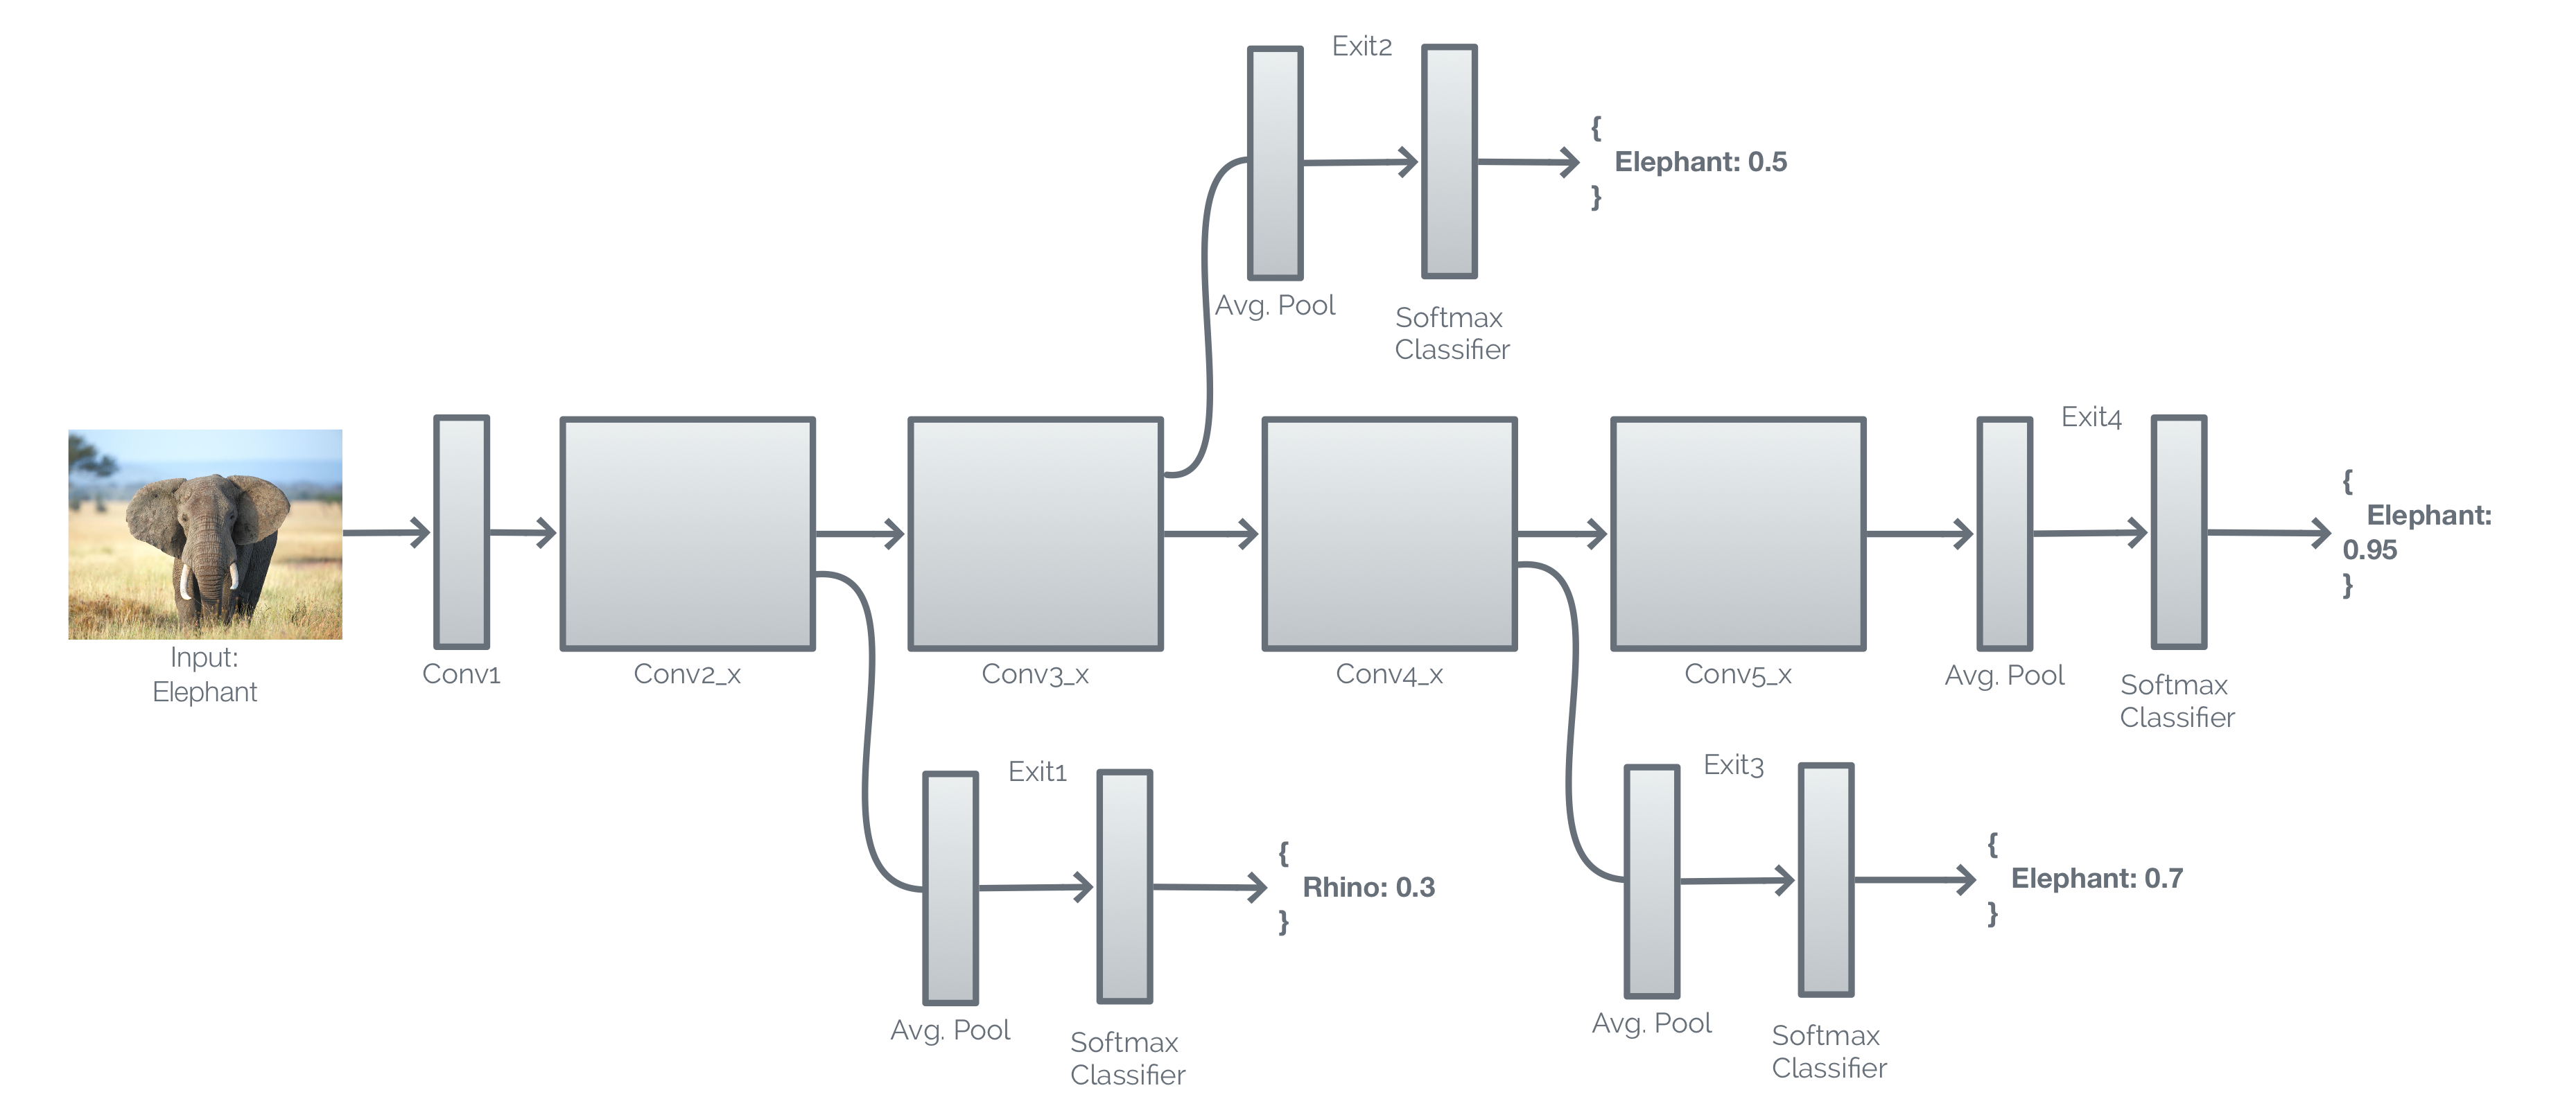
\includegraphics[width=\linewidth]{figures/models/BResNet}
	\caption[B-\gls{resnet} architecture]{\gls{bresnet}: extending the \gls{resnet}101 to implement the BranchyNet framework. The figure illustrates how classification confidence grows as we go deeper in the model. Note, The first exit actually fails to classify the elephant. }
	\label{fig:b-resnet}
\end{figure}
The early exits of \gls{bresnet} are placed immediately after a resolution block, as;
\begin{enumerate}
	\item The exit must be placed sufficiently deep so that the model can predict some input samples correctly
	\item If used in a collaborative setup, a smaller feature representation is desired to reduce the offloaded data size. The exits are placed after the resolution block, as the filter size is unchanged within the block \cite{eshratifar_bottlenet:_2019}. 
\end{enumerate}


\newpage\subsection{Branchy-DenseNet}

Densely Connected Network or \gls{densenet} is proposed in \cite{huang_densely_2016}. In \cite{huang_densely_2016}, it discovered that many of the residual layers in \gls{resnet}s only have a small contribution to the output, and can be dropped during training. \gls{densenet} combines features from all subsequent layers by concatenation, as there is no need to re-learn redundant information by adding previously learned information to the output. Figure \ref{fig:densenet} shows the dense connections that combine features from all subsequent layers in a block. Note, the feature size grows throughout a densely connected block as a result of concatenation. Therefore the \gls{densenet} can be thinner as the number of channels can be fewer, which makes it more efficient compared to plain and residual networks. Additionally, densely connected blocks have a regularizing effect, thus reducing overfitting and have shown to train better on smaller data sets.

\begin{figure}
	\centering
	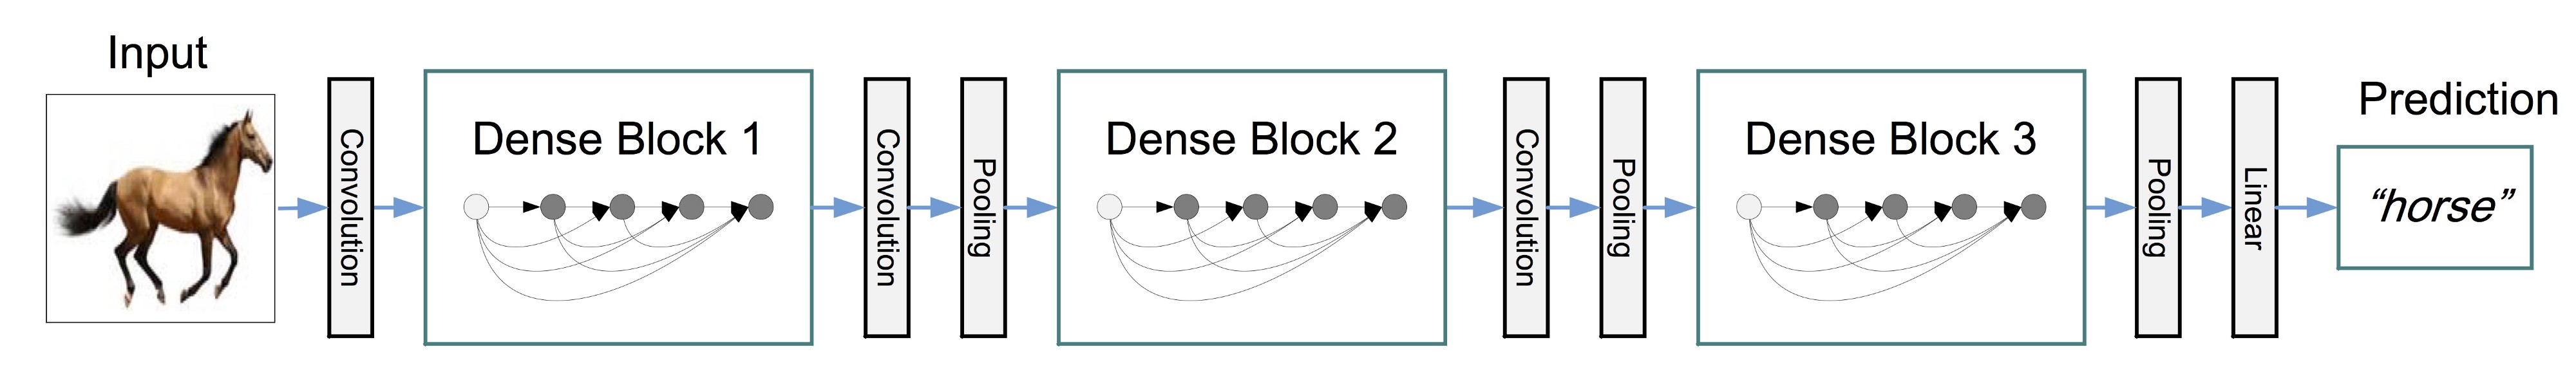
\includegraphics[width=\linewidth]{figures/models/densenet}
	\caption[\gls{densenet}]{\gls{densenet}: The densely connected layers are similarly grouped into blocks called dense blocks. Source: \citetitle{huang_densely_2016} \cite{huang_densely_2016}.}
	\label{fig:densenet}
\end{figure}

Table \ref{tbl:densenet121} describes the block and layers of the \gls{densenet} architecture. 

In \cite{huang_multi-scale_2017}, they argue, that the collective knowledge from all preceding layers of \gls{densenet} gives more diversified features compared to the correlated features of \gls{resnet}s. In \cite{huang_multi-scale_2017}, the diversified features are shown to be more suited for early exiting, as the information is better preserved using densely connected layers. Additionally, they show the placement of an intermediate classifier in a \gls{densenet} has less impact on the learned features for a later classifier. They argue that the collapsed information to generate a short-term feature for an earlier classifier can be restored by the dense connections for a later classifier.
\begin{small}
	\begin{minipage}[c]{\linewidth}
		\begin{longtabu}{>{\bfseries}X|X[c]|X[2c]}
			\caption[\gls{densenet}-121 description]{\gls{densenet}-121 description. The table describes the blocks of \gls{densenet}-121. $k$ is the growth rate of the DenseBlock. A typical setting is $k=32$ yielding 256, 512, and 1024 output channels for denseblock(1-3) respectively. The transition layer downsamples the output channel by a factor of 2, thus the number of input channels for DenseBlock(2-4) becomes 128, 256, and 512 respectively.} \label{tbl:densenet121} \\
			\toprule
			\rowfont{\bfseries}
			Layers & Output size & Layer description \tabularnewline
			\hline
			\endfirsthead
			\multicolumn{3}{@{}l}{\textbf{\textcolor{black}{Table \ref{tbl:resnet50}:}} continued}\\
			\toprule
			\rowfont{\bfseries}
			Layers & Output size & Layer description \tabularnewline
			\hline
			\endhead % all the lines above this will be repeated on every page
			\hline
			\multicolumn{3}{@{}l}{continued \ldots}\\
			\endfoot
			\hline
			\endlastfoot
			Convolution & $112\times 112$& $7\times 7, \:\mathrm{stride}\: 2$ \tabularnewline \hline
			Pooling & $56\times 56$& $3\times 3, \:\mathrm{maxpool},\:  \mathrm{stride}\: 2$ \tabularnewline \hline
			\multirow{3}{*}{DenseBlock (1)} 	& \multirow{3}{*}{$56 \times 56$} & \multirow{3}{*}{
				$\begin{bmatrix}
				1 \times 1, k \\ 3 \times 3, k \\
				\end{bmatrix} \times 6$ }		\tabularnewline										
			& &  	\tabularnewline
			& & 	\tabularnewline
			\hline
			
			Transition  	& $56 \times 56$ & $1 \times 1\: \mathrm{conv}$ \tabularnewline \tabucline{2-3}							
			Layer (1) & $28\times 28$ & $2\times 2\: \mathrm{average\: pool,\: stride}\: 2$	\tabularnewline
			
			\hline
			
			\multirow{3}{*}{DenseBlock (2)} 	& \multirow{3}{*}{$28 \times 28$} & \multirow{3}{*}{
				$\begin{bmatrix}
				1 \times 1, k \\ 3 \times 3, k \\
				\end{bmatrix} \times 12$ }		\tabularnewline										
			& &  	\tabularnewline
			& & 	\tabularnewline
			\hline
			
			Transition  	& $28 \times 28$ & $1 \times 1\: \mathrm{conv}$ \tabularnewline \tabucline{2-3}							
			Layer (2) & $14\times 14$ & $2\times 2\: \mathrm{average\: pool,\: stride}\: 2$	\tabularnewline
			
			\hline
			
			\multirow{3}{*}{DenseBlock (3)} 	& \multirow{3}{*}{$14 \times 14$} & \multirow{3}{*}{
				$\begin{bmatrix}
				1 \times 1, k \\ 3 \times 3, k \\
				\end{bmatrix} \times 24$ }		\tabularnewline										
			& &  	\tabularnewline
			& & 	\tabularnewline
			\hline
			
			Transition  	& $14 \times 14$ & $1 \times 1\: \mathrm{conv}$ \tabularnewline \tabucline{2-3}							
			Layer (3) & $7\times 7$ & $2\times 2\: \mathrm{average\: pool,\: stride}\: 2$	\tabularnewline
			
			\hline
			
			\multirow{3}{*}{DenseBlock (4)} 	& \multirow{3}{*}{$7 \times 7$} & \multirow{3}{*}{
				$\begin{bmatrix}
				1 \times 1, k \\ 3 \times 3, k \\
				\end{bmatrix} \times 16$ }		\tabularnewline										
			& &  	\tabularnewline
			& & 	\tabularnewline
			\hline
			
			Classification  	& $1 \times 1$ & $7 \times 7\: \mathrm{global\: average\: pool}$ \tabularnewline \tabucline{2-3}							
			Layer &  \multicolumn2{c}{$\mathrm{Avg.\: Pool,\:} 1000d\: \mathrm{fc,\: Softmax}$} \tabularnewline
			\bottomrule
		\end{longtabu}
		\color{caption-color}{\textit{Source: \citetitle{huang_densely_2016}, by \citeauthor{huang_densely_2016} \cite{huang_densely_2016}, describes a full list of Densely Connected Networks (\gls{densenet}-121, \gls{densenet}-169, \gls{densenet}-201 and \gls{densenet}-264)}} \color{main-color}
	\end{minipage}
\end{small}
In the same manner, as for \gls{resnet} exits consisting of a pooling layer and a linear classifier is attached to the model.
\begin{figure}
	\centering
	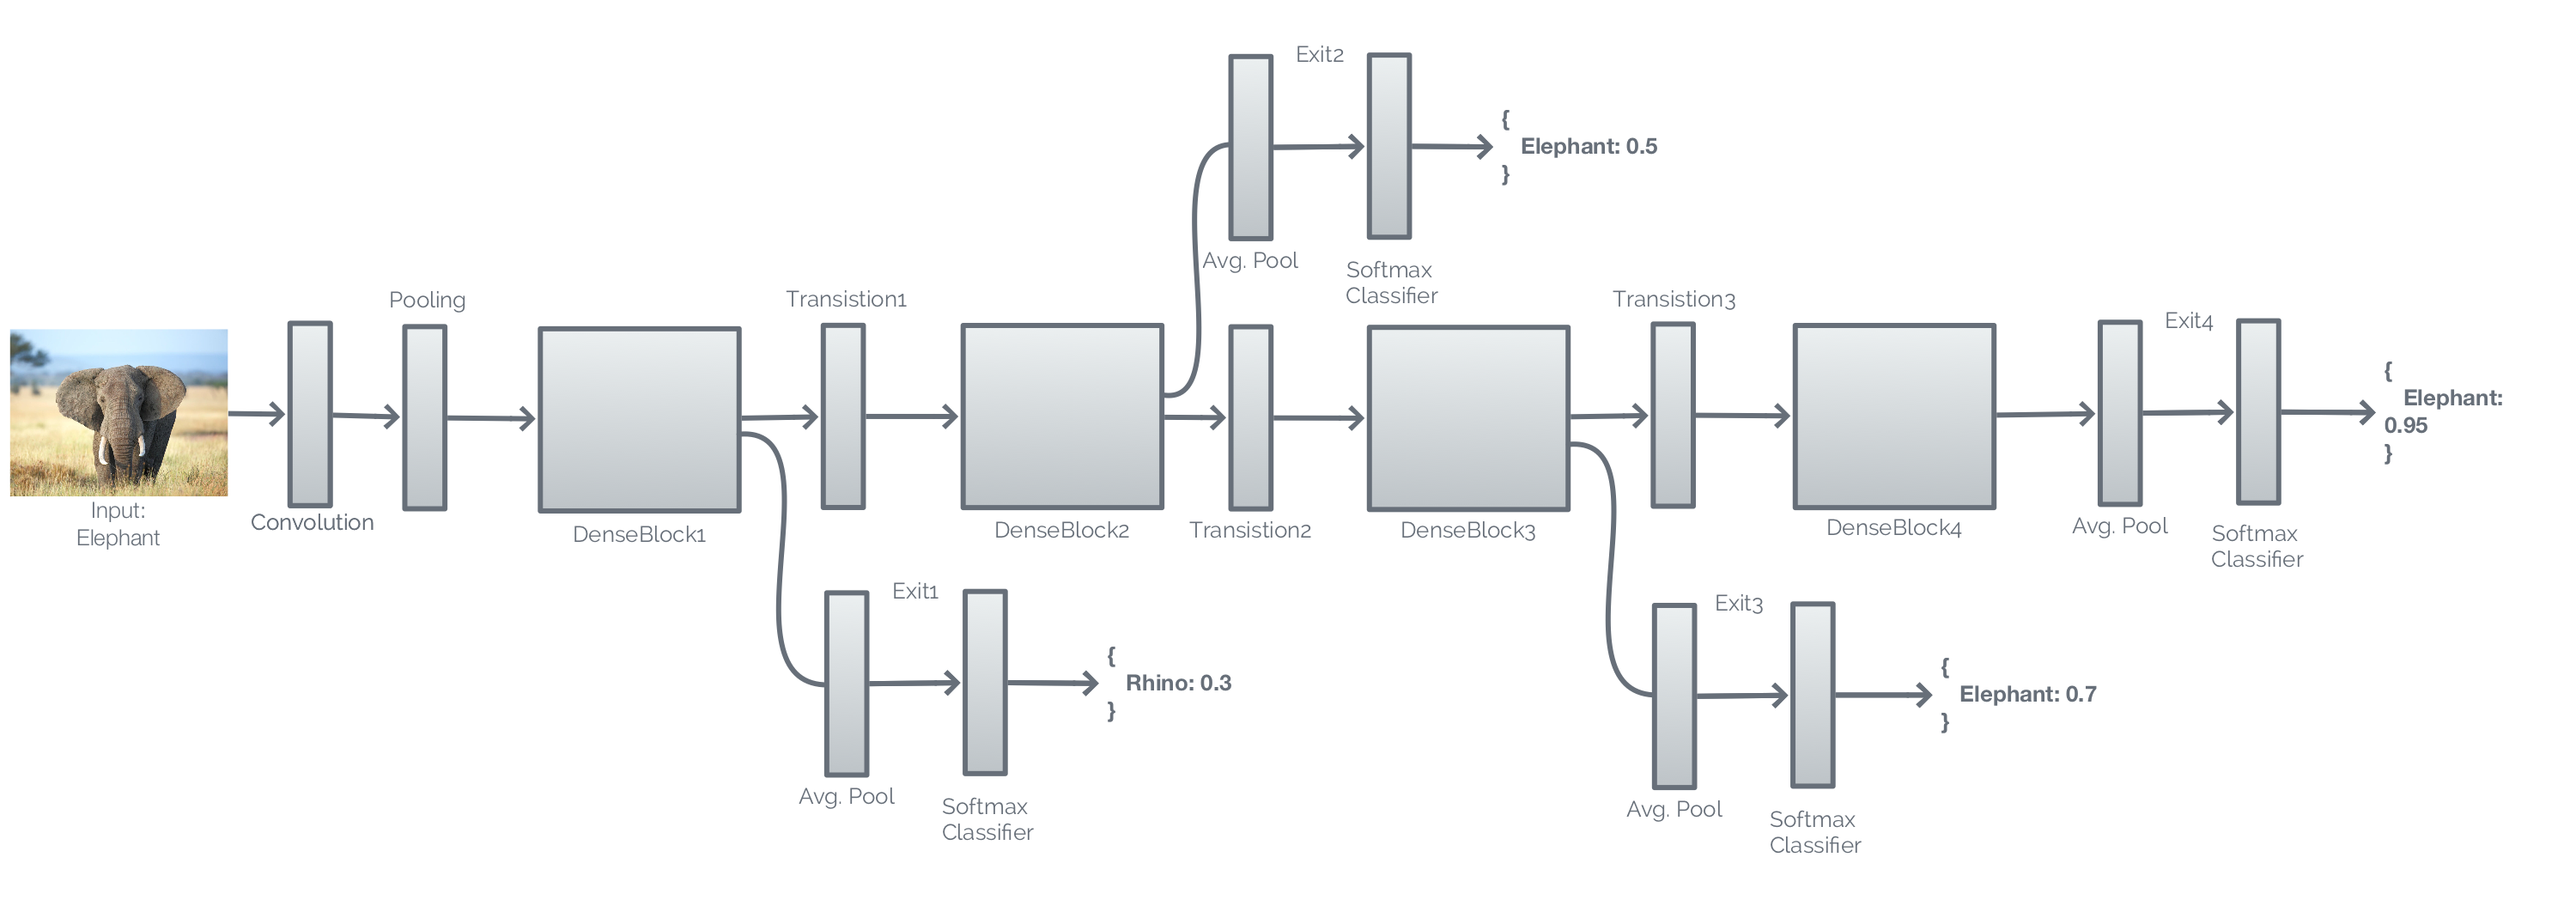
\includegraphics[width=\linewidth]{figures/models/b-densenet}
	\caption[B-\gls{densenet} architecture]{\gls{bdensenet}: \gls{densenet}-121 extended to implement the \gls{branchynet} framework. The figure illustrates the placement of exits after a densely connected block. If the sample could not be exited, the inference continues to the transition layer, which downsamples the input for the next dense block. }
	\label{fig:b-densenet}
\end{figure}
For the \gls{bdensenet}, we place the exits after the densely connected blocks, for two reasons: 
\begin{enumerate}
	\item We must go sufficiently deep to obtain features that can correctly classify some samples.
	\item We place exits before the transition layer to avoid unnecessary downsampling if exiting is already possible. 
\end{enumerate}
Note, partitioning for remote execution is done after the transition layer, as a smaller data size can be offloaded. Figure \ref{fig:b-densenet} illustrates the exit placement.

The early exits were placed after down-sampling layers or block, with the primary reason to reduce the offloading data size of intermediate features for collaborative inference on edge. However, in \cite{huang_multi-scale_2017}, the placement of early exit is placed within the resolution- and dense blocks. They implement new versions of the \gls{resnet} and \gls{densenet} with the same number of layers within each block. They evenly distributed two exits within each block, i.e., eight exits in all. We limited ourselves to only four early exits classifiers, in order not to slow the interference process. In fact, in \cite{berestizshevsky_sacrificing_2019}, the same placement of classifiers is used. To limit the delay overhead and reduce wasted computation if samples cannot be exited. Our exits only consist of a pooling layer to reduce the feature size and a linear classifier, as in \cite{kaya_shallow-deep_nodate}, whereas in \cite{teerapittayanon_branchynet:_2016}, they add convolution layers in exit branches. 


\section{Experimental Setup} \label{sec:ee-exp-setup}

All code is written in \gls{python} 3.7 \cite{van_rossum_python_1995} using the \gls{pytorch} 1.2
framework \cite{paszke_automatic_2017} and using the \gls{torchvision} 0.4 library \cite{marcel_torchvision_2010}. All code is available at
{\color{sns-grey}\url{https://github.com/AlexKarlsen/thesis-src}}. 

Table \ref{tbl:platforms} lists the hardware platforms used for the experiments and their characteristics. Table \ref{tbl:models} lists the models used in the experiment and compares the number of layers, parameters, and \acrshort{flop}s of the models. The number of parameters and \acrshort{flop}s have been found using \gls{thop} \cite{zhu_thop_nodate}, by inference a random 4d tensor of size $ (\mathrm{batch,channels,width,height})=(1,3,224,224) $ to all models. Note, only a small overhead in the number of parameters and \acrshort{flop}s is added for the early exit models compared to the conventional models. Thus, we expect only a small additional delay from the intermediate classifiers, which is proved in section \ref{sec:edge-results}.

\begin{minipage}[t]{\linewidth}
	\begin{longtabu}{>{\bfseries}X[0.8]|X[0.8]|X[1.5]|X[r0.3]}
		\caption[Platform hardware comparison]{Platform hardware comparison of Window 10 Stationary PC named \gls{gpu-ws}, an NVIDIA \gls{jetson} development edge computer, and an Intel \gls{nuc} mini pc} \label{tbl:platforms} \\
		\toprule
		\rowfont{\bfseries}
		Platform & CPU & GPU & RAM  \tabularnewline
		\bottomrule
		\endfirsthead
		\multicolumn{3}{@{}l}{\textbf{\textcolor{black}{Table \ref{tbl:platforms}:}} continued}\\
		\toprule
		\rowfont{\bfseries}
		Platform & CPU & GPU & RAM  \tabularnewline
		\bottomrule
		\endhead % all the lines above this will be repeated on every page
		\bottomrule
		\multicolumn{3}{@{}l}{continued \ldots}\\
		\endfoot
		\hline
		\endlastfoot
		GPU Workstation	& Intel i5-6600K.	& NVIDIA GeForce GTX 1080, 2560 CUDA cores	& 16GB \tabularnewline
		\hline
		Jetson TX2	& ARM Cortex-A57 	& NVIDIA Pascal GPU, 256 CUDA cores 		& 8GB \tabularnewline
		\hline
		NUC		  	& Intel i7-7567U	& None										& 16GB \tabularnewline									
		\bottomrule
	\end{longtabu}
\end{minipage}
%equipped with a NVIDIA GeForce 1080 GTX \gls{gpu} using CUDA 10.1 and cuDNN 7.6.3.

\begin{longtabu}{>{\bfseries}X|X[r]|X[r]|X[r]}
	\caption[Model comparison]{ Model Parametric Comparison. The \gls{bdensenet} and \gls{msdnet} drastically reduces the number of parameters and G\gls{flop}s compared to \gls{bresnet}. The early exit models should be able to reduce inference delay, as they need fewer parameters and \gls{flop}s.}\label{tbl:models} \\
	\toprule
	\rowfont{\bfseries}
	Model  & Layers & Parameters (M) & G\gls{flop}s \tabularnewline
	\hline
	\endfirsthead
	\multicolumn{3}{@{}l}{\textbf{\textcolor{black}{Table \ref{tbl:models}:}} continued}\\
	\toprule
	\rowfont{\bfseries}
	Model & Layers & Parameters (M) & G\gls{flop}s \tabularnewline
	\hline
	\endhead % all the lines above this will be repeated on every page
	\hline
	\multicolumn{3}{@{}l}{continued \ldots}\\
	\endfoot
	\hline
	\endlastfoot
	ResNet & $ 101 $ & $ 42.705 $ & $ 7.864 $ \tabularnewline
	\hline
	DenseNet & $ 121 $ & $ 7.056 $ & $ 2.897 $ \tabularnewline
	\hline
	B-ResNet & $ 104 $ & $ 42.885 $ & $ 7.866 $ \tabularnewline 
	\hspace{3mm} Exit-0  & 11 &   0.251 & 0.807 \tabularnewline
	\hspace{3mm} Exit-1  & 13 &   1.270 & 1.041 \tabularnewline
	\hspace{3mm} Exit-2  & 70 &  26.193 & 5.206 \tabularnewline
	\hspace{3mm} Exit-3  & 11 &  15.170 & 0.812 \tabularnewline
	\hline
	B-DenseNet & $ 124 $ & $ 7.236 $ & $ 2.898 $\tabularnewline
	\hspace{3mm} Exit-0  & 14 & 0.370 & 1.183  \tabularnewline
	\hspace{3mm} Exit-1  & 26 & 1.004 & 0.836  \tabularnewline
	\hspace{3mm} Exit-2  & 50 & 3.072 & 0.668  \tabularnewline
	\hspace{3mm} Exit-3  & 34 & 2.789 & 0.211  \tabularnewline
	\hline
	MSDNet & $ 25 $ & $ 23.958 $ & $ 1.374 $ \tabularnewline
	\hspace{3mm} Exit-0  & 5 & 4.239 & 0.345 \tabularnewline
	\hspace{3mm} Exit-1  & 5 & 4.534 & 0.349 \tabularnewline
	\hspace{3mm} Exit-2  & 5 & 4.301 & 0.325 \tabularnewline
	\hspace{3mm} Exit-3  & 5 & 3.675 & 0.248 \tabularnewline
	\hspace{3mm} Exit-4  & 5 & 7.210 & 0.107 \tabularnewline
	\bottomrule
\end{longtabu}


\begin{enumdescript}
	\item[Training] All training of the models in table \ref{tbl:models} has been accomplished using the \gls{gpu}-workstation of table \ref{tbl:platforms}. The trained models are available at {\color{sns-grey}\url{https://drive.google.com/open?id=1EAl9qGxcm2U3kPhEsHp0HotgNn_LMWa1}}.
	The listed and described training hyperparameters have been used for all training sessions. 
	
	\begin{enumdescript}
		\item[Epochs] An epoch is a round of training in which all training samples have been presented to the model. The training time of 50 epochs has been selected to limit the overall training time to give time for multiple attempts and training multiple models.
		
		Training the models on the available hardware took $\sim$30-50 hours, depending on the model. In total, five models have been trained once the rest of the training settings was found.
		
		\item[Early Stopping] Early stopping is selecting the best-obtained model by alternating between training and validation phases for each epoch. The best model is the one obtaining the highest accuracy on the validation data set. Early stopping is a mechanism to avoid overtraining a model that overfits the training data and obtain poor validation accuracy. For \gls{branchynet}, we use the model with the highest average accuracy in order not to favor any part of the model.  
		
		\item[Exit Weights] The same unit weights have been selected for all exits of the model, not to favor any part of the model. In \cite{teerapittayanon_branchynet:_2016}, they claim that putting more weight on early branches has a regularizing impact on the later classifiers. However, they have chosen the same unit weights for all branches, for comparison of multiple models, and avoid a time-consuming search for specific branch weights on a per-model basis.
		
		\item[Optimizer] The weights of \gls{dnn}s are typically trained using a variant of \gls{sgd} \cite{goodfellow_deep_2016}. \gls{sgdr} \cite{loshchilov_sgdr:_2016} has shown faster convergence on several datasets due to its ability to escape local minima. In contrast to former proposed annealing learning rate schedules \cite{}, \gls{sgdr} follows a cyclic learning rate schedule. It has shown to perform better than adaptive optimizers, e.g., Adam \cite{kingma_adam:_2014}, which implement adaptive learning rates to avoid being stuck in local minima. 
		
		\gls{sgdr} uses an aggressive cosine annealing schedule with warm restarts. Figure \ref{fig:cosineannealing} illustrates the learning rate schedule.
		
		\begin{minipage}[t]{\linewidth}
			\centering
			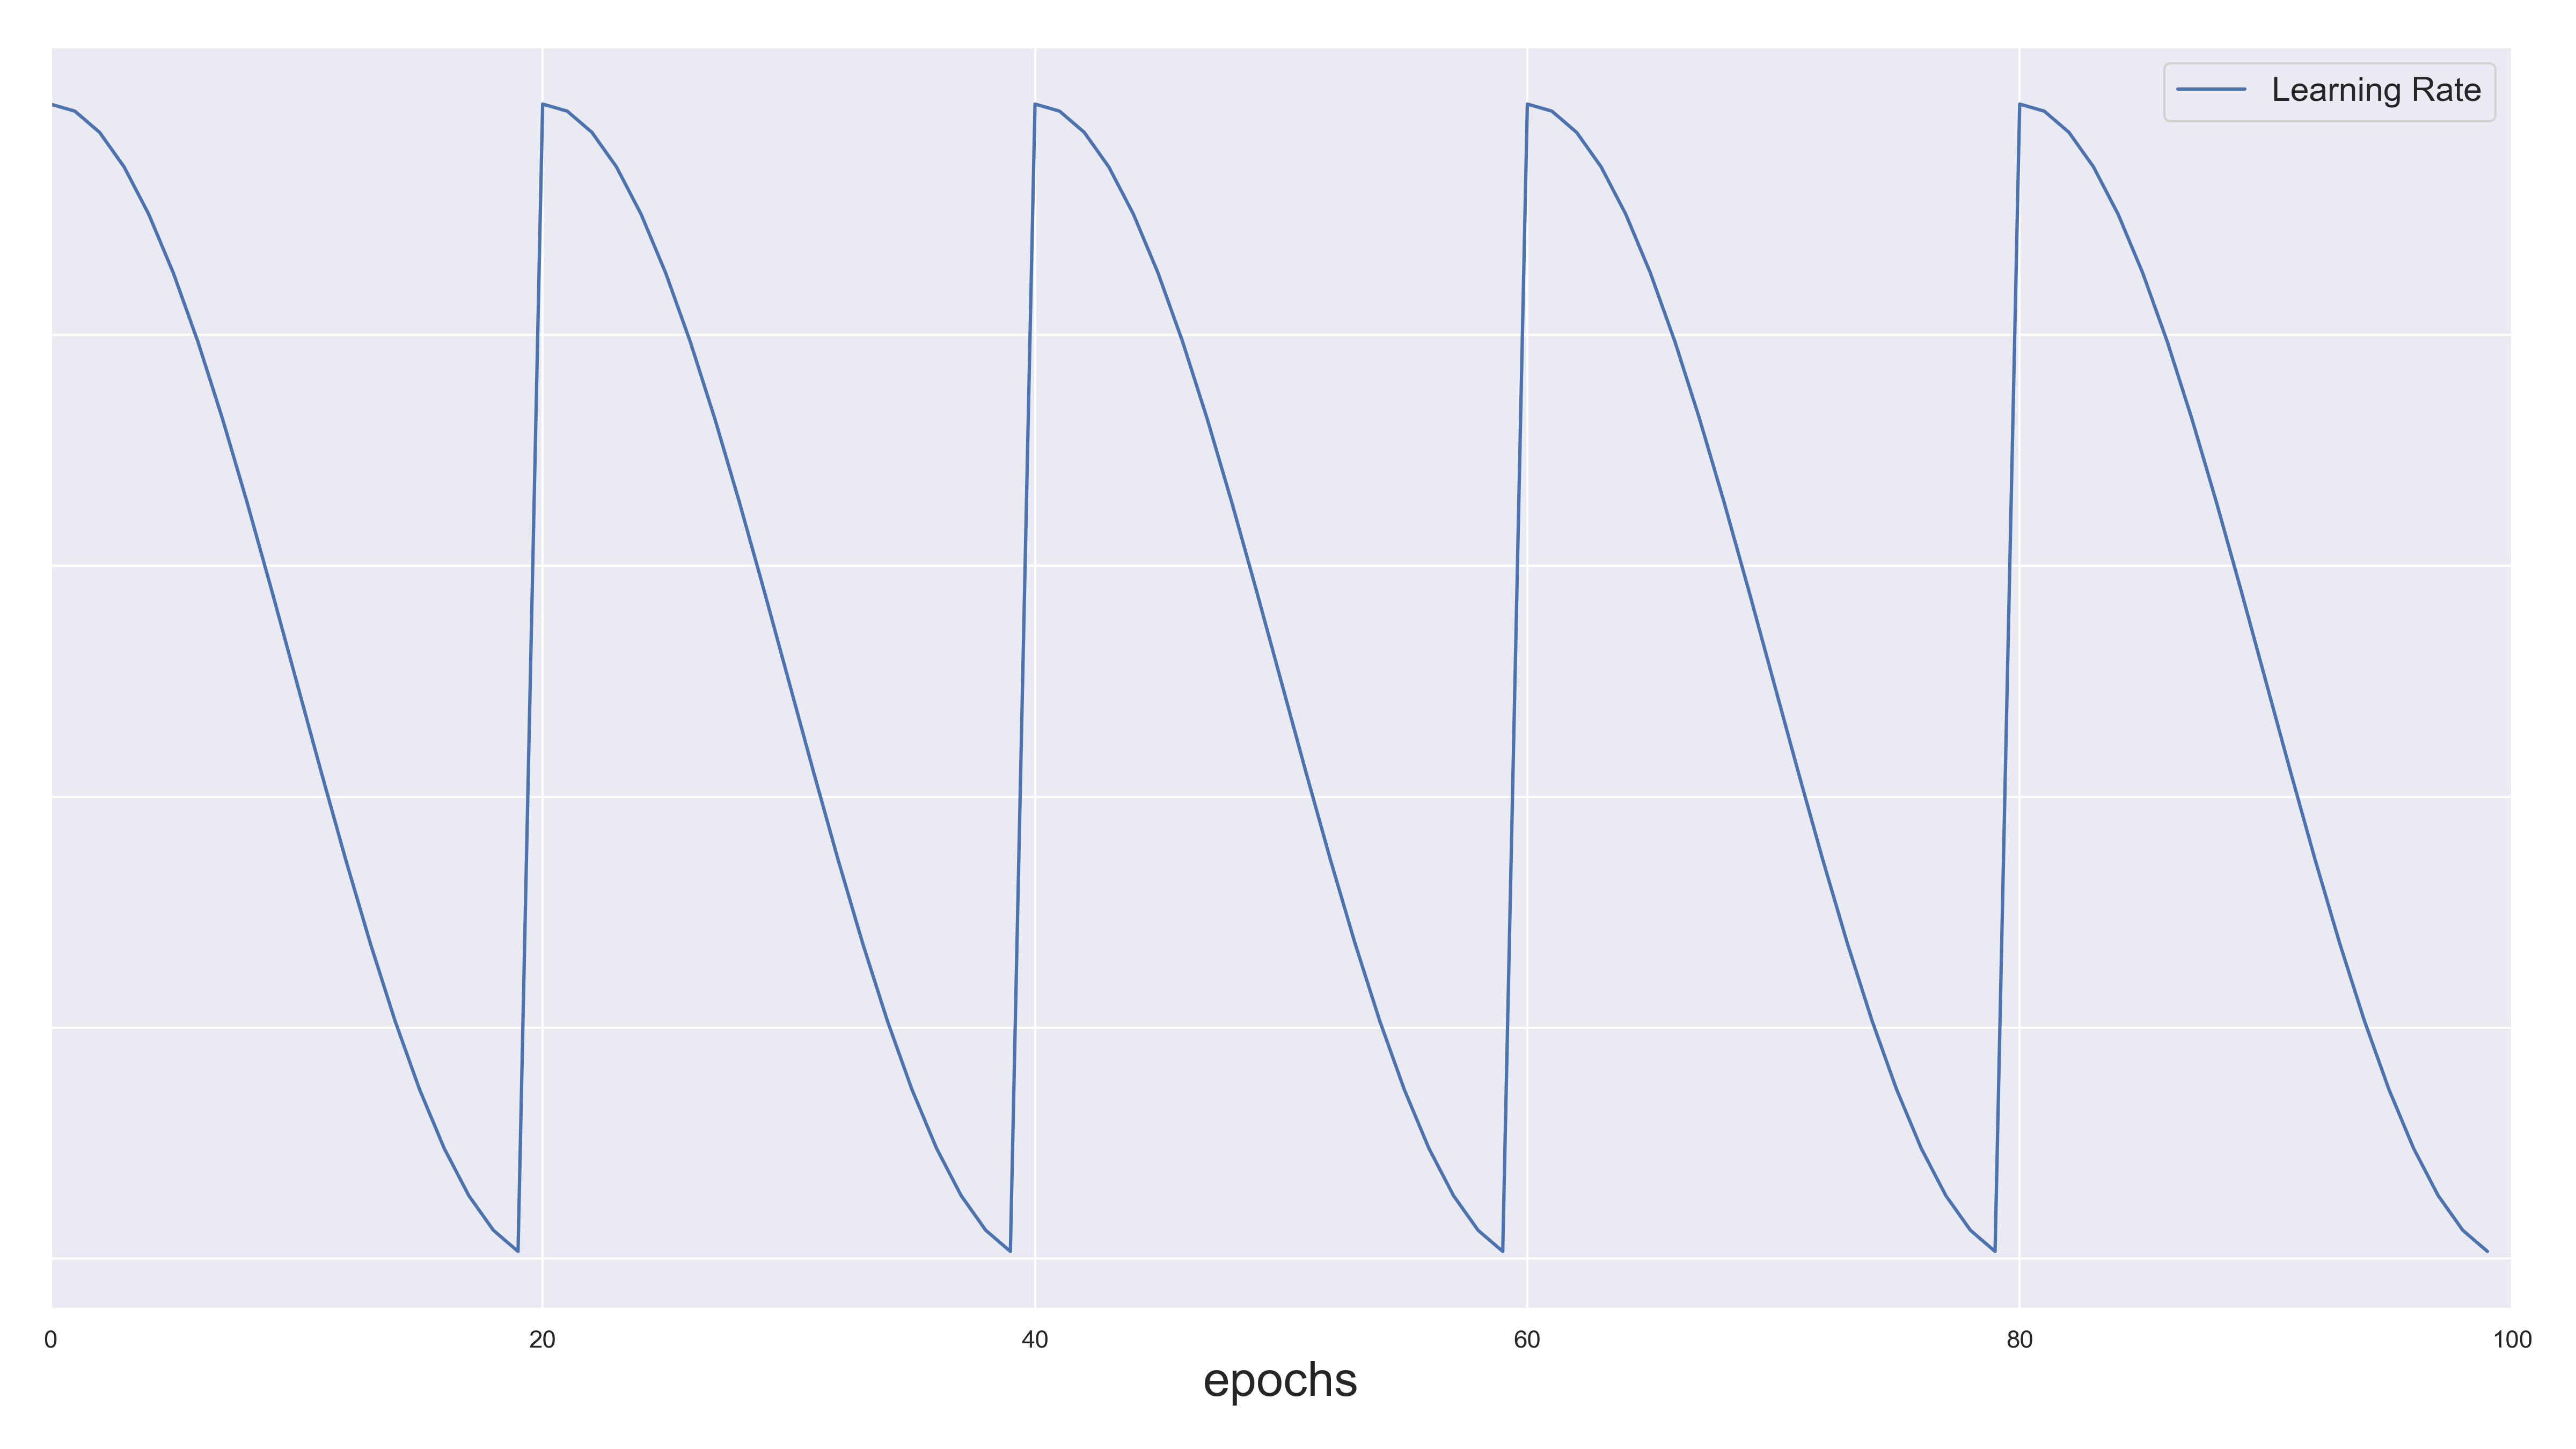
\includegraphics[width=.7\linewidth]{figures/lr.png}
			\captionof{figure}[Cosine Annealing Learning Rate]{Cosine Annealing Learning Rate} 
			\label{fig:cosineannealing}
		\end{minipage}
		
		\item[Batch Size] Batch Sizes between 1, and a few hundreds are recommended \cite{bengio_practical_2012}. To better utilize \gls{gpu}s, a batch size in the power of 2 gives better runtime, e.g., 32 to 256 \cite{goodfellow_deep_2016}. Advancements in parallelism \cite{dean_large_2012} have driven larger batch sizes, which can reduce the training time. However, smaller batch sizes have shown better generalization performance due to a regularizing effect \cite{masters_revisiting_nodate}. Especially large models that tend to overfit can benefit from smaller batch sizes \cite{goodfellow_deep_2016}. However, it results in increased training time.
		A batch size of 16 was found to be the maximum power of 2 possible within the computational budget of 8Gb RAM. The standard choice of 32 caused memory exhaustion. However, a batch size of 16 provide decent training times and may provide additional regularization over 32. Smaller batch sizes were not experimented with due to project scope.
		
		\item[Datasets] \gls{min100} is a subset of the \gls{ilsvrc2012} dataset \cite{russakovsky_imagenet_2015}. \gls{min100} was created for this project to reduce training time from several weeks to only days on available hardware. The subset is inspired by \cite{vinyals_matching_2016}, which also uses a subset of 100 classes with 600 samples for each class. \gls{min100} contains 100 out of 1.000 randomly sampled classes, which gives 127.300 out of 1.2m training samples, and 5.000 out of 50.000 validation samples. A full list of classes is found in table \ref{tbl:min100}. 
		
		Compared to other sufficiently dense classification datasets, e.g, \gls{tinyimagenet} \cite{li_cs231n:_2018}, \gls{cifar10} and \gls{cifar100} \cite{krizhevsky_cifar-10_nodate}, the image sizes of these datasets are respectively $(64\times 64$), $(32\times 32)$, $(32\times 32)$ pixels, all of which considered too small for this project. Other datasets such as MS COCO and Pascal VOC are better suited for object detection/segmentation, as images are not cropped to only focus on a single object, thus too challenging for classification. Pascal VOC was initially tested. However, training showed clear signs overfitted the training data due to data sparsity. 
		
		\item[Image Augmentation] Image augmentation is a tool to virtually create more training data \cite{perez_effectiveness_2017}, without having to annotate new samples \cite{goodfellow_deep_2016}. Image augmentation has shown to improve the validation accuracy as \gls{dnn}'s ability to generalize a specific classification problem has a close connection with the number of available training samples.
		Image augmentation involves transformations using tools from image processing to apply noise injection randomly or color space transformations, e.g., contrast and saturation distortions, geometric transformations, such as simple transformations of flipping the image, and affine transformations to create different image perspectives \cite{shorten_survey_2019}. Figure \ref{fig:augmentation} shows 64 random augmentations of an image of an elephant achieved using \gls{imgaug} \cite{jung_imgaug:_nodate}.  
		
		\begin{minipage}[t]{\linewidth}
			\centering
			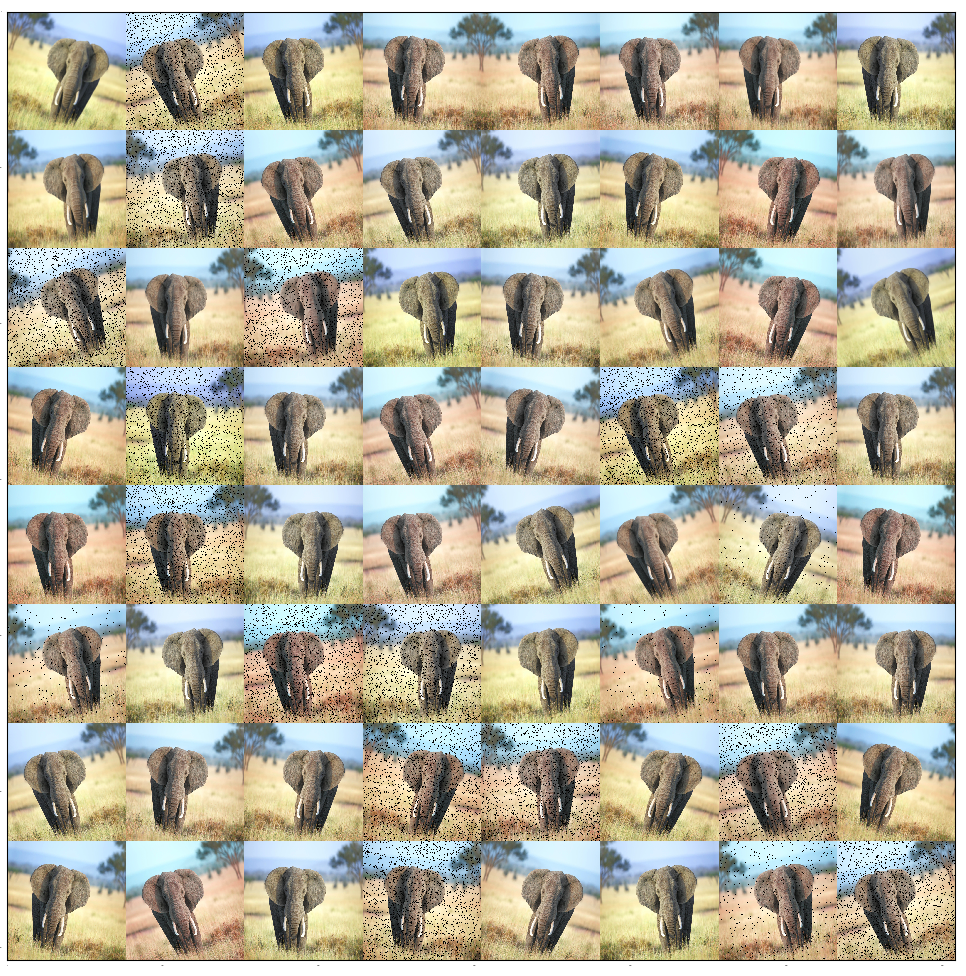
\includegraphics[width=.7\linewidth]{figures/augmentation/augmentation_high_resolution.png}
			\captionof{figure}[Image Augmentaion Example]{Image Augmentation of an elephant}
			\label{fig:augmentation}
		\end{minipage}
		
		New methods have been proposed where image transformations are learned to improve generalization, e.g., AutoAugment \cite{cubuk_autoaugment:_2018}. \gls{gan}s can help overcome the problem of limited data given the available training data or a 3D model, by artificially constructing synthetic samples in different backgrounds, light settings, and from alternate perspectives. However, these methods are another area of research and have been considered out of scope for this project.
		
		Methods that do not cover enriching the available training data, but alters the learning procedure are called regularization and covers; weight decay \cite{krogh_simple_nodate}, dropout \cite{srivastava_dropout:_nodate}, batch normalization \cite{ioffe_batch_2015}, and others. We do not experiment with these regularization techniques but use the settings already set in the implementation of the models.
		
		\item[Transfer Learning] Transfer learning is the procedure of using a pre-trained model to train on a new dataset. The assumption is that features learned on one image dataset can be reused for another dataset \cite{yosinski_how_2014}. Typically models have been pre-trained on the ImageNet dataset. The density of the dataset enables models to learn general features suitable for other domains \cite{kornblith_better_2019}. Transfer learning is especially suitable when the new data domain is of limited quantity, and the similarities between the two data domains are strong. If the similarities are weak, a model can be fine-tuned, i.e., only training the deep and specialized features. The general features of the shallow layers can be reused and are not optimized by freezing the weights \cite{li_cs231n:_2018}. Transfer learning can reduce the training time to learn general features of shallow layers, and possibly learn more specific features at deeper layers optimized for the new dataset.
	\end{enumdescript}
	
	\item[Inference]  All the hardware of table \ref{tbl:platforms} and all the trained models of table \ref{tbl:models} have been used. The inference experiment does not require nearly the same amount of settings as the training does. Those required are listed here:
	\begin{enumdescript}
		\item[Batch Size] A batch size of 1 have been chosen to simulate a realistic scenario and to measure time of each samples
		\item[Dataset] The validation dataset of \gls{min100} have been used, which contains 5000 samples.
	\end{enumdescript} 
	
\end{enumdescript}

\section{Results} \label{sec:ee-results}

The results section consists of two main parts. Section \ref{sec:ee-results-training} covers the result of training the \gls{dnn}s. Section \ref{sec:ee-results-inference} covers inference experimentation using our trained networks. 

\subsection{Training Results} \label{sec:ee-results-training}
We trained the three early exiting models \gls{bresnet}, \gls{bdensenet}, and \gls{msdnet}, along with conventional versions of the \gls{resnet}101 and \gls{densenet}-121.  In each epoch, the training loss and -accuracy and validation loss and -accuracy have been logged.
We trained \gls{bresnet} using transfer learning from the ImageNet dataset. We froze the features of the network. As in \cite{leroux_resource-constrained_2015}, we only trained the classifiers of the exits. Figure \ref{fig:frozen-b-resnet-miniimagenet-100} shows the results from of the training. The figure shows that none of the intermediate classifiers can obtain acceptable accuracy on neither the training nor the validation set. The features learned from a conventional model are not suitable for the early exit models. Because the features for the shallower part of the network are not optimized for the early classifiers. In \cite{teerapittayanon_branchynet:_2016}, they unfreeze the model base to allow the features of the model to be optimized for the intermediate classifiers of the early exits. Figure \ref{fig:b-resnet-miniimagenet-100} shows the training results with significant improvements. This study reveals the need to train the entire model to obtain an early exit model with decent accuracy.
\begin{center}
	
	\begin{minipage}[t]{.9\linewidth}
		
		\begin{figure}
			\centering
			\captionsetup[subfigure]{justification=centering, farskip=1pt,captionskip=1pt}
			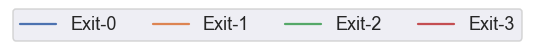
\includegraphics[width=.5\textwidth]{figures/training_plots/frozen_b-resnet_exit_legend}
			\subfloat[Train loss\label{fig:frozen-b-resnet-train-loss}]{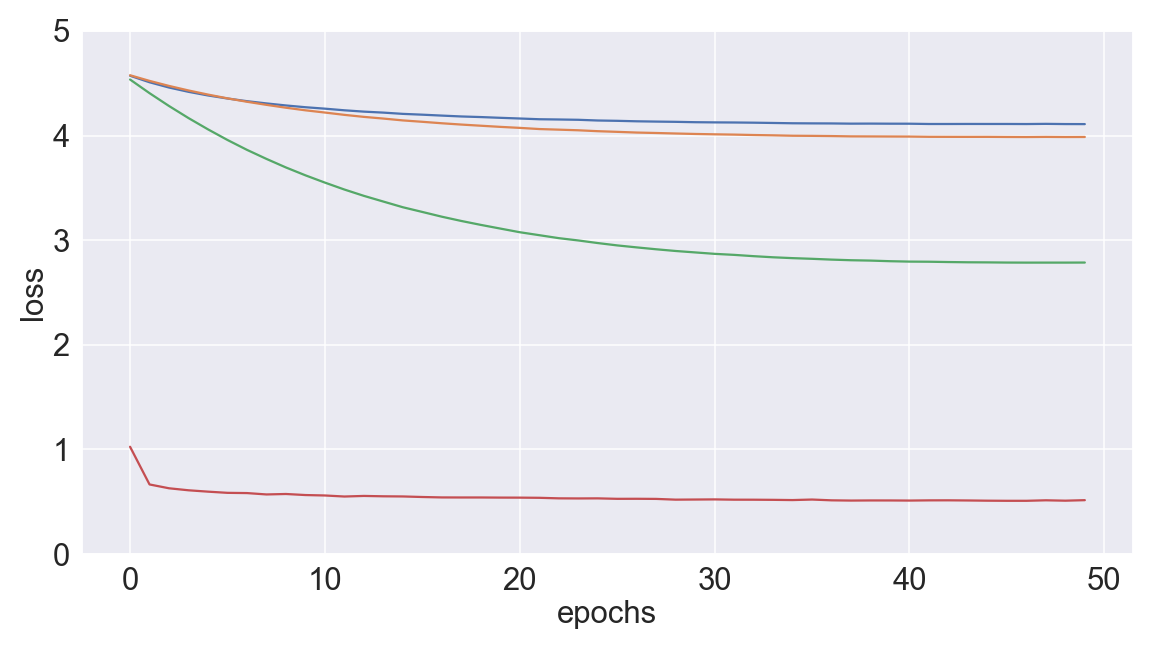
\includegraphics[width=.49\textwidth]{figures/training_plots/frozen_b-resnet_train-loss}}
			\subfloat[Test loss \label{fig:frozen-b-resnet-test-loss}]{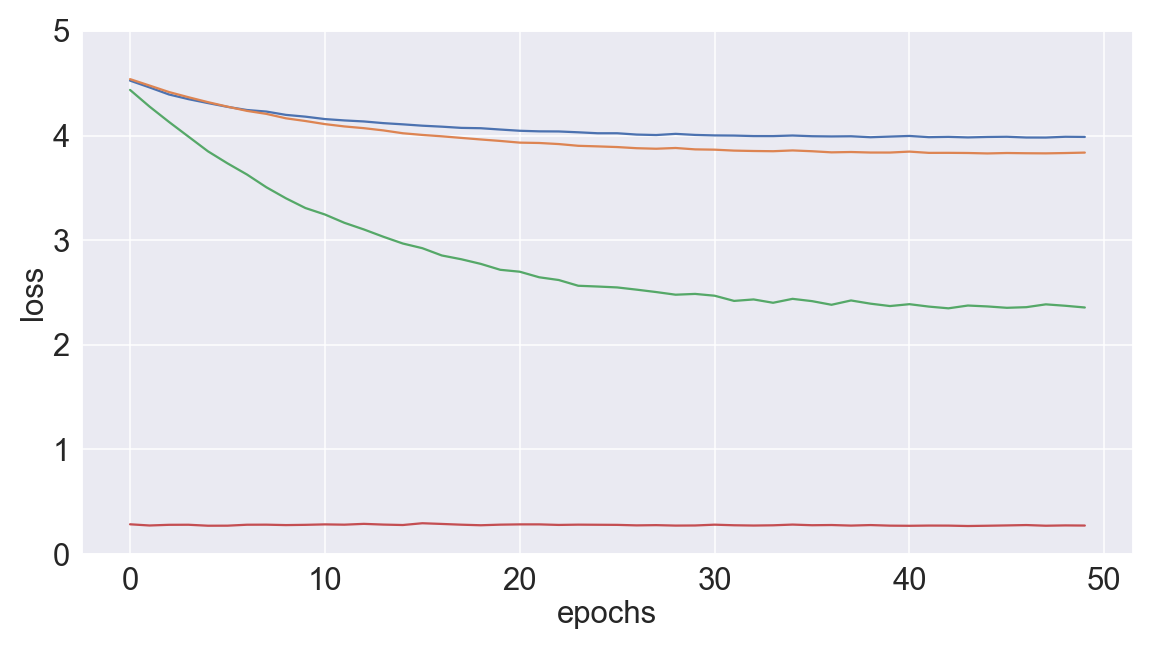
\includegraphics[width=.49\textwidth]{figures/training_plots/frozen_b-resnet_test-loss}}
			\hfill
			\subfloat[Train accuracy\label{fig:frozen-b-resnet-train-acc}]{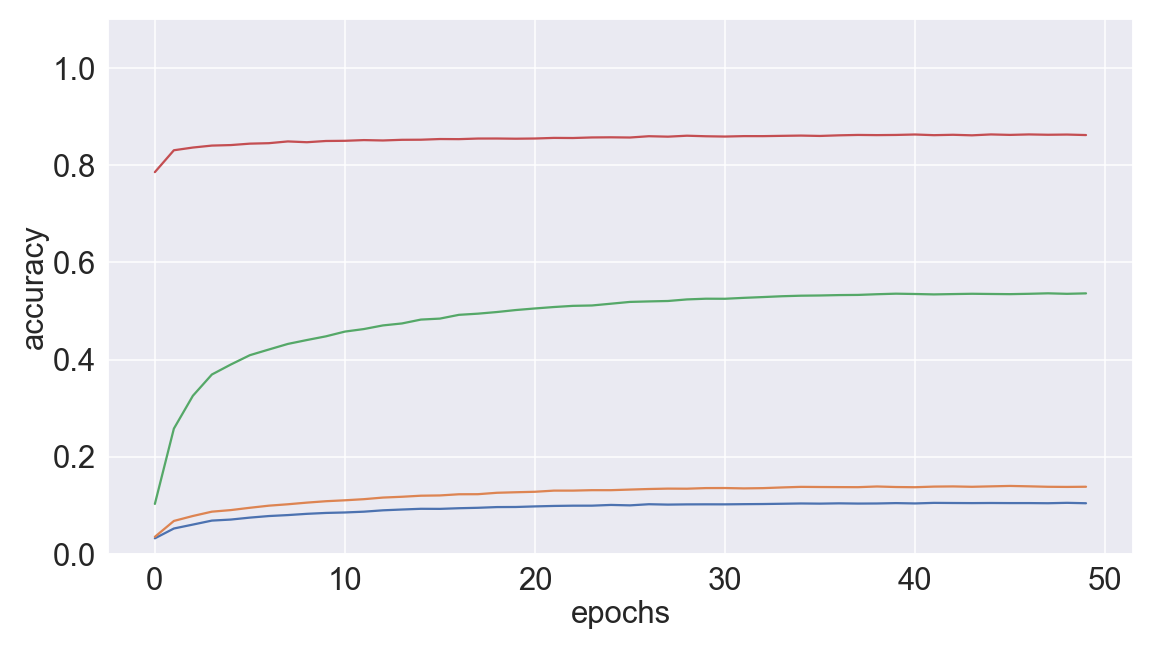
\includegraphics[width=.49\textwidth]{figures/training_plots/frozen_b-resnet_train-accuracy}}
			\subfloat[Test accuracy\label{fig:frozen-b-resnet-test-acc}]{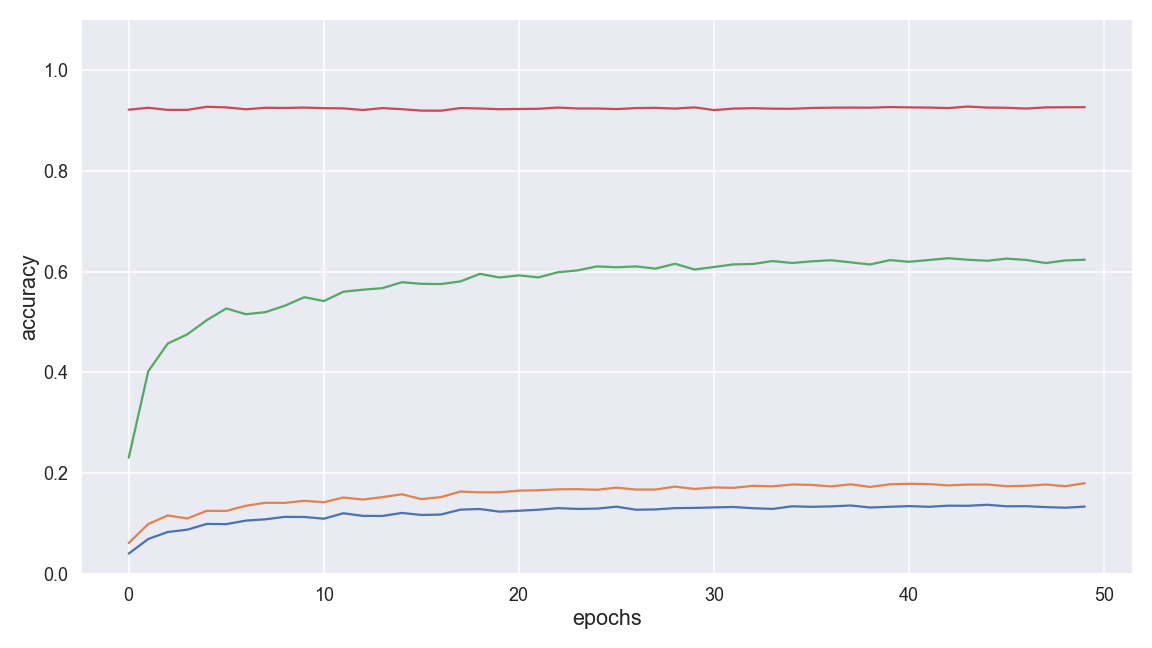
\includegraphics[width=.49\textwidth]{figures/training_plots/frozen_b-resnet_test-accuracy}}
			\caption[Frozen Bresnet Training summary]{Frozen \gls{bresnet} Training summary: shows the progression of model attributes over times of epochs, \protect\subref{fig:frozen-b-resnet-train-loss} train loss, \protect\subref{fig:frozen-b-resnet-test-loss} test loss, \protect\subref{fig:frozen-b-resnet-train-acc} train accuracy, \protect\subref{fig:frozen-b-resnet-test-acc}, test accuracy.}
			\label{fig:frozen-b-resnet-miniimagenet-100}
		\end{figure}
		\begin{figure}
			\centering
			\captionsetup[subfigure]{justification=centering, farskip=1pt,captionskip=1pt}
			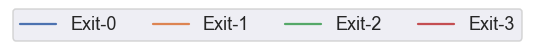
\includegraphics[width=.5\textwidth]{figures/training_plots/b-resnet_exit_legend}
			\subfloat[Train loss\label{fig:b-resnet-train-loss}]{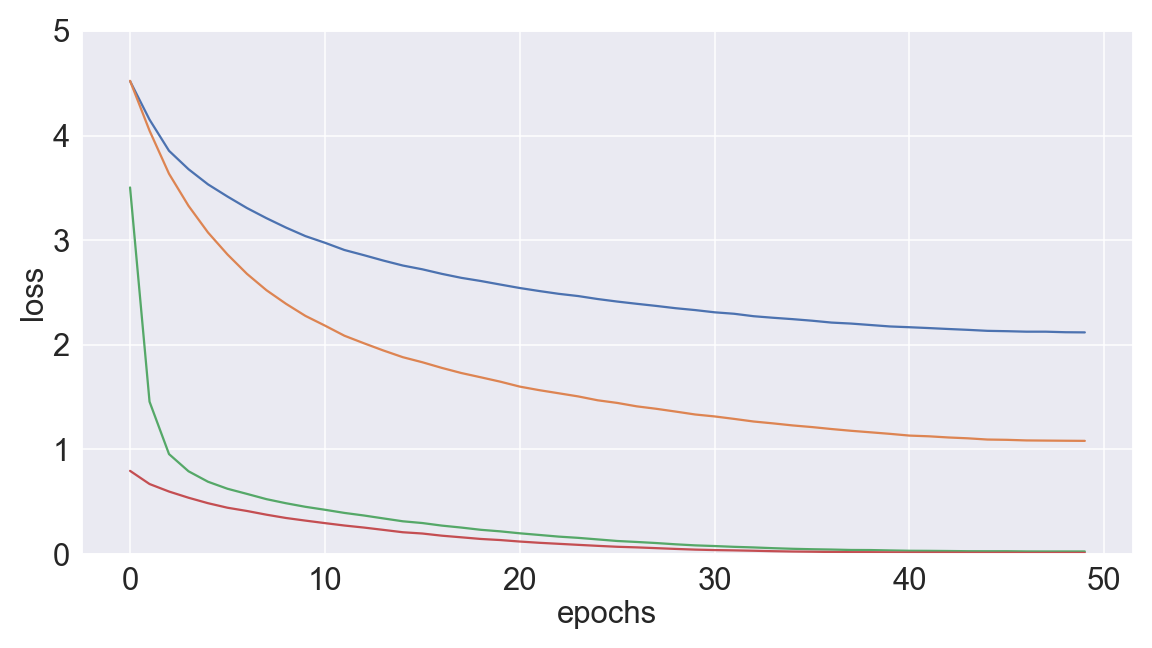
\includegraphics[width=.49\textwidth]{figures/training_plots/b-resnet_train-loss}}
			\subfloat[Test loss \label{fig:b-resnet-test-loss}]{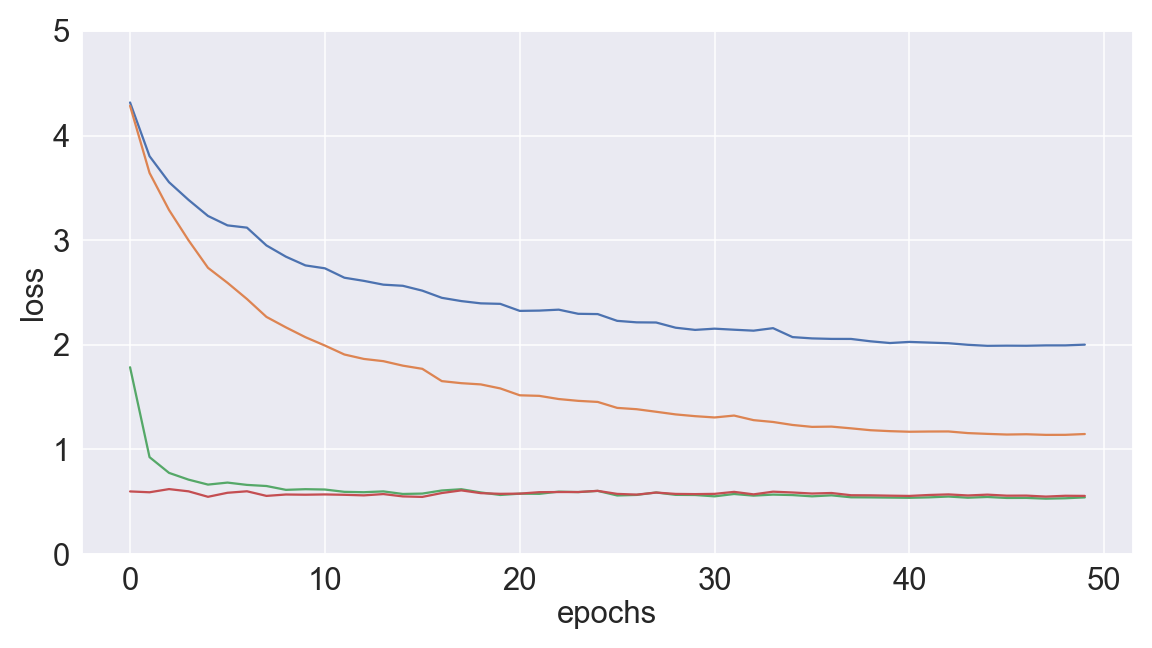
\includegraphics[width=.49\textwidth]{figures/training_plots/b-resnet_test-loss}}
			\hfill
			\subfloat[Train accuracy\label{fig:b-resnet-train-acc}]{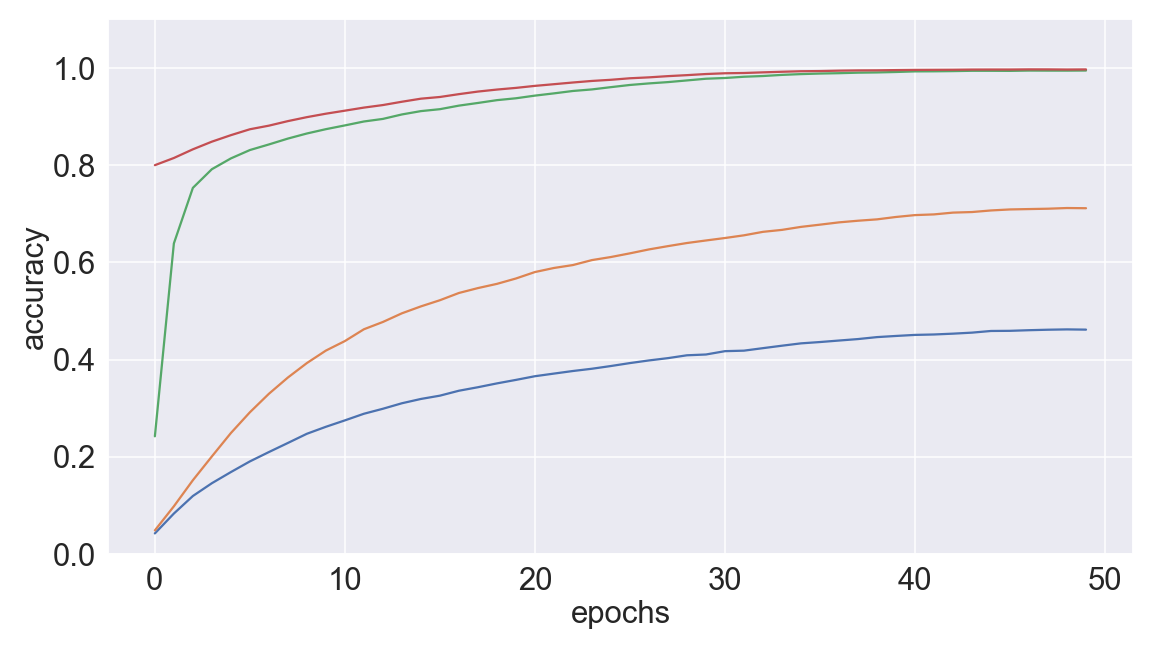
\includegraphics[width=.49\textwidth]{figures/training_plots/b-resnet_train-accuracy}}
			\subfloat[Test accuracy\label{fig:b-resnet-test-acc}]{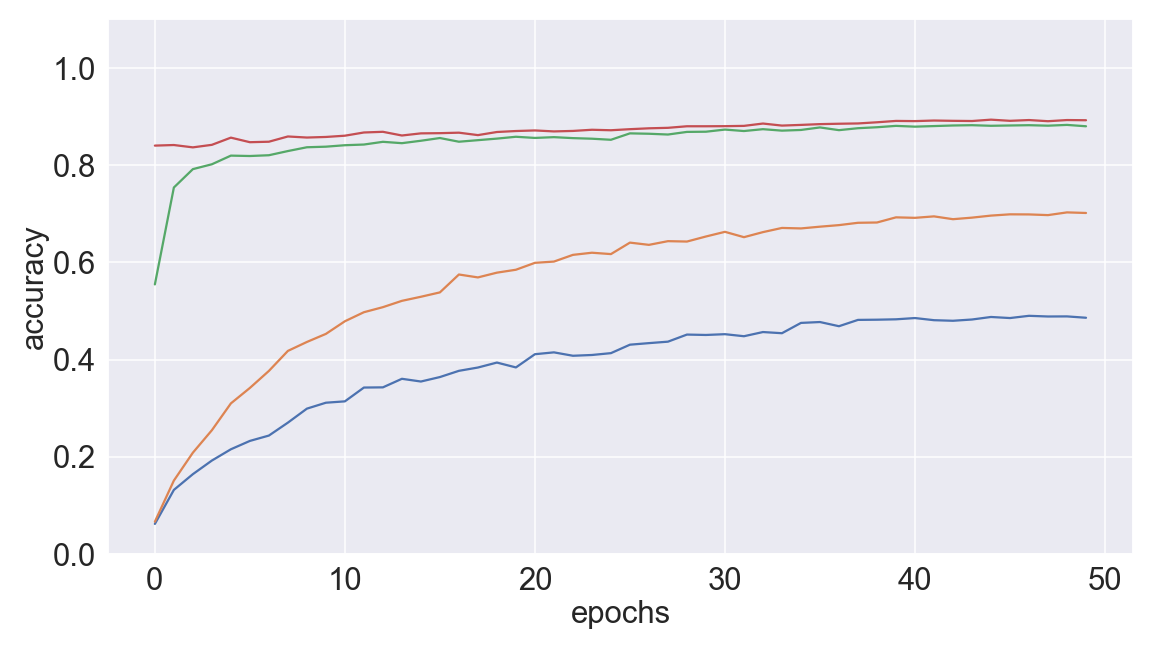
\includegraphics[width=.49\textwidth]{figures/training_plots/b-resnet_test-accuracy}}
			\caption[Unfrozen B-ResNet Training summary]{B-ResNet Training summary: shows the progression of model attributes over times of epochs, \protect\subref{fig:b-resnet-train-loss} train loss, \protect\subref{fig:b-resnet-test-loss} test loss, \protect\subref{fig:b-resnet-train-acc} train accuracy, \protect\subref{fig:b-resnet-test-acc}, test accuracy.}
			\label{fig:b-resnet-miniimagenet-100}
		\end{figure}
	\end{minipage}
\end{center}

Table \ref{tbl:frozen-vs-unfrozen} summarizes the validation accuracy. For each exit, we calculate the gain when training the entire model compared to a frozen base. The gain is most significant for the early exits as the features in the shallow layers now provide information that enables the early classifiers to discriminate the classes. 
\begin{longtabu}{>{\bfseries}X[2]|X[r]|X[r]|X[r]|X[r]}
	\caption[Comparison of Transfer Learning Approaches]{Comparison of transfer learning approaches frozen model vs. fine-tuning on validation accuracy} \label{tbl:frozen-vs-unfrozen} \\
	\toprule
	\rowfont{\bfseries}
	Model & Exit-0 & Exit-1 & Exit-2 & Exit-3 \tabularnewline
	\bottomrule
	\endfirsthead
	\multicolumn{3}{@{}l}{\textbf{\textcolor{black}{Table \ref{tbl:frozen-vs-unfrozen}:}} continued}\\
	\toprule
	\rowfont{\bfseries}
	Model & Exit-0 & Exit-1 & Exit-2 & Exit-1 \tabularnewline
	\bottomrule
	\endhead % all the lines above this will be repeated on every page
	\bottomrule
	\multicolumn{3}{@{}l}{continued \ldots}\\
	\endfoot
	\hline
	\endlastfoot
	Frozen B-\gls{resnet}	& 0.14	& 0.18	& 0.63 & 0.93 \tabularnewline
	\hline
	Unfrozen B-\gls{resnet}	& 0.49 	& 0.70 & 0.88 & 0.89 \tabularnewline
	\hline
	Gain & 3.50 & 3.89 & 1.40 &  0.96  \tabularnewline							
	\bottomrule
\end{longtabu}

The accuracy at early exits classifiers is greatly improved by 1.4 times to almost 3.9 times. However, the accuracy of the final classifier is reduced to 0.96 times. The reduction of accuracy may be caused by;
\begin{enumerate}
	\item The features of the third and largest resolution block (see table \ref{tbl:resnet101}) before exit-2, may become optimized too much for exit-2. Thus, it collapses the information that the last block needs to learn more descriptive features. 
	\item It could be a sign of overfitting due to the size of the dataset is only $\frac{1}{10}$ of the dataset used to train the original model. 
\end{enumerate}
However, the last two exits obtain a training accuracy close to 1. However, there is no notable degradation in validation loss or accuracy, which would have been the most definite sign of overfitting. We trained conventional versions of the two models on the same datasets, and since both models can obtain over 0.9 of accuracy. We argue that the most probable reason is optimization to earlier exit, as the same trend is shown in \cite{huang_multi-scale_2017}.
Henceforth we train the model without freezing the model base due to the significantly better results for the \gls{bresnet}. Figure \ref{fig:b-densenet-miniimagenet-100} shows the training result of B-\gls{densenet}. \gls{bdensenet} always has a gain in accuracy by continuing the inference process to the next exit, and is also able to achieve better accuracy at earlier exits than \gls{bresnet}. Figure \ref{fig:msdnet-miniimagenet-100} shows the results of training the \gls{msdnet}. Note, the \gls{msdnet} has five exits. The \gls{msdnet} is specially designed for early exiting and shows improvements for classifiers at early exits. However, the last two exits of \gls{bresnet} obtain superior accuracy compared to the other models. 
Note, none of the training sessions showed signs of overfitting, i.e., dropping train loss and rising test loss. If we continued the training, we could improve accuracy for the early exits. As already mentioned, we limited the number of epochs to 50 for all models due to time constraints and to fairly compare the model. 
\begin{center}
	\begin{minipage}[t]{.9\linewidth}
		
		\begin{figure}
			\centering
			\captionsetup[subfigure]{justification=centering, farskip=1pt,captionskip=1pt}
			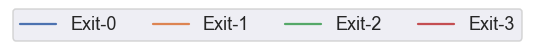
\includegraphics[width=.5\textwidth]{figures/training_plots/b-densenet_exit_legend}
			\subfloat[Train loss\label{fig:b-densenet-train-loss}]{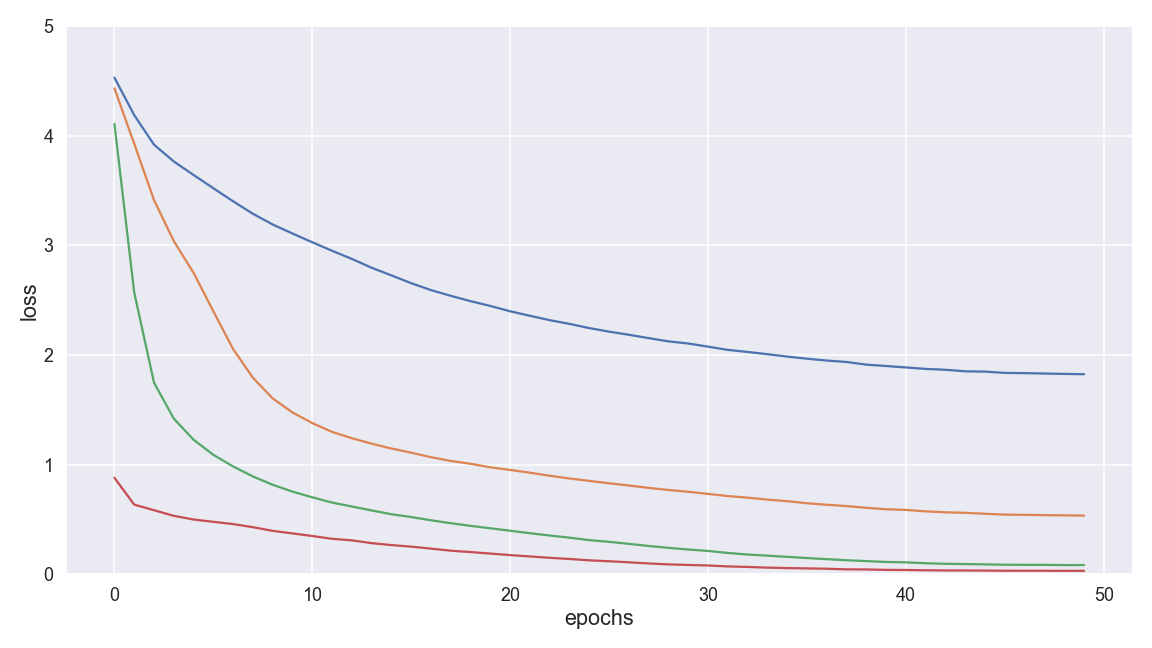
\includegraphics[width=.49\textwidth]{figures/training_plots/b-densenet_train-loss}}
			\subfloat[Test loss \label{fig:b-densenet-test-loss}]{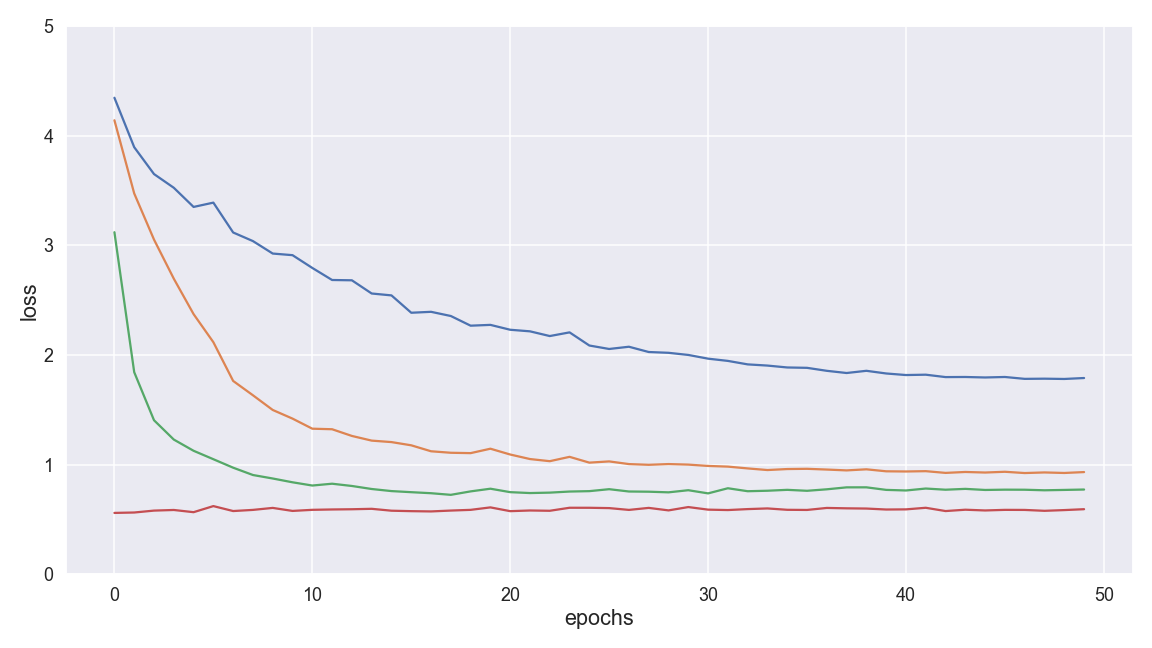
\includegraphics[width=.49\textwidth]{figures/training_plots/b-densenet_test-loss}}
			\hfill
			\subfloat[Train accuracy\label{fig:b-densenet-train-acc}]{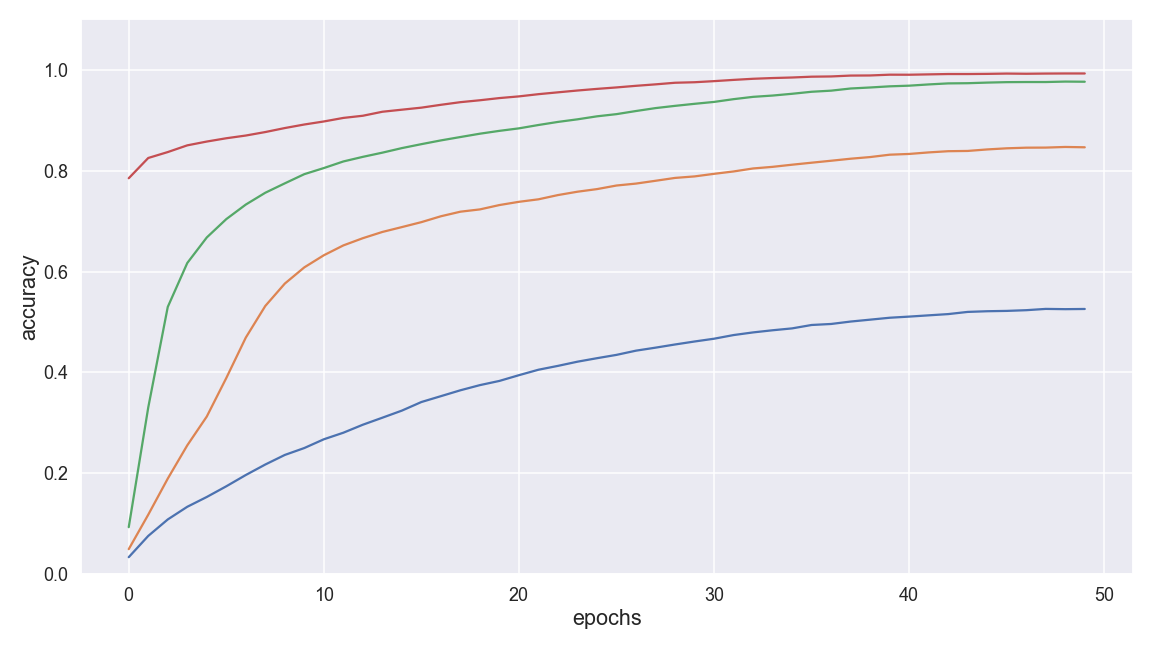
\includegraphics[width=.49\textwidth]{figures/training_plots/b-densenet_train-accuracy}}
			\subfloat[Test accuracy\label{fig:b-densenet-test-acc}]{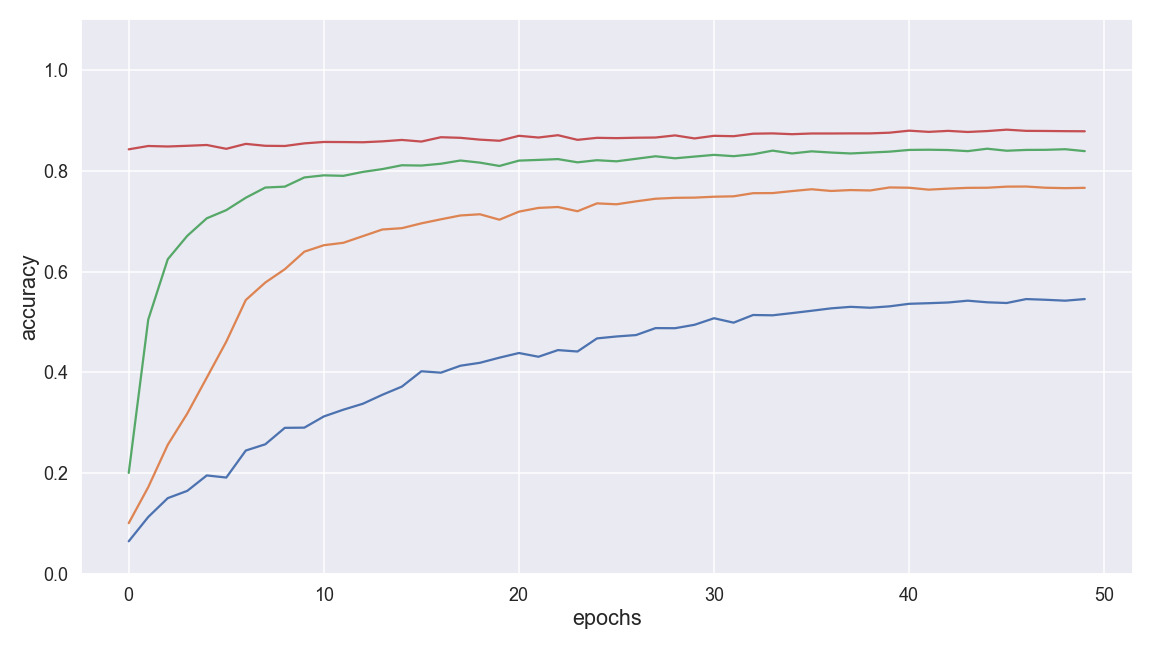
\includegraphics[width=.49\textwidth]{figures/training_plots/b-densenet_test-accuracy}}
			\caption[B-densenet Training summary]{B-densenet Training summary: shows the progression of model attributes over times of epochs, \protect\subref{fig:b-densenet-train-loss} train loss, \protect\subref{fig:b-densenet-test-loss} test loss, \protect\subref{fig:b-densenet-train-acc} train accuracy, \protect\subref{fig:b-densenet-test-acc}, test accuracy.}
			\label{fig:b-densenet-miniimagenet-100}
		\end{figure}
		
		\begin{figure}
			\centering
			\captionsetup[subfigure]{justification=centering, farskip=1pt,captionskip=1pt}
			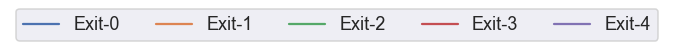
\includegraphics[width=.5\textwidth]{figures/training_plots/msdnet_exit_legend}
			\subfloat[Train loss\label{fig:msdnet-train-loss}]{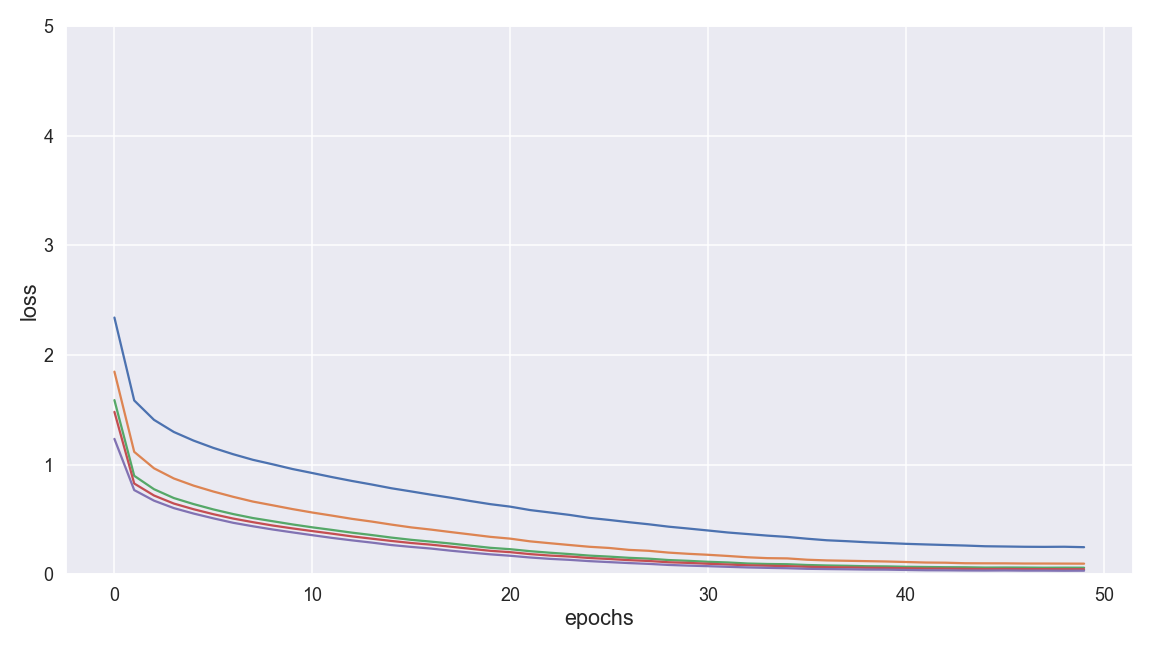
\includegraphics[width=.49\textwidth]{figures/training_plots/msdnet_train-loss}}
			\subfloat[Test loss \label{fig:msdnet-test-loss}]{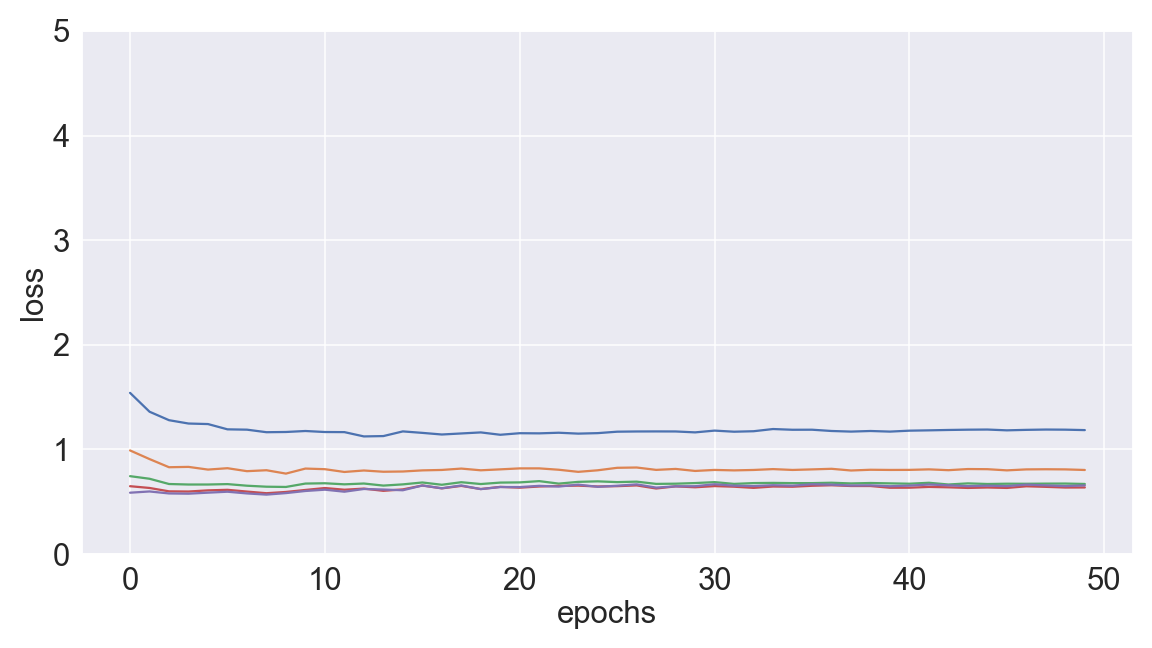
\includegraphics[width=.49\textwidth]{figures/training_plots/msdnet_test-loss}}
			\hfill
			\subfloat[Train accuracy\label{fig:msdnet-train-acc}]{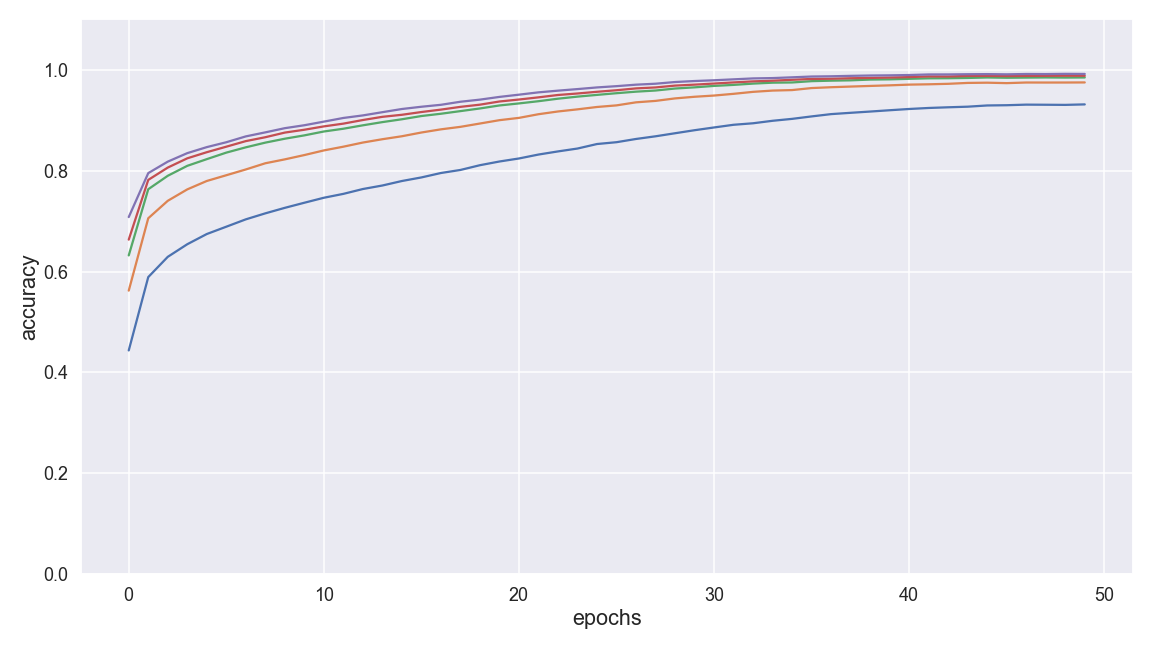
\includegraphics[width=.49\textwidth]{figures/training_plots/msdnet_train-accuracy}}
			\subfloat[Test accuracy\label{fig:msdnet-test-acc}]{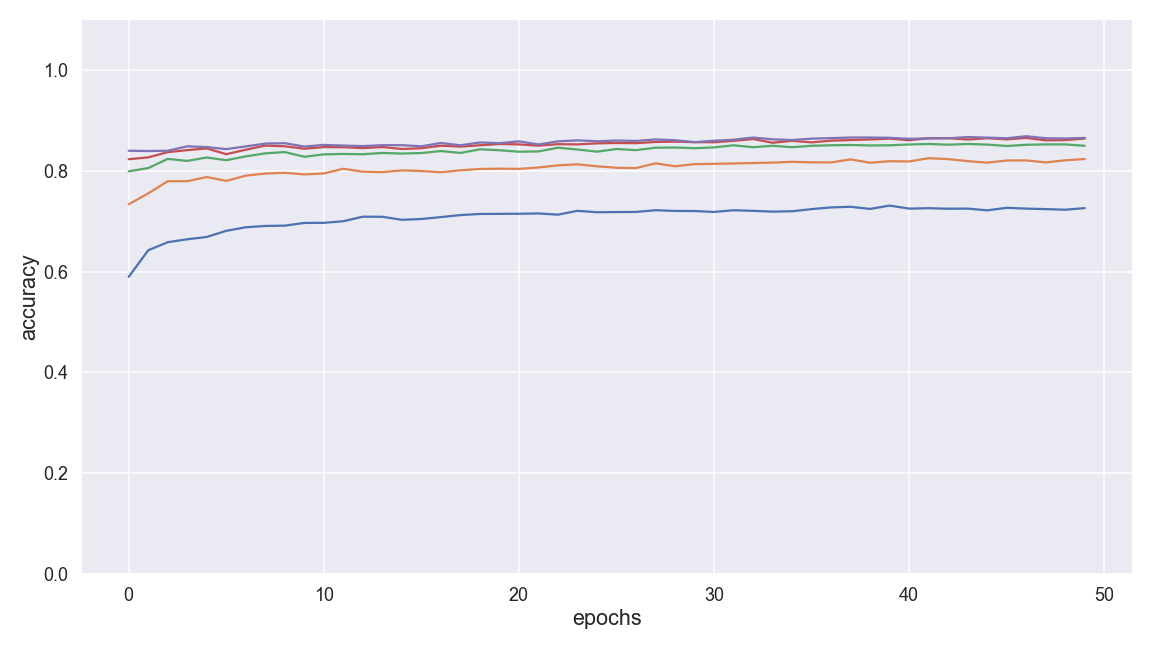
\includegraphics[width=.49\textwidth]{figures/training_plots/msdnet_test-accuracy}}
			\caption[MSDNet Training summary]{MSDNet Training summary: shows the progression of model attributes over times of epochs, \protect\subref{fig:msdnet-train-loss} train loss, \protect\subref{fig:msdnet-test-loss} test loss, \protect\subref{fig:msdnet-train-acc} train accuracy, \protect\subref{fig:msdnet-test-acc}, test accuracy.}
			\label{fig:msdnet-miniimagenet-100}
		\end{figure}
	\end{minipage}
\end{center}

\subsection{Inference Results} \label{sec:ee-results-inference}

In this section, we evaluate the accuracy of the early exit models. All validation samples are inferred to all models of table \ref{tbl:models}. Figure \ref{fig:exit-accuracy} shows the top-1 and top-5 accuracy of all exits of the three models.  The models achieve higher accuracy at deeper exits in the network, as the increasingly complex features deep within the networks have more discriminative characteristics; hence the classifiers achieve better performance. Table \ref{tbl:validation-comparison} compares the top-1 accuracy  of the three models
\begin{figure}
	\centering
	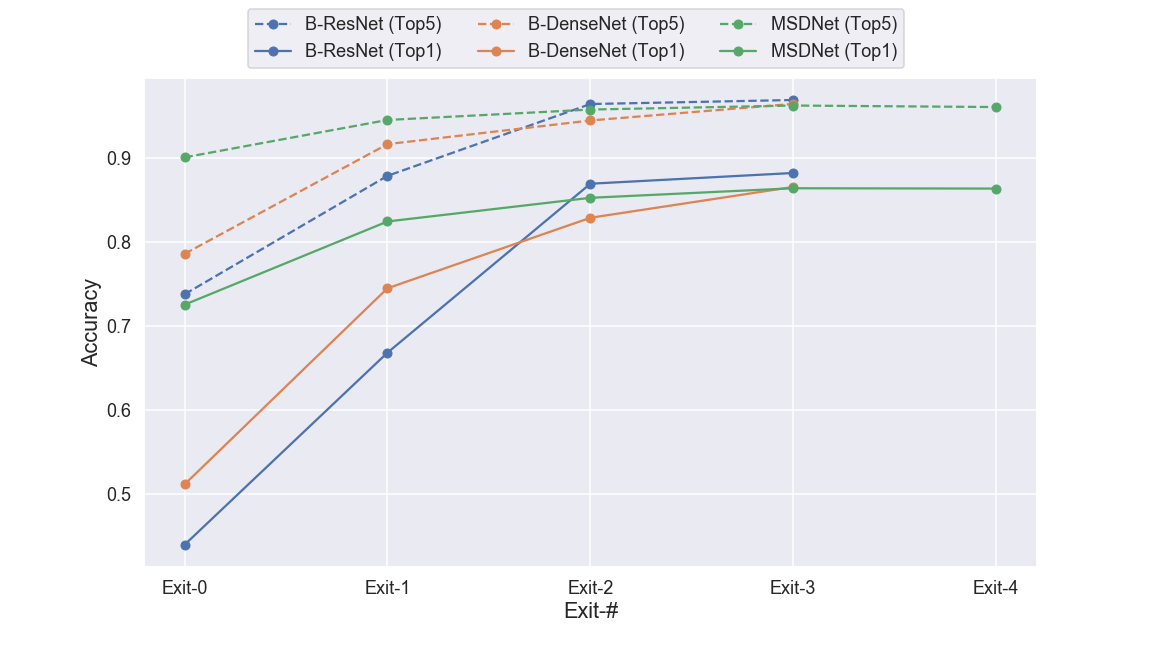
\includegraphics[width=.8\linewidth]{figures/inference_plots/accuracy-comparison}
	\caption[Accuracy of Early Exit Models]{Accuracy of Early Exit Models, B-\gls{resnet}, B-\gls{densenet}, and \gls{msdnet}}
	\label{fig:exit-accuracy}
\end{figure}


\begin{longtabu}{>{\bfseries}X[2]|X|X|X|X|X}
	\caption[Early Exiting Top-1 Accuracy]{Early Exiting Validation Accuracy} \label{tbl:validation-comparison} \\
	\toprule
	\rowfont{\bfseries}
	Model & Exit-0 & Exit-1 & Exit-2 & Exit-3 & Exit-4 \tabularnewline
	\bottomrule
	\endfirsthead
	\multicolumn{3}{@{}l}{\textbf{\textcolor{black}{Table \ref{tbl:frozen-vs-unfrozen}:}} continued}\\
	\toprule
	\rowfont{\bfseries}
	Model & Exit-0 & Exit-1 & Exit-2 & Exit-3 & Exit-4 \tabularnewline
	\bottomrule
	\endhead % all the lines above this will be repeated on every page
	\bottomrule
	\multicolumn{3}{@{}l}{continued \ldots}\\
	\endfoot
	\hline
	\endlastfoot
	B-\gls{resnet} & 0.49 	& 0.70 & 0.88 & 0.89 & N/A \tabularnewline
	\hline
	B-\gls{densenet}	& 0.55 	& 0.77 & 0.84 & 0.88 & N/A \tabularnewline
	\hline
	\gls{msdnet} & 0.73 & 0.82 & 0.85 &  0.87 & 0.87 \tabularnewline							
	\bottomrule
\end{longtabu}

Promisingly close to 50 \% of the samples can be accurately classified at the first exit of any of the early exit models. Table \ref{tbl:validation-comparison} shows the importance of the densely connected layers for an early exit model, as found in \cite{huang_multi-scale_2017}.  The higher accuracy for early exits in both \gls{bdensenet} and \gls{msdnet} compared to the lower accuracy of \gls{bresnet} substantiates this claim. However, the end-exit of \gls{bresnet} achieves superior top-1 accuracy compared to the other models. The two last exits of \gls{bresnet} is almost equally accurate; not much gain is obtained by running the inference to the end.  
\subsubsection{Inference Time Analysis}
We infer the validation data and measure the inference time for each exit of all five models on the three platforms. Table \ref{tbl:inference-stats} shows the mean, standard deviation, minimum, and maximum for the model inference time on the platforms. The early exit framework only adds a small delay overhead from the early exit classifiers, when comparing the last exit runtimes of the \gls{branchynet} models, with its conventional counterpart. For the \gls{gpu}-enabled platforms, \gls{gpu} Workstation Jetson TX2, a small average delay overhead of 1.1 ms and 2.4 ms respectively for the two platforms. On the \gls{nuc}, the overhead the \gls{bresnet} is  7.5 ms slower than \gls{resnet}. However, the \gls{densenet} is only slightly slower than \gls{densenet} by 0.01 ms.   
\begin{footnotesize}
	\begin{longtabu}{>{\bfseries}X[2.6]|[1pt]X[r]|X[0.8r]|X[r]|X[1.2r]|[1pt]X[r]|X[0.7r]|X[r]|X[1.2r]|[1pt]X[r]|X[0.7r]|X[r]|X[1.2r]}
		\caption[Inference time statistics]{Inference time statistics (mean, standard deviation, minimum, maximum) of the five models on the three platforms }\label{tbl:inference-stats} \\
		\toprule
		\rowfont{\bfseries}
		& \multicolumn4{c|[1pt]}{GPU Workstation (ms)} &  \multicolumn4{c|[1pt]}{Jetson TX2 (ms)} & \multicolumn4{c}{Intel NUC (ms)} \tabularnewline
		\tabucline{2-13}
		\rowfont{\bfseries} Model & Mean & Std.  & Min & Max & Mean & Std. & Min & Max & Mean & Std.  & Min & Max  \tabularnewline
		\hline
		\endfirsthead
		\multicolumn{3}{@{}l}{\textbf{\textcolor{black}{Table \ref{tbl:inference-stats}:}} continued}\\
		\toprule
		\rowfont{\bfseries}
		& \multicolumn4{c|[1pt]}{GPU Workstation (ms)} &  \multicolumn4{c|[1pt]}{Jetson TX2 (ms)} & \multicolumn4{c}{Intel NUC (ms)} \tabularnewline
		\tabucline{2-13}
		\rowfont{\bfseries} Model & Mean & Std.  & Min & Max & Mean & Std.  & Min & Max & Mean & Std.  & Min & Max  \tabularnewline
		\hline
		\endhead % all the lines above this will be repeated on every page
		\hline
		\multicolumn{3}{@{}l}{continued \ldots}\\
		\endfoot
		\hline
		\endlastfoot
		ResNet  	& 36.01 & 1.72 & 33.24 & 69.02 & 64.19 & 1.95 & 61.28 & 110.17 & 215.76 & 21.98 & 132.98 & 275.55 \tabularnewline
		\hline
		DenseNet 	& 47.74 & 1.95 & 4.48 & 86.88 & 70.48 & 3.04 & 59.56 & 132.45 &  72.30 &  2.61 &  69.02 & 107.63 \tabularnewline
		\hline
		B-ResNet & & & &&&&&&&& &  \tabularnewline 
		\hspace{3mm} Exit-0 &  4.20 & 0.63 &  3.81 &  39.40 &  8.61 & 0.31 &  8.39 &  15.54 &  38.25 &  1.85 &  29.26 &  74.94 \tabularnewline
		\hspace{3mm} Exit-1 &  9.40 & 1.28 &  8.19 &  70.23 & 19.30 & 1.08 & 16.42 &  38.41 &  66.69 &  3.15 &  50.41 & 110.80 \tabularnewline
		\hspace{3mm} Exit-2 & 33.59 & 2.78 & 30.25 & 103.55 & 56.77 & 2.73 & 52.34 & 102.58 & 196.43 &  8.81 & 150.11 & 254.86 \tabularnewline
		\hspace{3mm} Exit-3 & 37.14 & 2.94 & 33.65 & 109.94 & 67.04 & 2.86 & 62.47 & 116.74 & 223.32 & 10.35 & 170.95 & 289.67 \tabularnewline
		\hline
		B-DenseNet &  & & &&&&&&&& & \tabularnewline
		\hspace{3mm} Exit-0 &  5.83 & 1.09 &  5.15 &  54.61 & 11.05 & 0.48 & 10.52 & 17.31 &  28.83 & 1.59 & 26.05 & 41.93 \tabularnewline
		\hspace{3mm} Exit-1 & 17.03 & 1.89 & 14.60 &  76.78 & 30.26 & 2.02 & 23.75 & 47.54 &  46.71 & 2.31 & 43.47 & 71.85 \tabularnewline
		\hspace{3mm} Exit-2 & 36.31 & 3.01 & 32.72 & 104.79 & 55.38 & 3.22 & 48.10 & 87.81 &  64.26 & 2.80 & 60.65 & 99.41 \tabularnewline
		\hspace{3mm} Exit-3 & 49.14 & 3.36 & 45.13 & 127.07 & 72.41 & 3.89 & 64.77 & 120.29 & 72.31 & 2.97 & 68.37 & 112.06 \tabularnewline
		\hline
		MSDNet & & &&&&&&&&&& \tabularnewline
		\hspace{3mm} Exit-0 & 24.14 & 1.59 & 21.53 &  67.38 &  40.37 & 2.77 & 29.36 & 209.89 & 19.99 & 1.27 & 16.99 &  35.12 \tabularnewline
		\hspace{3mm} Exit-1 & 42.24 & 2.54 & 38.87 & 119.85 &  65.18 & 4.29 & 53.34 & 267.19 & 32.82 & 2.38 & 29.03 & 103.19 \tabularnewline
		\hspace{3mm} Exit-2 & 55.59 & 2.82 & 51.90 & 143.30 &  83.81 & 5.43 & 71.39 & 312.55 & 42.89 & 3.03 & 38.72 & 130.52 \tabularnewline
		\hspace{3mm} Exit-3 & 64.49 & 2.99 & 60.59 & 156.26 &  96.53 & 6.26 & 83.68 & 345.67 & 50.10 & 3.43 & 45.66 & 145.75 \tabularnewline
		\hspace{3mm} Exit-4 & 68.87 & 3.11 & 64.85 & 165.90 & 103.29 & 6.65 & 90.14 & 361.02 & 56.02 & 3.62 & 51.28 & 154.08 \tabularnewline
		\bottomrule
	\end{longtabu}
	
\end{footnotesize}

The inference times are very different on the three platforms. The inference time is dependent on the hardware. The \gls{bresnet} achieves decent runtime utilizing a \gls{gpu}, whereas \gls{bdensenet} achieves decent runtime in either case. In general, the \gls{gpu-ws} is the fastest due to the larger \gls{gpu} with more parallelization capabilities. Especially the \gls{resnet}-based models achieve far superior runtimes on this platform. The \gls{nuc} is generally the slowest except for the \gls{msdnet}; it achieves runtime competitive with \gls{resnet}-based model on the \gls{gpu-ws}. Figure \ref{fig:inference-time-dist} shows the distribution of runtime used at each exit.

\begin{figure}
	\begin{minipage}{\textwidth}
		\centering
		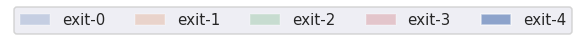
\includegraphics[width=.5\linewidth]{figures/inference_plots/time_dist_legend}
	\end{minipage}
	\begin{minipage}{0.33\textwidth}
		\captionsetup[subfigure]{farskip=0pt,captionskip=0pt, justification=centering}
		\centering
		GPU Workstation
		\subfloat[\gls{resnet} ]{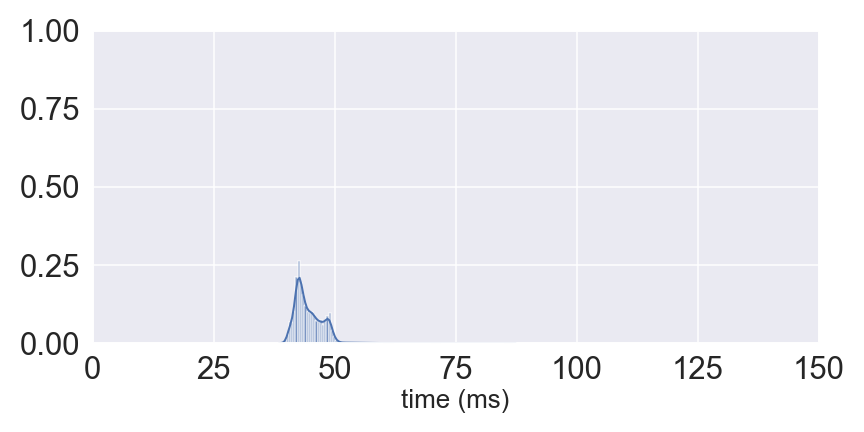
\includegraphics[width=\textwidth,height=.2\textheight,keepaspectratio]{figures/inference_plots/gpu_resnet_inference_time_distribution}}
		\hfill
		\subfloat[B-\gls{resnet}]{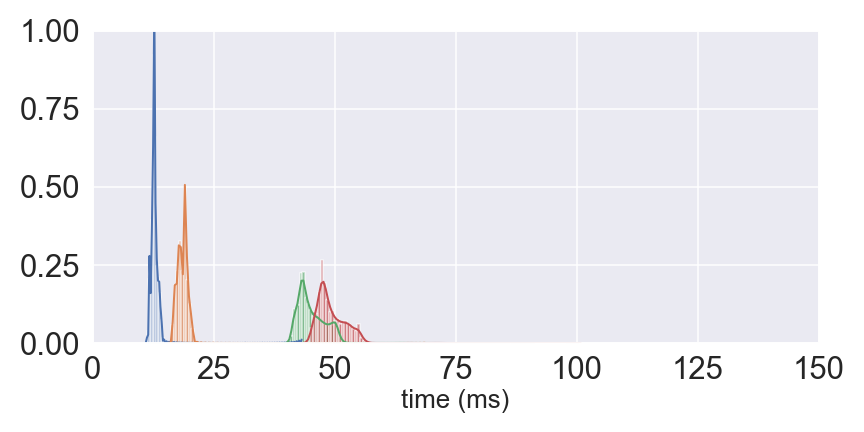
\includegraphics[width=\textwidth,height=.2\textheight,keepaspectratio]{figures/inference_plots/gpu_b-resnet_inference_time_distribution}}
		\hfill
		\subfloat[\gls{densenet} ]{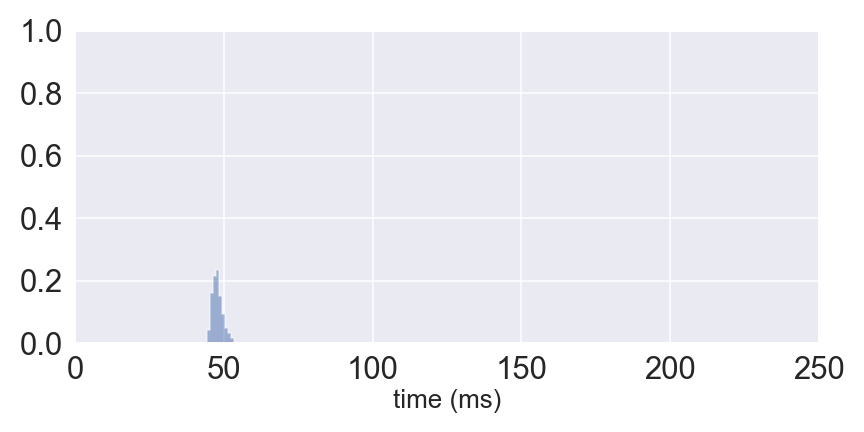
\includegraphics[width=\textwidth,height=.2\textheight,keepaspectratio]{figures/inference_plots/gpu_densenet_inference_time_distribution}}
		\hfill
		\subfloat[B-\gls{densenet}]{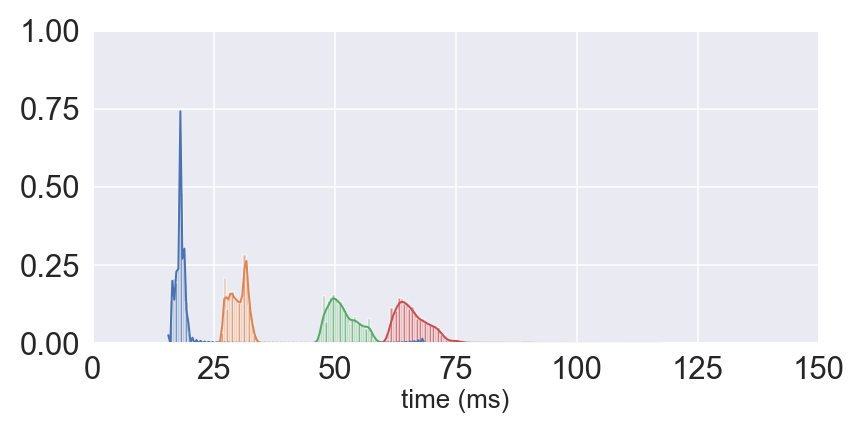
\includegraphics[width=\textwidth,height=.2\textheight,keepaspectratio]{figures/inference_plots/gpu_b-densenet_inference_time_distribution}}
		\hfill
		\subfloat[\gls{msdnet}]{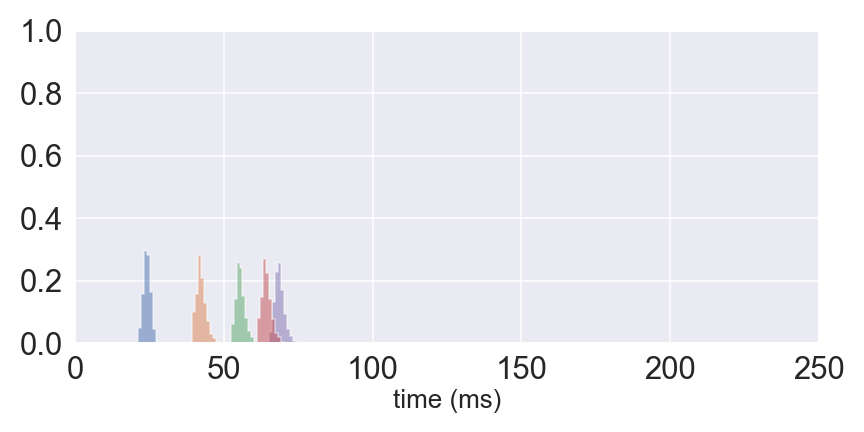
\includegraphics[width=\textwidth,height=.2\textheight,keepaspectratio]{figures/inference_plots/gpu_msdnet_inference_time_distribution}}
	\end{minipage}
	\begin{minipage}{0.33\textwidth}
		\captionsetup[subfigure]{farskip=0pt,captionskip=0pt,justification=centering}
		\centering
		Jetson TX2
		\subfloat[\gls{resnet} ]{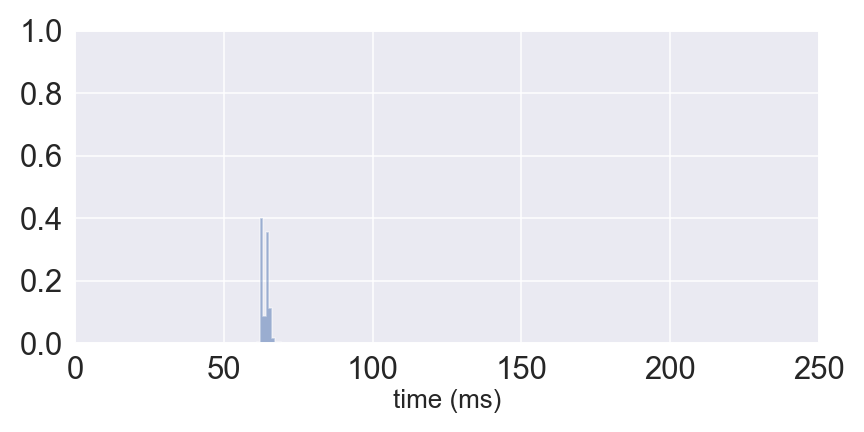
\includegraphics[width=\textwidth,height=.2\textheight,keepaspectratio]{figures/inference_plots/jetson_resnet_inference_time_distribution}}
		\hfill
		\subfloat[B-\gls{resnet}]{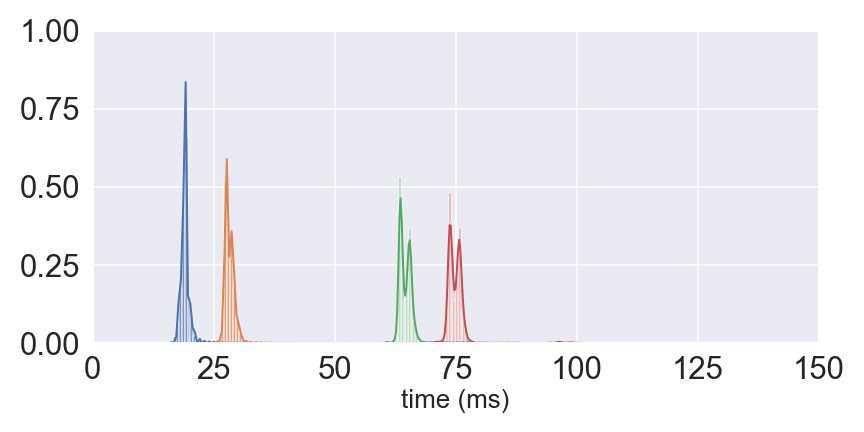
\includegraphics[width=\textwidth,height=.29\textheight,keepaspectratio]{figures/inference_plots/jetson_b-resnet_inference_time_distribution}}
		\hfill
		\subfloat[\gls{densenet} ]{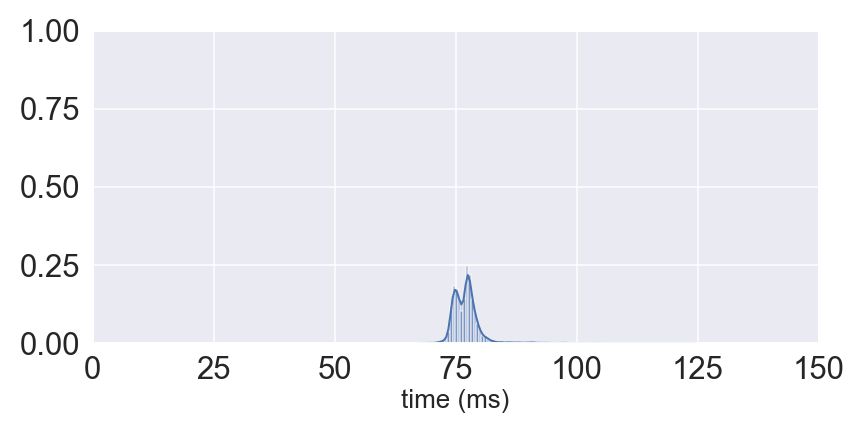
\includegraphics[width=\textwidth,height=.2\textheight,keepaspectratio]{figures/inference_plots/jetson_densenet_inference_time_distribution}}
		\hfill
		\subfloat[B-\gls{densenet}]{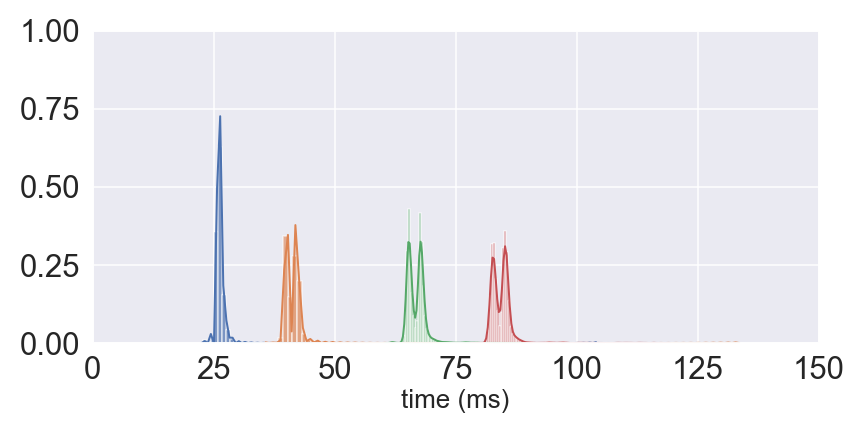
\includegraphics[width=\textwidth,height=.2\textheight,keepaspectratio]{figures/inference_plots/jetson_b-densenet_inference_time_distribution}}
		\hfill
		\subfloat[\gls{msdnet}]{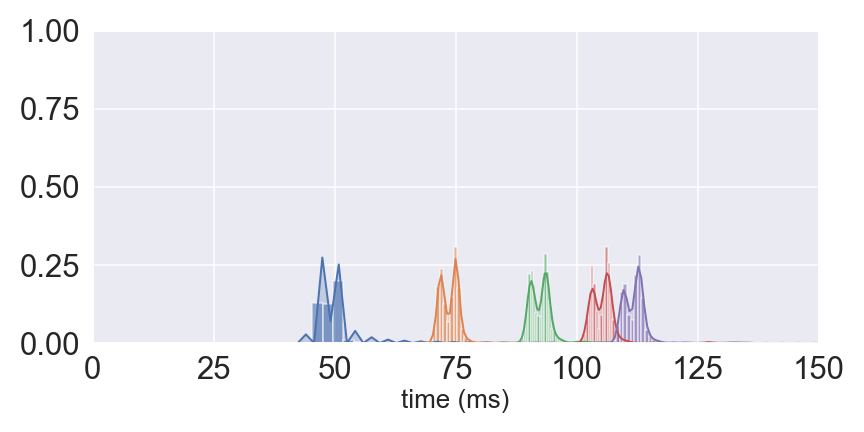
\includegraphics[width=\textwidth,height=.2\textheight,keepaspectratio]{figures/inference_plots/jetson_msdnet_inference_time_distribution}}
	\end{minipage}
	\begin{minipage}{.33\textwidth}
		\captionsetup[subfigure]{farskip=0pt,captionskip=0pt,justification=centering}
		\centering
		Intel NUC
		\subfloat[\gls{resnet} ]{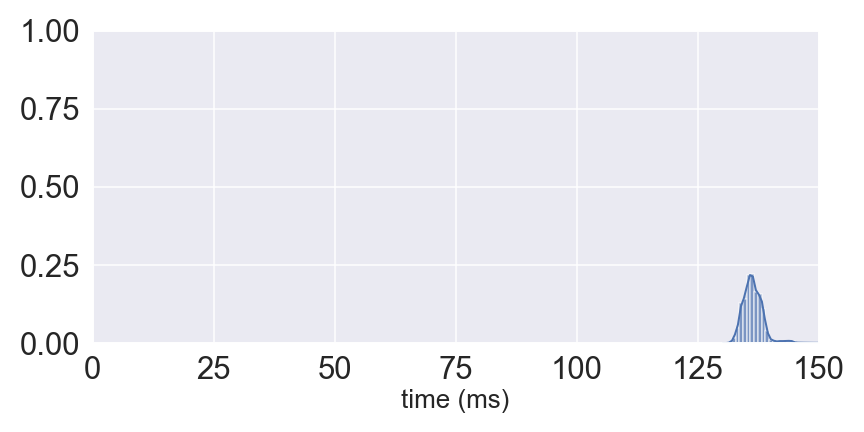
\includegraphics[width=\textwidth,keepaspectratio]{figures/inference_plots/nuc_resnet_inference_time_distribution}}
		\hfill
		\subfloat[B-\gls{resnet}]{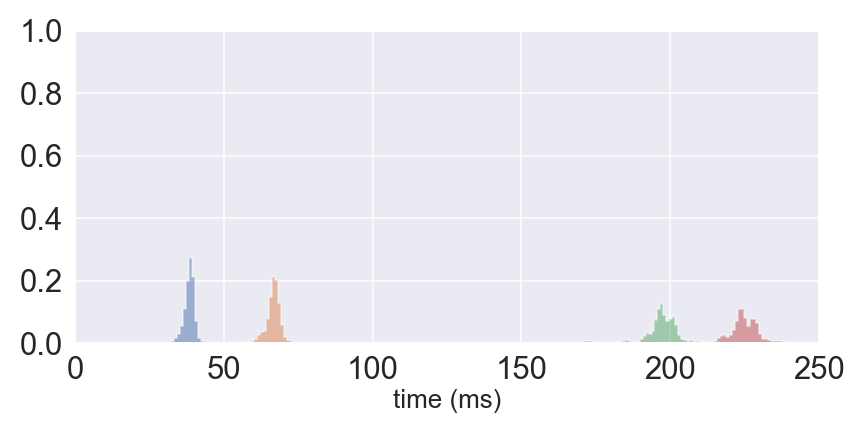
\includegraphics[width=\textwidth,height=.2\textheight,keepaspectratio]{figures/inference_plots/nuc_b-resnet_inference_time_distribution}}
		\hfill
		\subfloat[\gls{densenet} ]{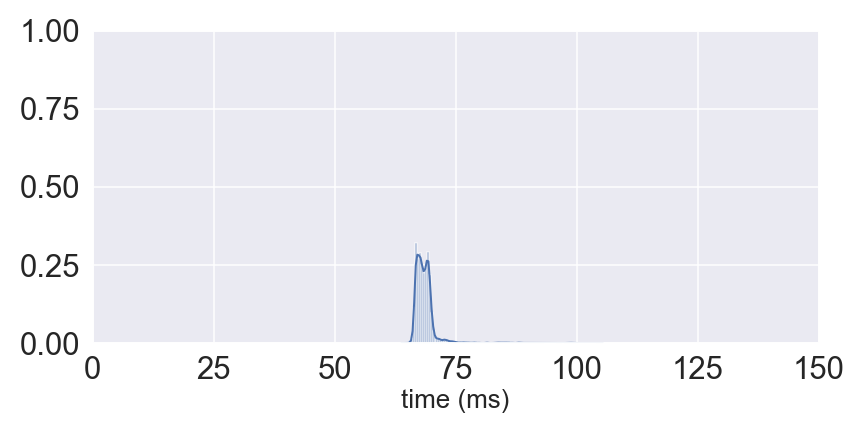
\includegraphics[width=\textwidth,keepaspectratio]{figures/inference_plots/nuc_densenet_inference_time_distribution}}
		\hfill
		\subfloat[B-\gls{densenet}]{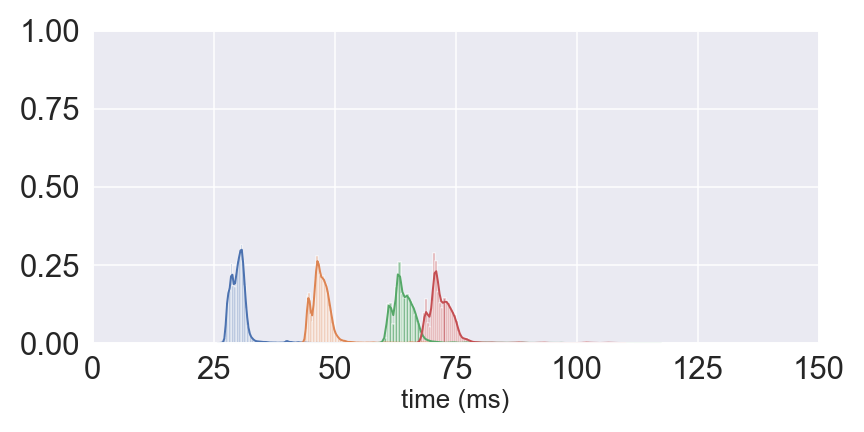
\includegraphics[width=\textwidth,keepaspectratio]{figures/inference_plots/nuc_b-densenet_inference_time_distribution}}
		\hfill
		\subfloat[\gls{msdnet}]{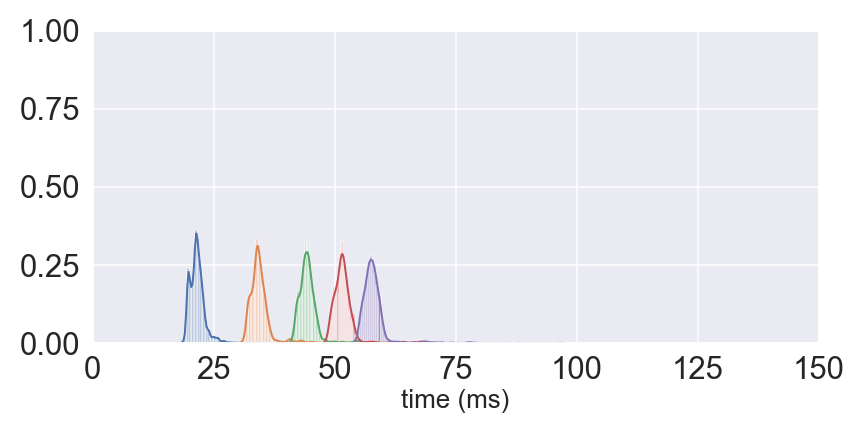
\includegraphics[width=\textwidth,keepaspectratio]{figures/inference_plots/nuc_msdnet_inference_time_distribution}}	
	\end{minipage}
	\caption[Platform Inference Time of \gls{dnn}s]{Inference Time Distribution, left column: GPU Workstation (a-e), center column: Jetson TX2 (f-j), right column NUC (k-o)}
	\label{fig:inference-time-dist}
\end{figure}

Research results in \cite{lee_energy_2019} state that \gls{densenet}'s and \gls{msdnet}’s linearly increasing amount of filters by continuous concatenation is inefficient on \gls{gpu}s due to expensive memory accessing on \gls{gpu}s. They propose a new design that still preserves information by concatenation. Instead, they only concatenate once at the end of a block, thereby achieving runtime superior to \gls{densenet}. They achieve comparable runtime and accuracy to \gls{resnet}. In \cite{lee_energy_2019}, they question if deep and thin networks are inefficient on \gls{gpu}s and argue that \gls{flop}s is not a good metric for \gls{gpu} efficiency. Instead, they propose \gls{flop}s/s. in \cite{zagoruyko_wide_2017}, they propose Wide-Residual Networks a more computational efficient version of \gls{resnet} by taking advantage of larger tensors that allow for more parallelization on \gls{gpu}s. The \gls{cpu}-only NUC cannot achieve the same level of parallelization to accelerate model inference. On the \gls{nuc}, the \gls{msdnet} outperforms the other models, as it requires far fewer \gls{flop}s and has far fewer layers and parameters. 
\subsubsection{Theoretical Exit Score Threshold Analysis}
We mentioned in section \ref{sec:ee-branchy-vs-cascaded} that a score threshold could be used to control the accuracy-latency trade-off of early exiting models. If a high threshold is selected, only a few samples can confidently exit the model at an early exit. Thus, no significant delay improvements may be found. On the contrary, if a low threshold is selected, a significant delay improvement may be found, but at a corresponding reduction of accuracy. 
In this experiment, we let all samples get classified at each exit until the end of the network. The purpose of this experiment is to conduct a theoretical study of the impact of the exit threshold. We log the predicted class label and score output. Using the two different score functions, $ f_{max} $ and $ f_{margin} $, we mark a sample \emph{exitable} if the output of the score function higher than the threshold. We analyse all models against a range of thresholds $ \gamma = \left\{0.1, 0.2, \dots 0,9\right\} $.
\Cref{fig:resnet_confidence,fig:resnet_score-margin,fig:densenet_confidence,fig:densenet_score-margin,fig:msdnet_confidence,fig:msdnet_score-margin} compare all exits at a rising threshold. We show the results for both score functions.
The figures show the frequency of exited samples that have been correctly exited ({\color{sns-green}green}), incorrectly exited samples ({\color{sns-red}red}), and the frequency of not exited samples ({\color{sns-blue}blue}). 

The growing frequency of correctly exited samples at later exits shows how the models become more accurate at deeper exits. The overall accuracy of the model is reduced if a sample exits incorrectly at an early exit, and it could have been correctly classified at a later exit. Raising the threshold reduces the amount of incorrectly exited samples but also reduces the frequency of correctly classified samples. 
By raising the score threshold, we aim to reduce the number of incorrectly exited samples more than we reduce the amount of correctly exited samples. The line shown on each subfigure ({\color{sns-orange}orange}) shows the change in exiting accuracy as we raise the score threshold. The exiting accuracy is the ratio of correctly classified samples out of all exited samples. Hence we do not account for not exited samples. 
Note, the exiting accuracy rises with the threshold; hence we reduce the amount of incorrectly exited samples. However, the amount of not exited samples also grows, which means inference is continued, and more latency can be expected.
The figures show that the score-margin has more desirable traits, as fewer samples are incorrectly exited. The result matches the study in \cite{park_big/little_2015,tann_flexible_2018}, showing a stronger correlation between score-margin and accuracy than between confidence score and accuracy. 

\newcounter{imagenumber}
\begin{center}
	\begin{minipage}{\textwidth}
		\begin{figure}
			\centering
			\paragraph{B-ResNet}
			\includegraphics[width=\linewidth]{figures/threshold_plots/threshold_analysis_legend}
		\end{figure}
		
		\begin{minipage}{0.5\textwidth}
			\begin{figure}
				\captionsetup[subfloat]{farskip=1pt,captionskip=1pt, justification=centering}
				\centering
				\forloop{imagenumber}{0}{\value{imagenumber} < 4}{
					
					\subfloat[Exit-\arabic{imagenumber}\label{fig:confidence_resnet_exit_\arabic{imagenumber}}]{\includegraphics[width=.9\linewidth]{figures/threshold_plots/threshold_analysis_b-resnet_confidence_\arabic{imagenumber}}}
					\hfill
				}
				\caption[ResNet Confidence Threshold]{Confidence Threshold}
				\label{fig:resnet_confidence}
			\end{figure}
		\end{minipage}
		\hfill
		\begin{minipage}{0.5\textwidth}
			\begin{figure}
				\captionsetup[subfloat]{farskip=1pt,captionskip=1pt, justification=centering}
				\centering
				\forloop{imagenumber}{0}{\value{imagenumber} < 4}{
					
					\subfloat[Exit-\arabic{imagenumber}\label{fig:score-margin_resnet_exit_\arabic{imagenumber}}]{\includegraphics[width=.9\linewidth]{figures/threshold_plots/threshold_analysis_b-resnet_score-margin_\arabic{imagenumber}}}
					\hfill
				}
				\caption[ResNet Score-margin Threshold]{Score-margin Threshold}
				\label{fig:resnet_score-margin}
			\end{figure}
		\end{minipage}
	\end{minipage}
\end{center}


\begin{center}
	\begin{minipage}{\textwidth}
		\begin{figure}
			\centering
			\paragraph{B-DenseNet}
		\end{figure}
		\begin{minipage}{0.5\textwidth}
			\begin{figure}
				\captionsetup[subfloat]{farskip=1pt,captionskip=1pt, justification=centering}
				\centering
				\forloop{imagenumber}{0}{\value{imagenumber} < 4}{
					
					\subfloat[Exit-\arabic{imagenumber}\label{fig:confidence_dense_exit_\arabic{imagenumber}}]{\includegraphics[width=.9\linewidth]{figures/threshold_plots/threshold_analysis_b-densenet_confidence_\arabic{imagenumber}}}
					\hfill
				}
				\caption[DenseNet Confidence Threshold]{Confidence Threshold}
				\label{fig:densenet_confidence}
			\end{figure}
		\end{minipage}
		\hfill
		\begin{minipage}{0.5\textwidth}
			\begin{figure}
				\captionsetup[subfloat]{farskip=1pt,captionskip=1pt, justification=centering}
				\centering
				\forloop{imagenumber}{0}{\value{imagenumber} < 4}{
					
					\subfloat[Exit-\arabic{imagenumber}\label{fig:score-dense_resnet_exit_\arabic{imagenumber}}]{\includegraphics[width=.9\linewidth]{figures/threshold_plots/threshold_analysis_b-densenet_score-margin_\arabic{imagenumber}}}
					\hfill
				}
				\caption[DenseNet Score-margin Threshold]{Score-margin Threshold}
				\label{fig:densenet_score-margin}
			\end{figure}
		\end{minipage}
	\end{minipage}
\end{center}


\noindent\makebox[\textwidth][c]{\begin{minipage}{0.9\textwidth}
		\begingroup
		\leftskip=0cm plus 0.5fil \rightskip=0cm plus -0.5fil
		\parfillskip=0cm plus 1fil
		\paragraph{MSDNet}\par
		\endgroup
		
		\begin{minipage}{0.5\textwidth}
			\begin{figure}
				\captionsetup[subfloat]{farskip=0pt,captionskip=0pt, justification=centering}
				\centering
				\forloop{imagenumber}{0}{\value{imagenumber} < 5}{
					
					\subfloat[Exit-\arabic{imagenumber}\label{fig:confidence_msd_exit_\arabic{imagenumber}}]{\includegraphics[width=.9\linewidth]{figures/threshold_plots/threshold_analysis_msdnet_confidence_\arabic{imagenumber}}}
					\hfill
				}
				\caption[MSDNet Confidence Threshold]{Confidence Threshold}
				\label{fig:msdnet_confidence}
			\end{figure}
		\end{minipage}
		\hfill
		\begin{minipage}{0.5\textwidth}
			\begin{figure}
				\captionsetup[subfloat]{farskip=1pt,captionskip=1pt, justification=centering}
				\centering
				\forloop{imagenumber}{0}{\value{imagenumber} < 5}{
					
					\subfloat[Exit-\arabic{imagenumber}\label{fig:score-msdnet_exit_\arabic{imagenumber}}]{\includegraphics[width=.9\linewidth]{figures/threshold_plots/threshold_analysis_msdnet_score-margin_\arabic{imagenumber}}}
					\hfill
				}
				\caption[MSDNet Score-margin Threshold]{Score-margin Threshold}
				\label{fig:msdnet_score-margin}
			\end{figure}
		\end{minipage}
\end{minipage}}

\subsubsection{Practical Exit Score Threshold Analysis}

In this section, we aim to evaluate the early existing capabilities of the different models in practice, where each exit has the same threshold. We experiment with raising the threshold for $ \gamma = \left\{0.1, 0.2, \dots 0,9\right\} $.  We exploit the exit mechanism to terminate inference if a satisfying score is obtained at an early exit. If a sample did not achieve a satisfying score on any of the early exits, it is classified by the last exit of the model. Figure \ref{fig:model_c-threshold_comparison} presents the result using the score-max and figure \ref{fig:model_threshold_comparison} using the score-margin. The subfigures show the raised score requirements. Each subfigure presents a subplot of the frequency of correctly exited samples and a subplot of incorrectly exit samples at each exit for all three models. 

\begin{minipage}{\linewidth}
	\begin{figure}
		\captionsetup[subfloat]{justification=centering, captionskip=0pt, farskip=0pt}
		\centering
		\includegraphics[width=.5\linewidth]{figures/inference_plots/model_bar_legend}
	\end{figure}
	\begin{figure}
		\captionsetup[subfloat]{justification=centering, captionskip=0pt, farskip=1pt}
		\centering
		\subfloat[$\gamma= 0.1$\label{fig:model-c-threshold_comparison_t_1}]{\includegraphics[width=.33\linewidth]{figures/inference_plots/model_confidence_comparison_1}}
		\hfill
		\subfloat[$\gamma= 0.2$\label{fig:model-c-threshold_comparison_t_2}]{\includegraphics[width=.33\linewidth]{figures/inference_plots/model_confidence_comparison_2}}
		\hfill
		\subfloat[$\gamma= 0.3$\label{fig:model-c-threshold_comparison_t_3}]{\includegraphics[width=.33\linewidth]{figures/inference_plots/model_confidence_comparison_3}}
		\hfill
		\subfloat[$\gamma= 0.4$\label{fig:model-c-threshold_comparison_t_4}]{\includegraphics[width=.33\linewidth]{figures/inference_plots/model_confidence_comparison_4}}
		\hfill
		\subfloat[$\gamma= 0.5$\label{fig:model-c-threshold_comparison_t_5}]{\includegraphics[width=.33\linewidth]{figures/inference_plots/model_confidence_comparison_5}}
		\hfill
		\subfloat[$\gamma= 0.6$\label{fig:model-c-threshold_comparison_t_6}]{\includegraphics[width=.33\linewidth]{figures/inference_plots/model_confidence_comparison_6}}
		\hfill
		\subfloat[$T= 0.7$\label{fig:model-c-threshold_comparison_t_7}]{\includegraphics[width=.33\linewidth]{figures/inference_plots/model_confidence_comparison_7}}
		\hfill
		\subfloat[$\gamma= 0.8$\label{fig:model-c-threshold_comparison_t_8}]{\includegraphics[width=.33\linewidth]{figures/inference_plots/model_confidence_comparison_8}}
		\hfill
		\subfloat[$\gamma= 0.9$\label{fig:model-c-threshold_comparison_t_9}]{\includegraphics[width=.33\linewidth]{figures/inference_plots/model_confidence_comparison_9}}
		
		\caption[Model comparison of early exit capabilities using confidence threshold]{Model comparison of early exit capabilities using score-max}
		\label{fig:model_c-threshold_comparison}
	\end{figure}
	
\end{minipage}

\begin{minipage}{\linewidth}
	\begin{figure}
		\captionsetup[subfloat]{justification=centering, captionskip=0pt, farskip=0pt}
		\centering
		\includegraphics[width=.5\linewidth]{figures/inference_plots/model_bar_legend}
	\end{figure}
	\begin{figure}
		\captionsetup[subfloat]{justification=centering, captionskip=0pt, farskip=1pt}
		\centering
		\subfloat[$\gamma= 0.1$\label{fig:model-threshold_comparison_t_1}]{\includegraphics[width=.33\linewidth]{figures/inference_plots/model_comparison_1}}
		\hfill
		\subfloat[$\gamma= 0.2$\label{fig:model-threshold_comparison_t_2}]{\includegraphics[width=.33\linewidth]{figures/inference_plots/model_comparison_2}}
		\hfill
		\subfloat[$\gamma= 0.3$\label{fig:model-threshold_comparison_t_3}]{\includegraphics[width=.33\linewidth]{figures/inference_plots/model_comparison_3}}
		\hfill
		\subfloat[$\gamma= 0.4$\label{fig:model-threshold_comparison_t_4}]{\includegraphics[width=.33\linewidth]{figures/inference_plots/model_comparison_4}}
		\hfill
		\subfloat[$T= 0.5$\label{fig:model-threshold_comparison_t_5}]{\includegraphics[width=.33\linewidth]{figures/inference_plots/model_comparison_5}}
		\hfill
		\subfloat[$\gamma= 0.6$\label{fig:model-threshold_comparison_t_6}]{\includegraphics[width=.33\linewidth]{figures/inference_plots/model_comparison_6}}
		\hfill
		\subfloat[$\gamma= 0.7$\label{fig:model-threshold_comparison_t_7}]{\includegraphics[width=.33\linewidth]{figures/inference_plots/model_comparison_7}}
		\hfill
		\subfloat[$\gamma= 0.8$\label{fig:model-threshold_comparison_t_8}]{\includegraphics[width=.33\linewidth]{figures/inference_plots/model_comparison_8}}
		\hfill
		\subfloat[$\gamma= 0.9$\label{fig:model-threshold_comparison_t_9}]{\includegraphics[width=.33\linewidth]{figures/inference_plots/model_comparison_9}}
		
		\caption[Model comparison of early exit capabilities]{Model comparison of early exit capabilities using score-margin}
		\label{fig:model_threshold_comparison}
	\end{figure}
	
\end{minipage}

Notice, only a few numbers of samples require the last exits for any of the models. Especially at low thresholds, the last exit is unused. As the threshold is raised, we force the model more frequently use later exits. The result is that fewer samples are incorrectly classified at early exits. \gls{bdensenet} and especially \gls{msdnet}, can more frequently exit samples at the earliest exits even at high thresholds values, whereas \gls{bresnet} requires significantly more samples to exit at its second last exit.
Note, for each threshold setting, the frequency of correctly and incorrectly classification for each model sum to one, i.e., summing all blue bars for the \gls{resnet}, is equivalent to all samples of the test.

This result indicates that we can reduce the average inference delay by using the exit condition. In the next section, we evaluate the score threshold's impact on the accuracy-latency trade-off.
\subsubsection{Score Threshold and the Accuracy-Latency Trade-Off}
We inference all validation samples. We measure the time for a prediction to exit for raised score threshold $ \gamma = \left\{0.1, 0.2, \dots 0,9\right\} $. We let samples exit the inference using the score-margin function and log the prediction result. Figure \ref{fig:threshold-acc-lat-trade-off} shows the inference accuracy and latency of all the models on the platforms. The figure indicates the accuracy-latency trade-off implied by the early exit model.
\begin{figure}
	\captionsetup[subfigure]{justification=centering,farskip=0pt,captionskip=0pt}
	\centering
	\includegraphics[width=.4\linewidth]{figures/threshold_plots/inference_legend}
	\subfloat[GPU Workstation\label{fig:early_exit_vs_conv}]{\includegraphics[width=\textwidth,height=.22\textheight,keepaspectratio]{figures/threshold_plots/gpu_inference}}
	\hfill
	\subfloat[Jetson TX2\label{fig:jetson-early_exit_vs_conv}]{\includegraphics[width=\textwidth,height=.22\textheight,keepaspectratio]{figures/threshold_plots/jetson_inference}}
	\hfill
	\subfloat[NUC\label{fig:nuc-early_exit_vs_conv}]{\includegraphics[width=\textwidth,height=.22\textheight,keepaspectratio]{figures/threshold_plots/nuc_inference}}
	\caption[Threshold Accuracy-Latency Trade-off]{Threshold Accuracy-Latency Trade-off on \protect\subref{fig:early_exit_vs_conv} GPU Workstation, \protect\subref{fig:jetson-early_exit_vs_conv} Jetson TX2 and \protect\subref{fig:nuc-early_exit_vs_conv} NUC }
	\label{fig:threshold-acc-lat-trade-off}
\end{figure}

Raising the score threshold improves the models' accuracy but also introduces more latency. We showed in the previous section that raising the score threshold forces the model to use deeper exits more frequently. The raises threshold result in additional delay. In figure \ref{fig:threshold-acc-lat-trade-off-by-time} and \ref{fig:threshold-acc-lat-trade-off}, we show the accuracy-latency tradeoff by plotting accuracy against the meantime.
\begin{figure}
	\captionsetup[subfigure]{justification=centering,farskip=0pt,captionskip=0pt}
	\centering
	\includegraphics[width=.4\linewidth]{figures/threshold_plots/inference_by_time_legend}
	\subfloat[GPU Workstation\label{fig:gpu-early_exit_vs_time}]{\includegraphics[width=\textwidth,height=.22\textheight,keepaspectratio]{figures/threshold_plots/gpu_inference_by_time}}
	\hfill
	\subfloat[Jetson TX2\label{fig:jetson-early_exit_vs_time}]{\includegraphics[width=\textwidth,height=.22\textheight,keepaspectratio]{figures/threshold_plots/jetson_inference_by_time}}
	\hfill
	\subfloat[NUC\label{fig:nuc-early_exit_vs_time}]{\includegraphics[width=\textwidth,height=.22\textheight,keepaspectratio]{figures/threshold_plots/nuc_inference_by_time}}
	\caption[Threshold Accuracy-Latency Trade-off]{Threshold Accuracy-Latency Trade-off on \protect\subref{fig:early_exit_vs_conv} GPU Workstation, \protect\subref{fig:jetson-early_exit_vs_conv} Jetson TX2 and \protect\subref{fig:nuc-early_exit_vs_conv} NUC }
	\label{fig:threshold-acc-lat-trade-off-by-time}
\end{figure}

The flexibility of the early exit models shows that when more time is available, higher accuracy can be achieved. The conventional models are inflexible as no early exit is present. Even though they can achieve higher accuracy, they also require more time.
For the accuracy-latency trade-off on the \gls{gpu}-workstation and the Jetson, the \gls{bresnet} is outperforming the other models. On the NUC, \gls{bresnet} is the worst performing, and the \gls{msdnet} is outperforming the others. In table \ref{tbl:score-acc-lat-trade}, the change in accuracy and time using different thresholds compared to let the inference run to the end.
A low threshold gives a significant reduction in inference latency, however, also at the cost of accuracy. Significant time saving is still possible when selecting a high threshold, which only introduces a small cost of accuracy. Some overthinking is mitigated when selecting a high threshold, as minor improvement of accuracy is found using a threshold value of 0.9 for both \gls{resnet} and \gls{densenet}.
\begin{minipage}[t]{\linewidth}\begin{small}
		
		\begin{longtabu}{>{\bfseries}X|X|X[r]|X[r]|X[r]|X[r]}
			\caption[Score Threshold Accuracy-Latency Trade-off]{Score Threshold Accuracy-Latency Trade-off. The table shows the impact of score threshold on accuracy and latency. The table compares running the early exit model all the wat to the end with letting samples exit based on the score.}\label{tbl:score-acc-lat-trade} \\
			\toprule
			\rowfont{\bfseries}
			& & & {GPU Workstation} &  {Jetson TX2} & {Intel NUC} \tabularnewline
			\rowfont{\bfseries} Model & Threshold & Acc. dif. & Time dif. (ms)  & Time dif. (ms) & Time dif. (ms) \tabularnewline
			\hline
			\endfirsthead
			\multicolumn{3}{@{}l}{\textbf{\textcolor{black}{Table \ref{tbl:score-acc-lat-trade}:}} continued}\\
			\toprule
			\rowfont{\bfseries}
			& &  & {GPU Workstation} &  {Jetson TX2} & {Intel NUC} \tabularnewline
			\rowfont{\bfseries} Model & Threshold & Acc. dif. & Time dif. (ms)  & Time dif. (ms) & Time dif. (ms) \tabularnewline
			\hline
			\endhead % all the lines above this will be repeated on every page
			\hline
			\multicolumn{3}{@{}l}{continued \ldots}\\
			\endfoot
			\hline
			\multirow{11}{*}{B-ResNet} & End (No Exit) & 0.88 & 37.14 & 67.04 & 223.32  \tabularnewline \tabucline{2-7}
			& $ \gamma = 0.1 $ 	& -0.24 & -19.76 & -40.87 & -181.53 \tabularnewline
			&$ \gamma = 0.2 $ 	& -0.15 & -16.10 & -36.11 & -171.44 \tabularnewline 
			&$ \gamma = 0.3 $ 	& -0.09 & -13.45 & -32.16 & -163.55 \tabularnewline
			&$ \gamma = 0.4 $ 	& -0.06 & -10.91 & -28.63 & -155.14 \tabularnewline 
			&$ \gamma = 0.5 $ 	& -0.03 &  -8.93 & -25.72 & -150.43 \tabularnewline
			&$ \gamma = 0.6 $ 	& -0.02 &  -7.20 & -23.01 & -144.25 \tabularnewline 
			&$ \gamma = 0.7 $ 	& -0.01 &  -5.09 & -20.16 & -141.93 \tabularnewline 
			&$ \gamma = 0.8 $ 	&  0.00 &  -3.39 & -17.34 & -136.39 \tabularnewline 
			&$ \gamma = 0.9 $ 	&  0.01 &  -0.40 & -13.24 & -127.15 \tabularnewline 
			\hline
			\multirow{11}{*}{B-DenseNet} & End (No Exit) & 0.87 & 49.14 & 72.40 & 72.21 \tabularnewline \tabucline{2-7}
			&$ \gamma = 0.1 $ 	& -0.21 & -27.08 & -40.33 & -36.65  \tabularnewline
			&$ \gamma = 0.2 $ 	& -0.14 & -24.04 & -37.60 & -33.54  \tabularnewline 
			&$ \gamma = 0.3 $ 	& -0.10 & -21.37 & -34.29 & -31.35  \tabularnewline
			&$ \gamma = 0.4 $ 	& -0.07 & -19.02 & -31.41 & -27.30  \tabularnewline 
			&$ \gamma = 0.5 $ 	& -0.04 & -16.94 & -28.77 & -25.00  \tabularnewline
			&$ \gamma = 0.6 $ 	& -0.03 & -14.57 & -26.07 & -25.17  \tabularnewline 
			&$ \gamma = 0.7 $ 	& -0.01 & -12.70 & -23.90 & -22.67  \tabularnewline 
			&$ \gamma = 0.8 $ 	&  0.00 & -10.32 & -20.95 & -18.66  \tabularnewline 
			&$ \gamma = 0.9 $ 	&  0.01 &  -6.94 & -17.07 & -17.85  \tabularnewline 
			\hline
			\multirow{11}{*}{MSDNet} & End (No Exit) & 0.86 & 68.87 & 103.29 & 56.02 \tabularnewline \tabucline{2-7}
			&$ \gamma = 0.1 $ 	& -0.09 & -29.52 & -51.30 & -33.14 \tabularnewline
			&$ \gamma = 0.2 $ 	& -0.08 & -28.15 & -50.39 & -32.45 \tabularnewline 
			&$ \gamma = 0.3 $ 	& -0.06 & -26.83 & -48.53 & -31.61 \tabularnewline
			&$ \gamma = 0.4 $ 	& -0.05 & -25.31 & -47.06 & -30.93 \tabularnewline 
			&$ \gamma = 0.5 $ 	& -0.04 & -23.95 & -45.31 & -29.81 \tabularnewline
			&$ \gamma = 0.6 $ 	& -0.03 & -22.32 & -43.40 & -28.86 \tabularnewline 
			&$ \gamma = 0.7 $ 	& -0.02 & -20.28 & -41.39 & -27.38 \tabularnewline 
			&$ \gamma = 0.8 $ 	& -0.01 & -17.79 & -38.73 & -25.88 \tabularnewline 
			&$ \gamma = 0.9 $ 	& -0.00 & -14.32 & -34.46 & -23.44 \tabularnewline 
			\bottomrule
		\end{longtabu}
	\end{small}
\end{minipage}

We have shown that the early exit model can be used to reduce the latency with a compromise in accuracy when controlled by a score threshold. However, can we use early exits \gls{dnn} to meet the delay requirement for time-critical application? 

\newpage\subsubsection{Reliability vs. Computation Latency}

We let all the validation samples inference the early exit models and let all exits classify all samples.  We aim to maximize reliability. We use 0.1 ms granularity by setting the delay threshold $\delta = \{0,0.1,0.1, \dots, 250,0\}$. In figure \ref{fig:delay-threshold}, we show the achieved reliability for the delay threshold. 
\begin{figure}
	\captionsetup[subfigure]{justification=centering, farskip=0pt,captionskip=0pt}
	\centering
	\includegraphics[height=.05\textheight]{figures/delay_plots/delay_threshold_legend}
	\hfill
	\subfloat[GPU Workstation]{\includegraphics[width=\textwidth,height=.22\textheight,keepaspectratio]{figures/delay_plots/gpu__delay_threshold}}
	\hfill
	\subfloat[Jetson TX2]{\includegraphics[width=\textwidth,height=.22\textheight,keepaspectratio]{figures/delay_plots/jetson__delay_threshold}}
	\hfill
	\subfloat[NUC]{\includegraphics[width=\textwidth,height=.22\textheight,keepaspectratio]{figures/delay_plots/nuc__delay_threshold}}
	\caption[Reliability vs. Computation Latency]{Reliability vs. Delay Threshold}
	\label{fig:delay-threshold}
\end{figure}
The figure shows a staircase-like graph of reliability. As we relax the delay constraint, higher reliability can be obtained, since more time is available. The steps of the graph show when a later exit becomes available within the delay constraint. The dashed lines show the inference time for the conventional models. Using early exit models, we can improve the reliability of the more stringent delay threshold. We enable \gls{ai}-driven service not even possible for the conventional model. The conventional model is inflexible and has only one step when service becomes possible. Thus, the conventional model is more prone to unexpected delays. However, if the last exit of the early exit model is reachable, then the conventional models will achieve superior reliability due to the model being more accurate under relaxed constraints. 

\section{Summary} \label{sec:ee-summary}
We have successfully trained three early exiting models on the \gls{min100} dataset. We have shown that freezing the model base, as proposed in \cite{leroux_resource-constrained_2015}, did not allow features to be optimized classifiers at early exits. Training the entire early exit model, as in \cite{teerapittayanon_branchynet:_2016}, significantly improved the validation accuracy. The \gls{msdnet} obtains the highest accuracy for early exits, but \gls{bresnet} obtains higher accuracy at the last two exits. 
We measured inference time on three hardware platforms. The inference times are hardware dependent. The \gls{gpu-ws} are enabled with the most powerful \gls{gpu} and has most parallelization capabilities, which makes it able to run, especially \gls{resnet}, significantly faster \cite{lee_energy_2019}. However, \gls{densenet} and \gls{msdnet} have significantly fewer parameters and require fewer \gls{flop}s, hence when less parallelization is possible, these models achieve faster runtimes.
We investigated score thresholds as a mechanism to exit samples early. We used both score-max and score-margin. The max score confidence threshold is widely used in early exiting literature \cite{leroux_resource-constrained_2015, leroux_cascading_2017, kaya_shallow-deep_nodate, berestizshevsky_sacrificing_2019}. The score-margin has not been used directly for early exiting but used in model selection frameworks \cite{park_big/little_2015,tann_flexible_2018}. The score-margin was able to remove most incorrectly exited samples when choosing a sufficiently high threshold value. Additionally, we compared the early exit capabilities of the models. The model comprised of densely connected blocks \gls{bdensenet} and \gls{msdnet} were able to correctly exit more samples at early exits, where the model designed for early exiting, \gls{msdnet} outperformed its competitors. 
We studied the accuracy-latency trade-off for early exit models. Early exit models can reduce runtime compared to conventional models. The \gls{bresnet} has shown to be the best model at making a compromise between accuracy and latency on the \gls{gpu}-enabled platforms. In sharp contrast to the accuracy-latency trade-off on the NUC. On the NUC both the \gls{bdensenet} and \gls{msdnet} were better than \gls{bresnet}.
Finally, we evaluated the reliability under different delay threshold. The conventional models are outperformed at stringent delay thresholds. \gls{bresnet} is still the better model on the \gls{gpu}-enabled platforms. However, not as exclusively as figure \ref{fig:threshold-acc-lat-trade-off-by-time} shows when using a score threshold. Figure \ref{fig:delay-threshold} shows that for certain delay thresholds, \gls{bdensenet} is better. For the \gls{nuc}, the \gls{msdnet} was the best choice.
Figure \ref{fig:delay-threshold} encourages model selection, where the most reliable model is chosen based on the required delay threshold.
